% -*- Mode:TeX -*-

%% IMPORTANT: The official thesis specifications are available at:
%%            http://libraries.mit.edu/archives/thesis-specs/
%%
%%            Please verify your thesis' formatting and copyright
%%            assignment before submission.  If you notice any
%%            discrepancies between these templates and the 
%%            MIT Libraries' specs, please let us know
%%            by e-mailing thesis@mit.edu

%% The documentclass options along with the pagestyle can be used to generate
%% a technical report, a draft copy, or a regular thesis.  You may need to
%% re-specify the pagestyle after you \include  cover.tex.  For more
%% information, see the first few lines of mitthesis.cls. 

%\documentclass[12pt,vi,twoside]{mitthesis}
%%
%%  If you want your thesis copyright to you instead of MIT, use the
%%  ``vi'' option, as above.
%%
%\documentclass[12pt,twoside,leftblank]{mitthesis}
%%
%% If you want blank pages before new chapters to be labelled ``This
%% Page Intentionally Left Blank'', use the ``leftblank'' option, as
%% above. 

\documentclass[12pt,twoside]{mitthesis}
\usepackage{lgrind}
\usepackage{url}
\usepackage{acronym}
\usepackage[colorlinks=true,urlcolor=black,colorlinks=true,linkcolor=black,citecolor=black,filecolor=black,urlcolor=black,]{hyperref}
\usepackage{tabularx}
\usepackage{multirow}
\usepackage{fancyref}
\usepackage{caption}
\usepackage{subcaption}
\usepackage{graphicx} 
\usepackage[gen]{eurosym}
\usepackage{listings, color}
%\usepackage[backend=bibtex,url=true]{biblatex} 
\usepackage{misc/packages/risk-tpl}
\usepackage{xkeyval}
\usepackage{rotating}
\usepackage{placeins}
\usepackage{xspace}

\pagestyle{plain}

\definecolor{gray}{rgb}{0.4,0.4,0.4}
\definecolor{darkblue}{rgb}{0.0,0.0,0.6}
\definecolor{cyan}{rgb}{0.0,0.6,0.6}
\definecolor{lightgray}{rgb}{.9,.9,.9}
\definecolor{darkgray}{rgb}{.4,.4,.4}
\definecolor{purple}{rgb}{0.65, 0.12, 0.82}
 
\lstset{
  basicstyle=\ttfamily,
  numbers=left,
  lineskip={-1.5pt} ,
  columns=fullflexible,
  showstringspaces=false,
  commentstyle=\color{gray}\upshape
}
 
\lstdefinelanguage{XML}
{
  basicstyle=\ttfamily\color{darkblue}\bfseries,
  morestring=[b]",
  morestring=[s]{>}{<},
  morecomment=[s]{<?}{?>},
  stringstyle=\color{black},
  identifierstyle=\color{darkblue},
  keywordstyle=\color{cyan},
  morekeywords={xmlns,version,type, id, lang, src, caption, x, y, width, height, loop, loopy, loopx, scrolly, scrollx, scroll}% list your attributes here
}

\lstdefinelanguage{JavaScript}{
  keywords={typeof, new, true, false, catch, function, return, null, catch, switch, var, if, in, while, do, else, case, break},
  keywordstyle=\color{blue}\bfseries,
  ndkeywords={class, export, boolean, throw, implements, import, this},
  ndkeywordstyle=\color{darkgray}\bfseries,
  identifierstyle=\color{black},
  sensitive=false,
  comment=[l]{//},
  morecomment=[s]{/*}{*/},
  commentstyle=\color{purple}\ttfamily,
  stringstyle=\color{red}\ttfamily,
  morestring=[b]',
  morestring=[b]"
}

%% This bit allows you to either specify only the files which you wish to
%% process, or `all' to process all files which you \include.
%% Krishna Sethuraman (1990).

%\typein [\files]{Enter file names to process, (chap1,chap2 ...), or `all' to process all files:}
%\def\all{all}
%\ifx\files\all \typeout{Including all files.} \else \typeout{Including only \files.} %\includeonly{\files} \fi

\begin{document}

% -*-latex-*-
% 
% For questions, comments, concerns or complaints:
% thesis@mit.edu
% 
%
% $Log: cover.tex,v $
% Revision 1.8  2008/05/13 15:02:15  jdreed
% Degree month is June, not May.  Added note about prevdegrees.
% Arthur Smith's title updated
%
% Revision 1.7  2001/02/08 18:53:16  boojum
% changed some \newpages to \cleardoublepages
%
% Revision 1.6  1999/10/21 14:49:31  boojum
% changed comment referring to documentstyle
%
% Revision 1.5  1999/10/21 14:39:04  boojum
% *** empty log message ***
%
% Revision 1.4  1997/04/18  17:54:10  othomas
% added page numbers on abstract and cover, and made 1 abstract
% page the default rather than 2.  (anne hunter tells me this
% is the new institute standard.)
%
% Revision 1.4  1997/04/18  17:54:10  othomas
% added page numbers on abstract and cover, and made 1 abstract
% page the default rather than 2.  (anne hunter tells me this
% is the new institute standard.)
%
% Revision 1.3  93/05/17  17:06:29  starflt
% Added acknowledgements section (suggested by tompalka)
% 
% Revision 1.2  92/04/22  13:13:13  epeisach
% Fixes for 1991 course 6 requirements
% Phrase "and to grant others the right to do so" has been added to 
% permission clause
% Second copy of abstract is not counted as separate pages so numbering works
% out
% 
% Revision 1.1  92/04/22  13:08:20  epeisach

% NOTE:
% These templates make an effort to conform to the MIT Thesis specifications,
% however the specifications can change.  We recommend that you verify the
% layout of your title page with your thesis advisor and/or the MIT 
% Libraries before printing your final copy.
\title{Reengineering a Content Manager for Humanoid Robots with Web Technology}

\author{Eduard Gamonal Capdevila}
% If you wish to list your previous degrees on the cover page, use the 
% previous degrees command:
%       \prevdegrees{A.A., Harvard University (1985)}
% You can use the \\ command to list multiple previous degrees
%       \prevdegrees{B.S., University of California (1978) \\
%                    S.M., Massachusetts Institute of Technology (1981)}
\department{\Fib}

% If the thesis is for two degrees simultaneously, list them both
% separated by \and like this:
% \degree{Doctor of Philosophy \and Master of Science}
\degree{Master in Information Technology}

% As of the 2007-08 academic year, valid degree months are September, 
% February, or June.  The default is June.
\degreemonth{December}
\degreeyear{2013}
\thesisdate{Dec 18, 2013}

%% By default, the thesis will be copyrighted to MIT.  If you need to copyright
%% the thesis to yourself, just specify the `vi' documentclass option.  If for
%% some reason you want to exactly specify the copyright notice text, you can
%% use the \copyrightnoticetext command.  

\copyrightnoticetext{\copyright This work is licensed under the Creative Commons Attribution 4.0 International License. To view a copy of this license, visit \url{http://creativecommons.org/licenses/by/4.0/}.}

% If there is more than one supervisor, use the \supervisor command
% once for each.
%\supervisor{N\'{u}ria Castell Ari\~{n}o}

% This is the department committee chairman, not the thesis committee
% chairman.  You should replace this with your Department's Committee
% Chairman.
%\chairman{Daniel Pinyol}{CTO at \company}

% Make the titlepage based on the above information.  If you need
% something special and can't use the standard form, you can specify
% the exact text of the titlepage yourself.  Put it in a titlepage
% environment and leave blank lines where you want vertical space.
% The spaces will be adjusted to fill the entire page.  The dotted
% lines for the signatures are made with the \signature command.
\maketitle

% The abstractpage environment sets up everything on the page except
% the text itself.  The title and other header material are put at the
% top of the page, and the supervisors are listed at the bottom.  A
% new page is begun both before and after.  Of course, an abstract may
% be more than one page itself.  If you need more control over the
% format of the page, you can use the abstract environment, which puts
% the word "Abstract" at the beginning and single spaces its text.

%% You can either \input (*not* \include) your abstract file, or you can put
%% the text of the abstract directly between the \begin{abstractpage} and
%% \end{abstractpage} commands.

% First copy: start a new page, and save the page number.

\cleardoublepage
% Uncomment the next line if you do NOT want a page number on your
% abstract and acknowledgments pages.
\pagestyle{empty}
\setcounter{savepage}{\thepage}

\begin{abstractpage}

% $Log: abstract.tex,v $
% Revision 1.1  93/05/14  14:56:25  starflt
% Initial revision
% 
% Revision 1.1  90/05/04  10:41:01  lwvanels
% Initial revision
% 
%
%% The text of your abstract and nothing else (other than comments) goes here.
%% It will be single-spaced and the rest of the text that is supposed to go on
%% the abstract page will be generated by the abstractpage environment.  This
%% file should be \input (not \include 'd) from cover.tex.

This project aims at reengineering a content manager for humanoid robots with web technology at \company in order to abandon the current \flash implementation.
This software in the robot displays content applications and handles user interaction.

In the first part, this thesis describes the boundaries and context of the project and provides a general overview of related topics that support this work.

In the second part, this thesis addresses the reengineering of the software based on Pressman's work, in 6 steps: software inventory, documentation restructure and reverse engineering, code and data restructuring and forward engineering.

First it identifies the constraints of the project as well as its functional and non-functional requirements.

Secondly, it presents the specification emphasising the first 3 steps.
This work includes a conceptual model, system use cases and sequence diagrams.

Thirdly, it describes the internal design of the system in the context of the last 3 steps.
It starts by highlighting the system's architecture, its context and the software patterns.
Fourthly, it provides a static view with class and packages diagram, a dynamic view with sequence diagrams and a physical view with a deployment diagram.

The following chapter provides an overview of the most relevant parts of the implementation with code examples.

Finally, it outlines the testing strategy and explains the testing system's implementation.

In conclusion, this master's thesis addresses the development of the new system with accuracy and consistency and describes the construction of the software applying a systematic approach, proven techniques like software patterns and architectures, and creativity.



\end{abstractpage}

% Additional copy: start a new page, and reset the page number.  This way,
% the second copy of the abstract is not counted as separate pages.
% Uncomment the next 6 lines if you need two copies of the abstract
% page.
% \setcounter{page}{\thesavepage}
% \begin{abstractpage}
% % $Log: abstract.tex,v $
% Revision 1.1  93/05/14  14:56:25  starflt
% Initial revision
% 
% Revision 1.1  90/05/04  10:41:01  lwvanels
% Initial revision
% 
%
%% The text of your abstract and nothing else (other than comments) goes here.
%% It will be single-spaced and the rest of the text that is supposed to go on
%% the abstract page will be generated by the abstractpage environment.  This
%% file should be \input (not \include 'd) from cover.tex.

This project aims at reengineering a content manager for humanoid robots with web technology at \company in order to abandon the current \flash implementation.
This software in the robot displays content applications and handles user interaction.

In the first part, this thesis describes the boundaries and context of the project and provides a general overview of related topics that support this work.

In the second part, this thesis addresses the reengineering of the software based on Pressman's work, in 6 steps: software inventory, documentation restructure and reverse engineering, code and data restructuring and forward engineering.

First it identifies the constraints of the project as well as its functional and non-functional requirements.

Secondly, it presents the specification emphasising the first 3 steps.
This work includes a conceptual model, system use cases and sequence diagrams.

Thirdly, it describes the internal design of the system in the context of the last 3 steps.
It starts by highlighting the system's architecture, its context and the software patterns.
Fourthly, it provides a static view with class and packages diagram, a dynamic view with sequence diagrams and a physical view with a deployment diagram.

The following chapter provides an overview of the most relevant parts of the implementation with code examples.

Finally, it outlines the testing strategy and explains the testing system's implementation.

In conclusion, this master's thesis addresses the development of the new system with accuracy and consistency and describes the construction of the software applying a systematic approach, proven techniques like software patterns and architectures, and creativity.


% \end{abstractpage}

\cleardoublepage

\begin{quotation}
\em
\medskip
\raggedleft
Any sufficiently advanced technology is indistinguishable from magic
\end{quotation}
\section*{Acknowledgments}

This is the acknowledgements section.  You should replace this with your
own acknowledgements.

%%%%%%%%%%%%%%%%%%%%%%%%%%%%%%%%%%%%%%%%%%%%%%%%%%%%%%%%%%%%%%%%%%%%%%
% -*-latex-*-

% Some departments (e.g. 5) require an additional signature page.  See
% signature.tex for more information and uncomment the following line if
% applicable.
% % -*- Mode:TeX -*-
%
% Some departments (e.g. Chemistry) require an additional cover page
% with signatures of the thesis committee.  Please check with your
% thesis advisor or other appropriate person to determine if such a 
% page is required for your thesis.  
%
% If you choose not to use the "titlepage" environment, a \newpage
% commands, and several \vspace{\fill} commands may be necessary to
% achieve the required spacing.  The \signature command is defined in
% the "mitthesis" class
%
% The following sample appears courtesy of Ben Kaduk <kaduk@mit.edu> and
% was used in his June 2012 doctoral thesis in Chemistry. 

\begin{titlepage}
\begin{large}
This doctoral thesis has been examined by a Committee of the Department
of Chemistry as follows:

\signature{Professor Jianshu Cao}{Chairman, Thesis Committee \\
   Professor of Chemistry}

\signature{Professor Troy Van Voorhis}{Thesis Supervisor \\
   Associate Professor of Chemistry}

\signature{Professor Robert W. Field}{Member, Thesis Committee \\
   Haslam and Dewey Professor of Chemistry}
\end{large}
\end{titlepage}


\pagestyle{plain}
  % -*- Mode:TeX -*-
%% This file simply contains the commands that actually generate the table of
%% contents and lists of figures and tables.  You can omit any or all of
%% these files by simply taking out the appropriate command.  For more
%% information on these files, see appendix C.3.3 of the LaTeX manual. 
\tableofcontents
\newpage
\listoffigures
\newpage
\listoftables
\newpage
\lstlistoflistings


% FIXME should acronyms go here?
\newpage
\begin{singlespace}

\begin{acronym}[TDMA]
   \acro{UPC}{Universitat Politecnica de Catalunya (Technical University of Catalonia)}
   \acro{RIA}{Rich Internet Application}
   \acro{XML}{Extensible Mark-up Language}
   \acro{HTML}{Hyper Text Mark-up Language}
   \acro{HTML5}{Hyper Text Mark-up Language 5}
   \acro{UI}{User Interface}
   \acro{WWW}{World Wide Web}
   \acro{CSS}{Cascading Style Sheet}
   \acro{CSS3}{Cascading Style Sheet 3}
   \acro{MVC}{Model View Controller}
   \acro{TDD}{Test-Driven Development}
\end{acronym}
\end{singlespace}


\chapter{Introduction}
% possible quotations: welcome humans. goodwill. and we have a plan.

Humanoid service robots of \company have a touchscreen on their torso.
Using a web application, users create content applications (e.g. buttons that trigger actions in the robot or a picture gallery) that can be displayed in the screens of the robots.
The software in the robots depends on \flash and needs to be reengineered with web technology.

This document is a stand alone presentation of the work done at \company , which belongs to a larger project: the Content Management System (codenamed \textit{Flango}).
\begin{figure}[htb]
    \centering
    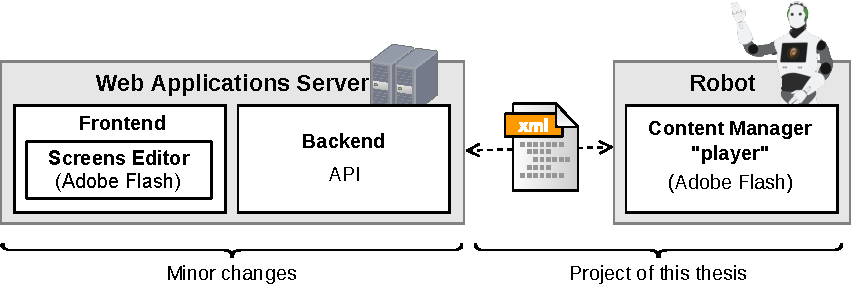
\includegraphics{figures/intro-system-overview.pdf}
    \caption{Overview of the Content Management System}
    \label{fig:intro-system-overview}
\end{figure}
More specifically, \textbf{this thesis deals with the reengineering of Flango \cm , the part of the system deployed \textbf{in the robot}} that displays content applications on the touchscreen of \reem{H} (\fref{fig:intro-system-overview}).
\textbf{It does not reengineer the rest of the system}, like the web application (that uses \flash as well) to generate content applications, although there might be minor changes to adapt their interfaces to the new technology.

It is desired not only to develop a practical solution but also to guarantee that the final output of the Flango \cm is the same that the old system generates.

This thesis is eminently a practical work, although the theoretical background has been extensively explored. 
Using web technology in a component of the robot is a novelty in the company. 
It is done to develop a sustainable product based on open standards (as opposed to the current implementation with \flash) that can be extended and reused for other robotic products that might be designed in the future.

\section{\company}
\company is a company based in Barcelona dedicated to R\&D of humanoid robots and robotic components. 
An international team of mostly mechanical, electronics and software engineers pushes forward the research on different fields, like speech recognition and generation, computer vision, walking, grasping, machine learning and navigation amongst others.
The company has developed 6 humanoid robots until 2013: \reem{A}, \reem{B}, \reem{H1}, H2 and H3, and \reem{C}.
This project targets \reem{H2} and H3, service robots with wheels and touchscreen.

\subsection*{Reem H2 and H3}
\reem{H2} (\fref{fig:reemh2}) and H3 (\fref{fig:reemh3}) are humanoid service robots featuring a screen on their torso.
They have an autonomous navigation system, speech recognition and voice synthesiser, they can find their way in different settings and help or entertain people in a friendly way.
They are intended for use in public places such as hotels, malls, airports or museums.

\begin{figure}
   \centering
   \begin{subfigure}[b]{0.4\linewidth}
       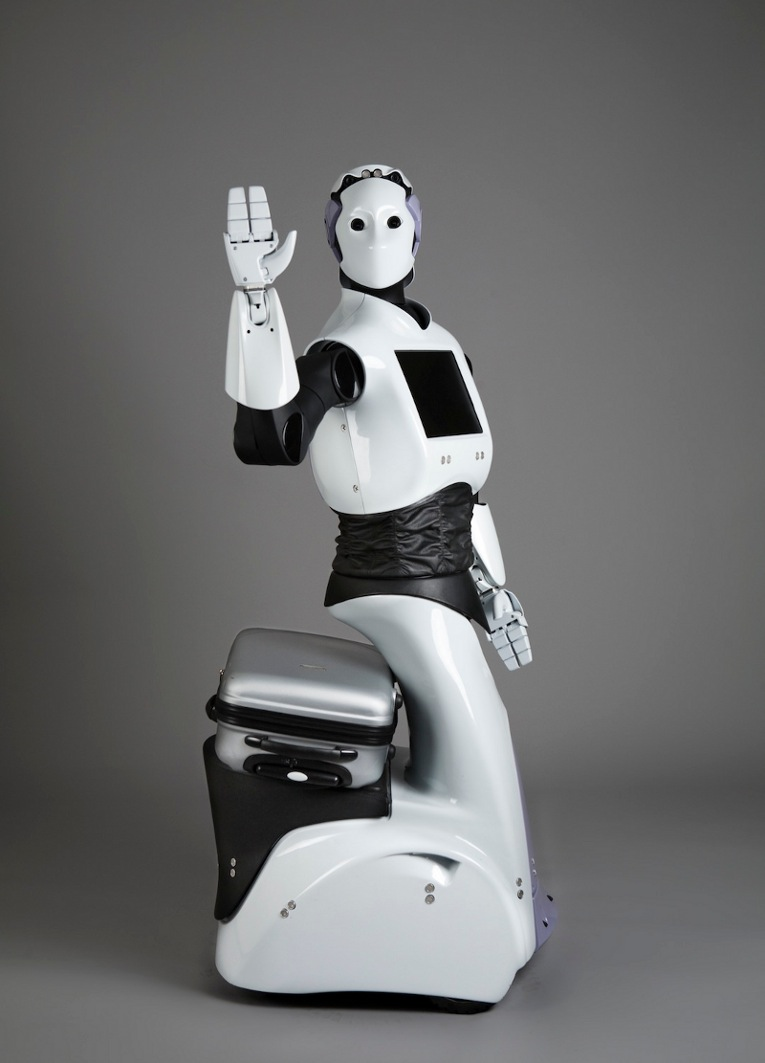
\includegraphics{figures/reemh2}
       \caption{\reem{H2}}
       \label{fig:reemh2}
    \end{subfigure}
    \begin{subfigure}[b]{0.4\linewidth}
           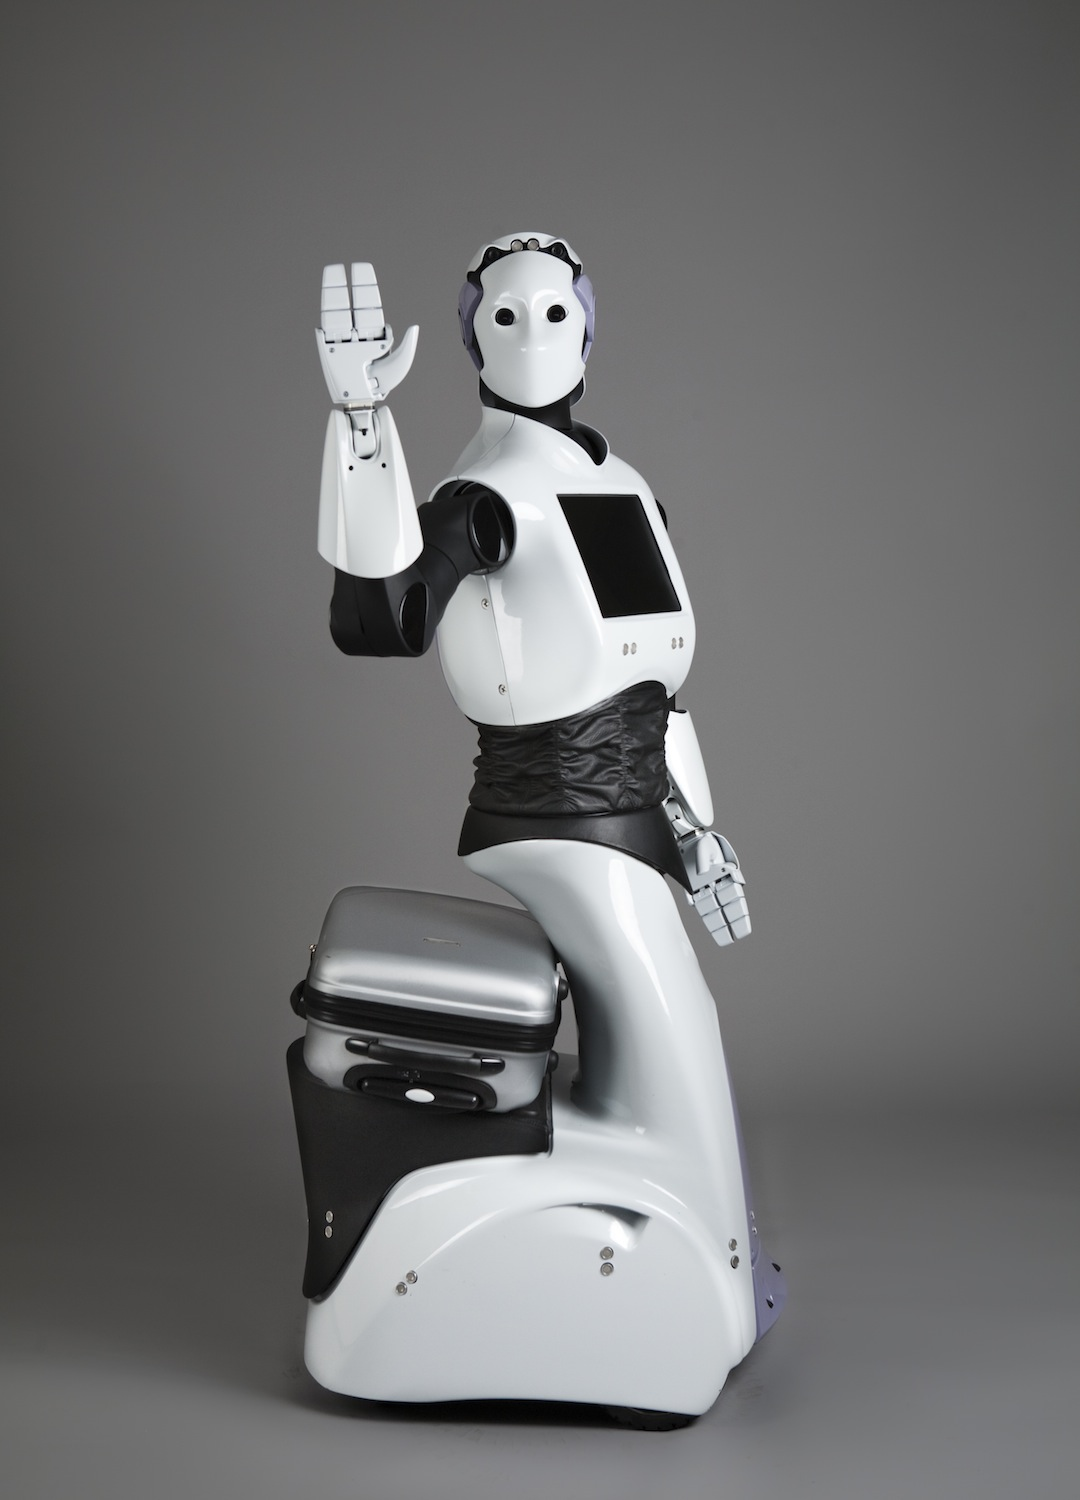
\includegraphics{figures/reemh3}
           \caption{\reem{H3}}
           \label{fig:reemh3}
    \end{subfigure}
    \caption{\reem{H} Series}
    \label{fig:reemseries}
\end{figure}
\FloatBarrier
\begin{table}
    \centering
    \begin{tabularx}{\linewidth}{| X | X |}
    \hline
    Weight & 90 Kg\\ \hline
    Height & 1.70 m \\ \hline
    Battery life & 8 h \\ \hline
    Degrees of freedom & 22 \\ \hline
    Payload & 30 Kg (mobile base), 3 Kg/arm\\ \hline
    Speed & 4 Km/h\\ \hline
    Computer & Core 2 Duo + Atom\\ \hline
    Sensors & Microphone, stereo-camera, laser, ultrasounds, accelerometers and gyroscopes\\
    \hline
    \end{tabularx}
    \caption{Reem H2 and H3}
    \label{tab:rh2}
\end{table}
\FloatBarrier
\section{The Current System}
The \reem{H} series have a multi-modal interface: besides speech or joystick manual control, humans can use a touch screen to command the robot or obtain information.
\reem{H} can display multimedia contents like videos, facts about a company, robot features, language settings, etc.

The Contents Management System comprises \emph{\flangofe} and \emph{\flangobe} (both in Basestation), and \emph{Flango \cm} (in the robot) (see \fref{fig:intro-system-overview}).
The Basestation is an application server that hosts Flango, a \ac{RIA} to manage contents and robots made with Django, a widely used framework for Python. 
Clients can create content applications  with the \flangofe (\se), a tool built with \flash .
When content applications are ready, clients can associate $1$ application with $n$ robots to display it in the touch screen.

\lstinputlisting[label=example-screen-xml,language=XML, caption={Example Screen XML}, breaklines=true]{src/example-screen.xml}

The elements of a content application (screens and entities) have an \ac{XML} representation (listing \ref{example-screen-xml}), an approach similar to popular projects (e.g. Android, NetBeans) and even, in a sense, all \acp{RIA} made with \ac{HTML}.

The Flango \cm interprets the \ac{XML} and displays the result on the screen (\fref{fig:xml-flango-view}).

A content application is essentially a set of screens, navigation, multimedia contents, and entities. 
The latter are domain objects that can be instantiated and represented in a view. 
This way a user can create an application that shows information about the company, include buttons to provide an easy way to give commands to the robot (e.g. "follow me", "shake hands"), display videos and picture galleries, etc.
All of these components are localisable:  
They can be resized, repositioned, repainted... depending on the active language.
Using other tools, clients can also associate sentences to screens and the text-to-speech system reads them aloud.

\begin{figure}[htb]
    \centering
    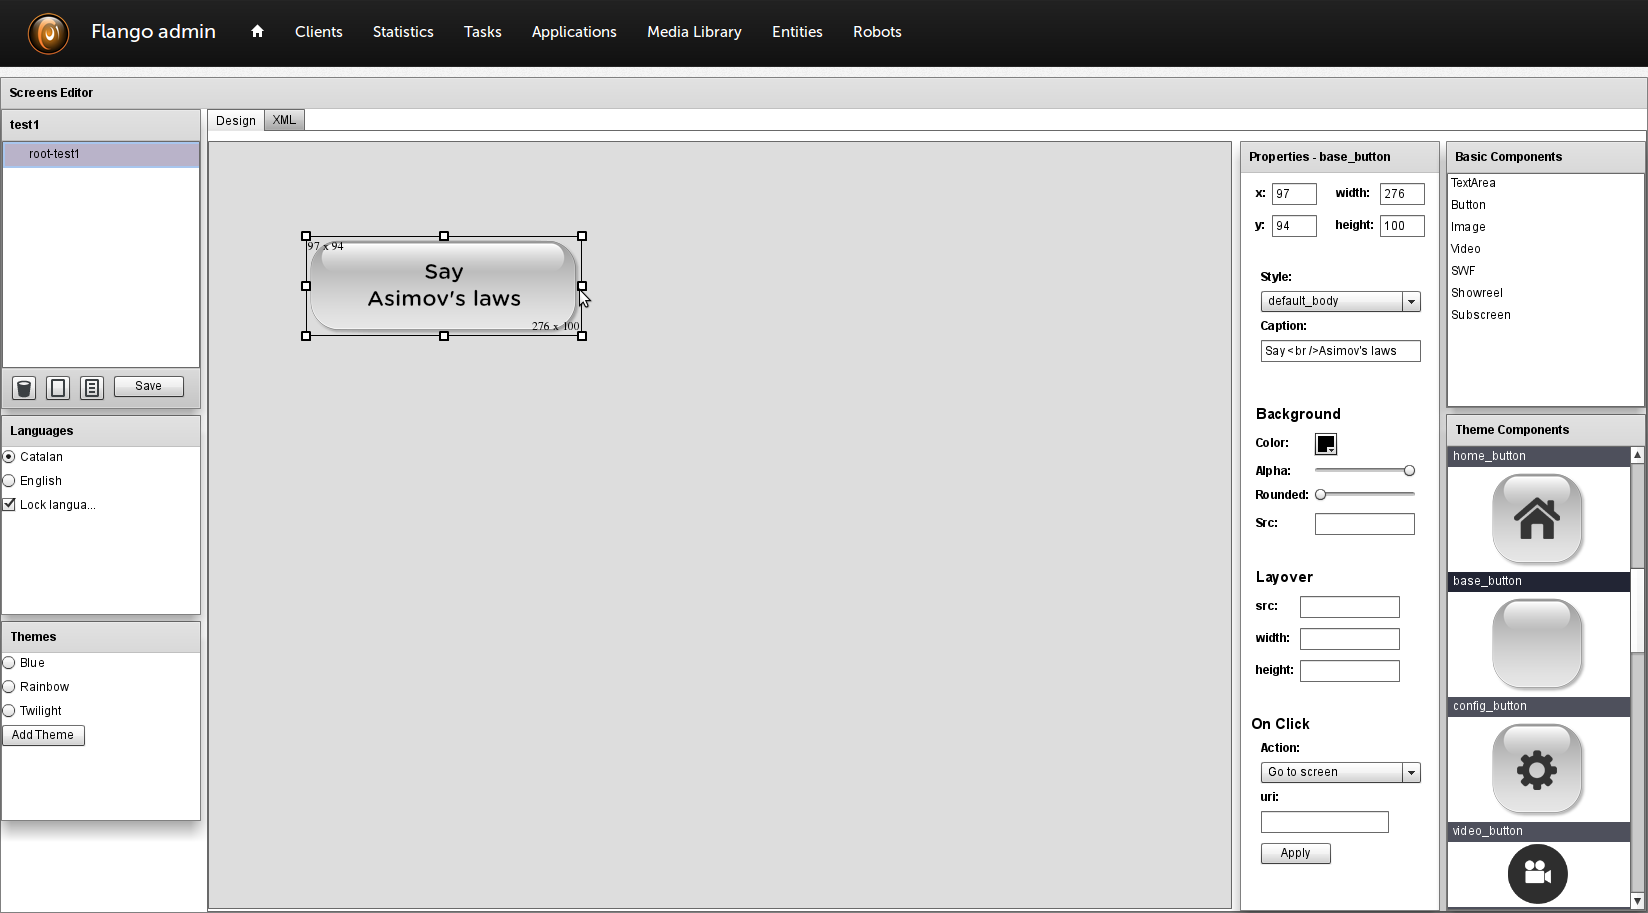
\includegraphics[width=\textwidth]{figures/screens-editor}
    \caption{\se , a \flash application in Flango}
    \label{fig:screens-editor}
\end{figure}

\reem{H} robots have a built-in software to display the content applications, the Flango \cm , which is also made with \flash .
Initially, this software has no \ac{GUI} or direct interaction with a person.
It transforms \ac{XML} files into a \ac{UI} (\fref{fig:xml-flango-view}) and, finally, displays the screens and manages the user interaction (e.g. clicks on a button).

\begin{figure}[htb]
    \centering
    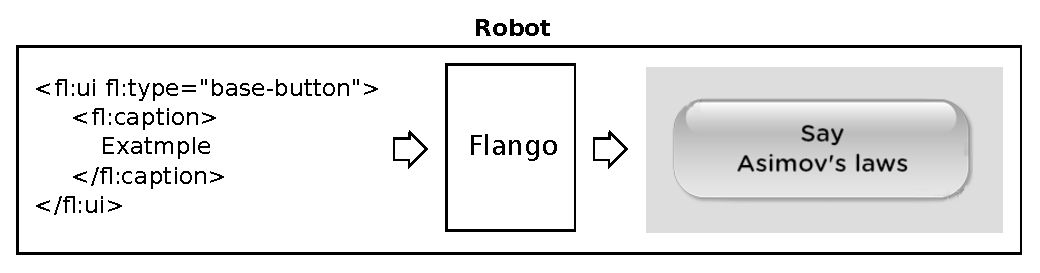
\includegraphics[width=\textwidth]{figures/xml-flango-screenshot}
    \caption{Transformation of \acs{XML} into a \acs{GUI}}
    \label{fig:xml-flango-view}
\end{figure}

\textbf{This thesis documents the project of reengineering the \cm , in the robot, with web technology instead of \flash , namely \acs{HTML5}, \acs{CSS3} and \acf{JS}}.

\section{The New System}
The \ac{WWW} was born as a document viewing platform and has evolved gradually into an application platform. 
First the web consisted of simple pages that contained structured text and some images. 
Navigation was done using simple links between pages. 
In a second phase, web sites became interactive: 
it was the time of animated graphics, browser plug-ins and JavaScript. 
More recently web sites have adopted features from traditional desktop software in \acp{RIA} \cite{Anttonen:2011}.

For a decade, the \flash player plug-in has provided a platform to enable rich and interactive content in browsers.
However, Adobe has made the updates exclusive to the Google Chrome\textsuperscript{\textcopyright}\xspace browser \cite{FlashRoadmap}. 
The browser in the robot application, QtWebBrowser, uses this plug-in but will not receive updates from Adobe. \company ' systems need to adapt to this new setting. 
There are two solutions:
\begin{itemize}
	\item Use Google Chrome instead of QtWebKit
	\item Use modern web technologies, either in QtWebKit or in another browser
\end{itemize}

The solution is rethinking the application to be a part of the robot's system and implement it with modern web technology.
There is a number of technologies that could be used, but the Web allows the product to be easily portable, very extensible, open to many developers and sustainable as it does not depend on a single company.
\ac{HTML5} is perhaps the best known forthcoming standard in the Web and is typically combined with JavaScript and \ac{CSS3}. 
It has become such a popular combination that major browser vendors provide support for the latest drafts of the \ac{W3C}, like the audio \ac{API} for \ac{HTML5} or the video support.
A big number of frameworks with JavaScript have appeared not only client-side (e.g. BackBone, jQuery, Ext JS, Google Web Toolkit, Yahoo User Interface Library...), but even server-side (e.g. NodeJS).
Moreover, new \ac{HTML5} capabilities and \acp{API} are an opportunity to add features to this project.

The project of this thesis uses Google Angular\textsuperscript{\textcopyright}, a \ac{MVC} framework that lets developers \emph{teach the browser new syntax}. 
Thus, \ac{XML} files created with the \se can be interpreted natively in a browser. 
This has some advantages over \flash \cite{Jobs:ThoughtsOnFlash}:
\begin{itemize}
    \item No use of third-party plug-ins
    \item Openness
    \item Reliability, security and performance
    \item Keeps power consumption lower (e.g. using the GPU to decode video or apply transformations and smooth transitions to elements on the screen)
    \item Touch-enabled: the new screen of Reem H3 is multi-touch. To enable gestures, heavy rewriting of the current Flash application is required.
\end{itemize}


\section{Goals}
This thesis is part of the specialisation of \emph{Software Engineering and Information Systems}. 
The goal is to reengineer the Flango \cm with web technology.
More specifically, the author has to gather the requirements from an existing system, plan in terms of scope, time and cost, make the system specifications, design and implement it using modern web technologies, use quality assurance tools and deploy it successfully in a \reem{H3} robot.

Regarding the project, the goals are:
\begin{itemize}
	\item Reengineer the current system with web technology
	\item Develop a testing strategy to make it robust
	\item Make it compatible with non-reengineered parts of the system
\end{itemize}


\section{Organisation of This Document}
This document describes the system developed at \company to display the  content applications created with the \se on the \reem{H} series.
It does not cover other software on the robots or in Basestation.

This document describes the project as follows:
\begin{description}
\item[Related Work] Provides a general overview of topics surrounding those of this thesis, enabling for a deeper understanding of the material at hand.
It starts with a description of the reengineering process, followed by a section about web technology and, finally, a description of the methodology of the project -- \ac{TDD}.

\item[Project Management] Contains information about the project from the point of view of management. 
Detailing on schedule, budget and risk analysis. Contains an assessment of the execution.

\item[Requirements] States the functional and non-functional minimum requirements, the constraints and weights the use of off-the-shelf solutions.

\item[Specification] Defines what the application does in the context of a reengineering process. 
It deals with the first three steps: a software inventory, documentation restructuring and a description of the current system (with special attention to context, interoperability and interaction).
Contains the specification of the new system: a conceptual model, use cases and the behaviour model, with sequence diagrams and contracts of system operations. 

\item[Design] Describes the internal design of the software in the context of a reengineering process. 
It contains the last three steps: code restructuring, data restructuring and forward engineering.
Detailing about the system architecture and the context and the patterns used.
Contains a static view (class and packages diagram), a dynamic view (sequence diagrams) with examples of the most relevant operations and a physical view (deployment diagrams).

\item[Implementation] Holds technical details about the environment, the set-up, the integration in the robot and a larger system and meaningful examples of the technology used. 
Emphasises the implementation of the patterns described in previous chapters.

\item[Testing] Highlights the strategy to implement tests and the integration in the robot system.

\item[Conclusion] Presents the conclusions from technical, academic and personal point of view. 
Includes challenges faced during developments and future work. FIXME

\item[Appendix A] Lists UI Components of the old system.

\item[Appendix B] Lists unit tests that define the behaviour of most components of this system.

\end{description} % intro
\chapter{Related Work}
This chapter is a short introduction to the main knowledge areas involved in the development of this project.
It describes what has been done before in the field and the theory the project is based upon.
It includes the motivation and the steps to reengineer an application , the evolution of web technology from simple documents to \acp{RIA} like the one of this thesis, the \ac{TDD} method and the relationship with \ac{DbC} and, finally, \ac{XML} as an intermediate representation of the model to interoperate between Basestation and Flango \cm in the robot.

\section{Reengineering}
\label{sec:reengineering}
This thesis takes over the work of the past two years at \company in content management.
The initial situation is a system made with \flash and Django called Flango.
The \se and the robot's \cm are \flash applications.
Whereas the first one runs in a modern browser, on desktop computers, the robot's \cm runs in the robot.
The robot is a Linux system and the browser is a QtWebKit widget embedded in the Qt application that governs the hardware.
The \flash plug-in will not be updated and this part of the system has to be rewritten in a different technology.

\begin{quote} 
Consider any technology product that has served you well. 
You use it regularly, but it's getting old. 
It breaks too often, takes longer to repair than you'd like, and no longer represents the newest technology.
What to do? If the product is hardware, you'll likely throw it away and buy a newer model.
But if it's custom-built software, that option may not be available. 
You'll need to rebuild it. 
You'll create a product with added functionality, better performance and reliability, and improved maintainability.
That's what we call reengineering. \cite{Pressman:2007}
\end{quote}
Unlike other products, software does not degrade with time due to external factors such as the inclemencies of the weather, power outages or intense use.
Software packages are adapted, corrected, extended and improved constantly.
That can lead to unstable applications or unexpected side effects, even if the original product had been designed with the best practices at that time.
After a certain amount of time, changes are harder to implement. % FIXME language
Sometimes the vendor of frameworks, libraries and third-party software used in a project stops supporting it and the only solution is substituting the components that depend on it. 
The product becomes unmaintainable in many aspects and reenginering is required. 

Software reengineering comprises \textbf{6 activitie}s: \textbf{inventory analysis}, \textbf{document reestructure}, \textbf{reverse engineering}, \textbf{code restructuring}, \textbf{data restructuring} and \textbf{forward engineering}.
Simple put, it is all about understanding the current logic of a program and modifying the three typical components: data, logic and view.
The project of this thesis is not modifying the current program but developing a new one with new technology, focusing on reverse engineering the original software. 

Doing an inventory of the software that belongs to the system is part of the definition of the project scope.
Making a list of programs with the current status, dependencies and physical location helps on getting an overview of the project.
Usually software has documentation that needs to be added to the inventory and, sometimes, restructured.
After this, the reverse engineering process can start.

\paragraph{Reverse Engineering}
Three dimensions drive tasks in the reverse engineering activity (FIXME task in activity or the other way round?): abstraction level, completeness and directionality.
To understand what the software does, abstraction should be as high as possible.
This information can have many details or not (completeness) and can be created in one way (extracting it from the source code) or two-way (feed information to the reengineering tool).
This project does not use any computer-assisted reengineering tool.

\subparagraph{Understand current program}
A program normally has input data, logic that processes it and a view:
The first activity is understanding the processing.
Code can be examined at several levels of abstraction: system, program, component, pattern, statement.
Some key aspects include the interaction, interoperability or the context.
Data structures, classes, schemas in databases, etc have to be identified and possibly redesigned in the next steps.
Finally, the \ac{UI} has to be analised as well. 
There are issues related to presentation of data, interaction, usability, etc that have to be identified.
This project focuses on system and program levels of abstraction and on interoperability.
The software does not have any views or databases to be reconsidered.
However, it does have some formats server-side (in the backend) that are candidates in this process (e.g. definition of settings with \ac{XML} might have to become \ac{JSON} or have a different structure).

\paragraph{Restructure code and data}
Sometimes the solution is restructuring the current program.
The project of this thesis skips this part because a new application is being developed using the output of the first activity (FIXME: activity?): understand the current program
Restructuring the code might not be enough in most cases. 
It can fix immediate issues but it is not a long-term solution.
However, when doing so, \ac{TDD} is useful because tests breaks immediately and often, specially if they are running in the background or periodically.
To improve the software design both data and architecture should be restructured.
\ac{TDD} can provide robustness to this process: if there are tests available, the new design can be proven to work, at least, for the example cases. 
If not, the solution can be built incrementally with tests that define the requirements of the system (extracted in the first activity (FIXME: activity?), thus using them as an specification.

\paragraph{Forward engineering}
There is a number of options when it comes to apply changes in the current program. 
For example, apply patches, redesign parts of the software or completely redesign it.
Depending on the circumstances, completely redesigning a software might be costly but, in the long-term, it might be a cost-effective solution.
The project of this thesis is redesigning the software to incorporate new practices, new technology and, in the future (out of the scope of the thesis), additional requirements.
The outcome of this process (FIXME process vs activity vs task) is a new software that replaces the current implementation.

%introduction

%software reenginering:
%main activities (software reengineering prcess model defines 6 activities, fig 30.2):
%inventory analysis
%document reestructure (option 1)
%reverse engineering
%code restructuring
%data restructuring
%forward engineering

%reverse engineering:
%keys: abstraction level, completeness, directionality:
%abstraction: make it as high as possible (ideally, entity-relationship models)
%completeness: how much detail prvided at an abstraction level?
%(there are tools to analyse software but this thesis isn't using them)
%directionality: one way. extract info from the source code, give it to an engineer, use it during any mmaintenance %activty,. it can also be two-way (feed info to a reengineering tool that fixes the old program)

%first activity of reverse engineering: understand processing. analyse code at varying levels of abstraction: system, %program, component, pattern, statement. 
%understand overall functionality before doing more steps (set a context, pay attention to interoperabilty issues). %Block diagrams of the programs (show interaction). do some narrative for each component.
%normally there is code for: prepare data, process data, prepare results for the view

%next activity: understand data:
%internal data structures. goal: identify classes. focus on teh definition of classes of objects. book is old-fashioned %and assumes crappy old code.
%database structure. bottomline: rethink the design.

%next: reverse enginer UI

%restructuring
%(mention it. this is related to TDD)
%code restructuring is not enough. it alleviates immediate problems. real benefit is achieved only when data and %architecture are restrucured. spaguetti-bowl code to structured programming.
%data restructuring: standarise, rationalise, make physical modifications.

%forward engineering: change the code, redesign, or make big changes (completely redesign, recode, test..). preventive %maintenance. cost of maintenance.


\section{Web Technology}
% quotations: something about emacs life style, or berners lee
The \ac{WWW} plays a central role in many people's lives.
The first drafts date back to the 1980s, the first web browser prototype by Tim Berners-Lee was built in December 1990 and the Mosaic browser was completed in 1993.
After that, Netscape, Mozilla Firefox, Microsoft Internet Explorer, Google Chrome, Safari, Opera, Konqueror and many other browsers appeared, along with some nowadays popular websites (e.g. Amazon, 1995).

For many people the browser is the most used application in many devices. 
The web creates opportunities and makes documents accessible like tax records, maps, banking information, phone directories or product catalogues.
New business models, like new ways of promoting products, selling music or movies, are developed having the web as a core part.
Innovation goes beyond all these with experiments and products like FirefoxOS or ChromeOS to build an operating system where the web is the main development platform.
Other companies, like Citrix or eyeOS, offer web applications or virtualisation tools that resemble an operating system %\cite{Gamonal:2011}.

%goals: explain evolution of web tech, state of the art, and why it is better than flash.

%* programs in browsers. isolate them? flash plugin. flash is dead (jobs or other
%articles) 
%* browsers: architecture (dom, js engine, html renderer...) from mosaic to
%%fx/ch/qtwebkit 
%** webkit and qtwebkit
%
%* client-side tech: JS, css, html/xml 
%** evaluation and comparison 
%** frameworks
%
%browsers, JS engines, chrome v8, fx gecko, QtBrowser
% functionaliyy (interoperability, security), reliability (maturity), usability: (learn-
%ability, attractiveness) Efficiency: (time behavior, resource utilization) Maintainabil-
%ity: (stability) Portability: (installability)

\subsection{From Plain Documents to Applications}
\paragraph{The Evolution of the Web}
\begin{quote} 
HyperText is a way to link and access information of various kinds as a web of nodes in which the user can browse at will. 
Potentially, HyperText provides a single user-interface to many large classes of stored information such as reports, notes, data-bases, computer documentation and on-line systems help\cite{BernersLee:1990}
\end{quote} 

When the \ac{WWW} was started in 1990 it was intended to be a document viewing platform.
It has evolved in at least three phases \cite{Anttonen:2011} \cite{Taivalsaari:2008}:

In the early days, websites were basically a few files with plain text, forms and page-structured artifacts, possibly static images and hyper-links (anchors) to provide navigation. 

Later on, browsers added programming capabilities, plug-ins and allowed animated graphics. 
Web pages became interactive and client-server communication increased in complexity.
\flash (at that time Macromedia Flash), ShockWave, Java, QuickTime and a few others allowed the inclusion of multimedia contents or even programs (e.g. Java Applets).
Engineers could combine server-side and client-side technology to provide some more capabilities along with content.

More recently, despite the fact that the web browser was not designed for running applications, since 2008 users have headed this way. 
In this third phase, web pages are not just documents: they have complex user interaction capabilities, they do not require full page refresh and typical use cases have evolved. 
A big part of applications is executed client-side, taking advantage of the computing capabilities of modern hardware and decreasing the load in servers. 
In some cases, the application also needs huge server-side resources and uses strategies like cloud computing (e.g. Amazon EC2) to scale up.
Today the web is not only about viewing documents but about world-wide sharing, collaboration and interaction, possibly in real time. 

Web browsers have become a widely-used platform for software applications. 
Video editors, spreadsheets, calendars or 3D games used to run exclusively on desktop computers. 
Today, they run in a variety of devices and some of them even do it in a browser. 
There are 3D engines ported to Web, real time collaboration, full HD video support without plug-ins and many more features built-in a system, the browser, that is not an ideal execution environment for desktop applications.

\paragraph{\ac{RIA}}
\acp{RIA} are neither web services or web pages. 
They are software systems based on technologies and standards of the \ac{W3C} that provide web specific resources such as content and services through a web browser \cite{Kappel:2006}.
Typically one designs them as single page websites.

% FIXME language
Web applications differ between them. 
They can be document-centered, workflow-based, portal-oriented, collaborative, social, etc. 
They all have some common characteristics. 
Amongst others:
\begin{itemize}
    \item The product
    \begin{itemize}
        \item Content is the core.
        \item Hyper-text: non-linearity is a main distinction to traditional software systems. There are many ways of landing on a certain page. This can lead to disorientation or cognitive overload for users.
        \item Presentation aesthetics, usability and interaction are closer to a desktop application than to a web page
    \end{itemize}
    \item Use
    \begin{itemize}
        \item Globality: Spontaneity and multiculturality of users. Web applications are publicly available.
        \item Quality suffers from unknown network characteristics
        \item Multiplaform delivery involves having different devices, browsers and degrees of functionality and performance
        \item Intense network usage. Remote calls are minimised. The use of software patterns like remote facade, remote proxy, \ac{DTO} or \ac{RPC} is frequent
    \end{itemize}
    \item Evolution
    \begin{itemize}
         \item Continuous change
         \item Competitive pressure
         \item Fast pace development
    \end{itemize}   
\end{itemize}

The project of this thesis is, in a sense, both a \ac{RIA} and a \acp{RIA} generator. 
It is a \ac{RIA} because, among other reasons, it works in the browser with web technology and has an intense use of the network to fetch the model or other components to build the screens.
The rendered application works in a browser, has an intense use of the network as well and is content-centered.
Despite the fact that it works in the specific content of a robot, globality is still an issue.
A typical scenario would be a fleet of robots in a conference: users from many different cultural backgrounds can use the application at any time.


\subsection{Browsers and isolation of programs}    
Many of the websites in the aforementioned third phase contain substantial amounts of client-side code. 
At the end of the day, a \ac{RIA} is a distributed software. 
In the past the client-side part was thin and simple, whereas today's application have complex logic delegated to client nodes with local storage, hardware-accelerated components, websockets and other advanced capabilites.

In spite of the fact that \acp{RIA} have grown in complexity and now demand more resources, browsers architectures still do not provide sufficient isolation between concurrently executing programs.
A similar problem occurred in early operating systems (e.g. MS-DOS), before processes appeared \cite{Reis:2009}. 

Most of browsers have a monolithic architecture with poor isolation between web application instances. Chromium, however, implemented an architecture based on \ac{OS} processes. 
Another way of isolating web applications is running them in a plug-in container. 

The project of this thesis does the first phase with Qt WebKit, the port of WebKit on top of Qt, to display the application in a Qt dialog and communicate with the hardware. 
The second part uses Chrome to meet the technology requirements.
Qt WebKit components comprise the WebCore and SquirrelFish Extreme, which compiles Javascript into native machine code. 
It is compatible with Adoble Flash Player but because it will not receive more updates in the future, it will not be used any more.
The \flash plugin is a black box isolated from other elements in the \ac{DOM}.
Isolation is not an issue in this project because there is only one application running at a time and, even in a normal use of a browser, with many websites running at once, isolation is not a blocking issue.
FIXME MAYBE ADD CHROME V8 engine, ETC.

% MOVE THIS TO DESIGN
%\section{Client-side Technology}
%The software of this thesis is developed mainly on the client side and is part of a Web system.
%There is a number of technologies to develop applications client side. 

%\subsection{Comparison of languages}
%\subsection{Frameworks}

\section{Test-Driven Development}
The software written for this thesis is executed in a complex environment.
Testing it properly and ensuring the quality is crucial to avoid unexpected behaviour in one of the most visible parts of this system, the screen.
Crashes and \ac{UI} flaws can lead to triggering wrong external calls to other components of the system (e.g. displaying a Qt dialog different than expected, not making the call, sending it with bad parameters...), blocking access to features or seriously affecting the \ac{UX}.

Reengineering this system has, at least, two sources of potential errors: 
undocumented features in the original application (unknown, documented wrongly, partially documented or not described at all) and integration of the new software in the current system.

% maybe put all this in a table?
\ac{TDD} is based on having numerous and very short iterations with these steps:
\begin{enumerate}
    \item Add an initial (failing) test
    \item Run all tests and see if the new one fails
    \item Write the minimum amount of code to pass the test
    \item Run the automated tests and see them succeed
    \item Refactor the code. Conform to standards and best practices
\end{enumerate}

As opposed to classic development methodologies (e.g. waterfall, where tests are done in the last place), with \ac{TDD} tests go first. 
Specification and documentation of the system are not artifacts created before the implementation but the tests themselves.

Testing earlier and heavily has benefits over the classical approach:

\textbf{Efficiency} Defects (and their causes) are identified earlier.

\textbf{Robustness} The system is more reliable and stable. 
The \ac{QA} process is easier to maintain and much more strict.

\textbf{Maintainability} Small fixes can introduce new errors in the system. 
Testing continuously and producing the minimum amount of code to implement a feature reduces this.

\textbf{Extensibility} \ac{XP} embraces change. 
It is easier to adapt to changes in the requirements. 
This thesis is reengineering a project that is not frozen. 
During the development, the original software keeps adding features and bug fixes.

This methodology is specially useful in the implementation of this project for two reasons: 
the Google AngularJS framework is extremely friendly with unit testing and \ac{E2E} tests thanks to Karma Runner, and the company has the infrastructure to incorporate the project in a continuous integration system with Jenkins.

\section{XML as an intermediate representation}

lorem ipsum
 % related work
\chapter{Project Management}
This chapter describes the planning of this project in terms of scope, schedule, cost and risk.
The execution and deviations are shown at the end of this chapter.

\section{Scope}
\label{sec:scope}
The system has three parts: the \flangobe, the \flangofe (with the \se) both at Basestation, and the screens renderer in the robots (the robot's \cm \fref{fig:system-overview}).

\begin{figure}[htb]
    \centering
    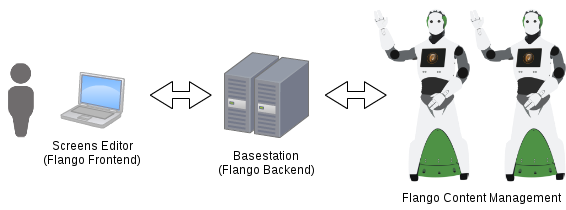
\includegraphics[width=14cm]{figures/intro-system-overview}
    \caption{System components}
    \label{fig:system-overview}
\end{figure}

This project reengineers the robot's \cm with web technologies but not the back-end and front-end, that remain in Django and \flash.
The input of the new \cm are contents applications, generated with the \se . The output is the screen rendered with web elements.
Contents applications have configuration files that define the theme, the location of binary resources (images, videos, etc), the default language and other settings. 
This project can read and use the configuration files.
This project accepts valid syntax generated with the \se for a comprehensive set of components (\texttt{back-button}, \texttt{base-button}, \texttt{image}, \texttt{video}...) and their properties (\texttt{width}, \texttt{x}, \texttt{y}, \texttt{background}...), and generates \ac{HTML5} that renders them as defined.

Developing an intense testing strategy is part of this project.
The final artifact is this master thesis that describes the system and the rationale that guides all decisions.

\section{Schedule}
This project has 4 phases that match the 4 typical groups of processes: initiating, planning, executing (and monitoring + control) and closing.
The execution has 3 deliverables: viability and proof of concept, iteration 1 (basic program) and iteration 2 (extended program).

\subsection{Phase 1: Initiating}
\paragraph{April, 1 -- April 4}
The initiating processes determine the goals of the project and the scope.
This stage was partially done before the beginning of this thesis to ensure its viability in the company.
It was agreed that the project would reengineer the current system using web technologies (see \fref{sec:scope})

\subsection{Phase 2: Planning}
\begin{sidewaysfigure}[htb]   
    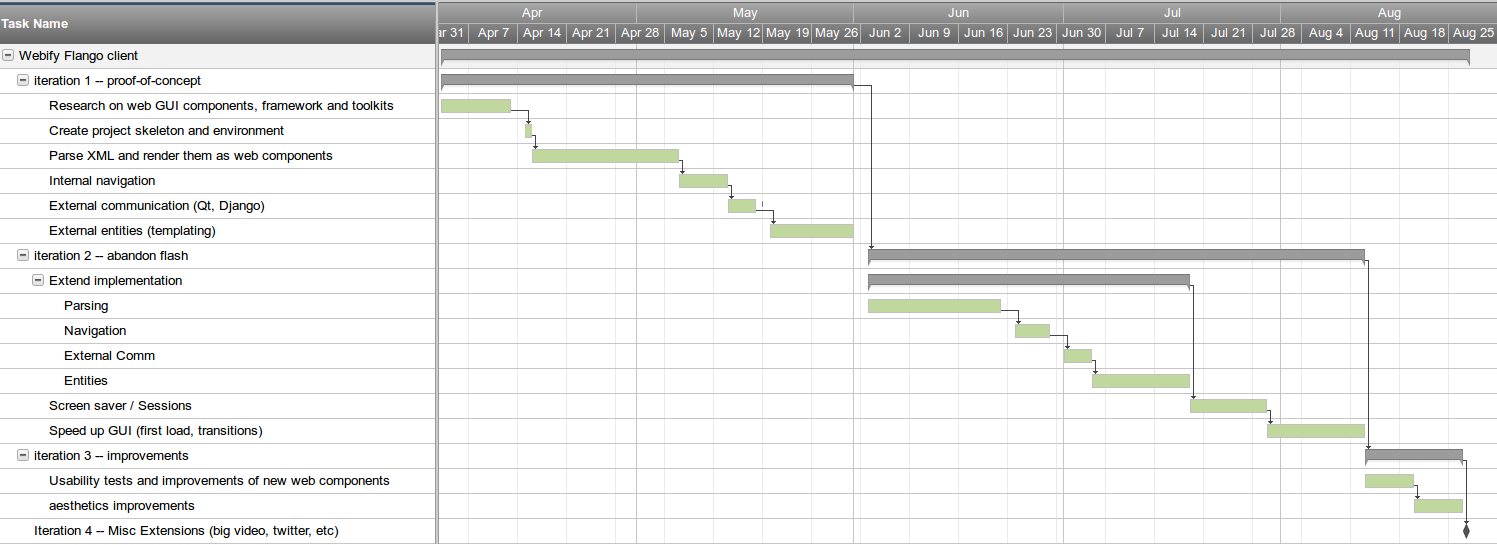
\includegraphics[width=\textwidth]{figures/plan-gantt-orig}
    \caption{Original Gantt Chart}
    \label{fig:plan-gantt}    
\end{sidewaysfigure}

\paragraph{April, 5 -- April 6}
The first draft of the plan is a rough estimation of the tasks length and a definition of the big milestones.
Because there is only one engineer there are no concurrent tasks and free floats are always zero.
Other activities of this phase include an estimation of the resource requirements for upcoming tasks, developing the budget (\fref{sec:budget}) and risk planning (\fref{sec:risk}).
See the Gantt chart in \fref{fig:plan-gantt}.

\subsection{Phase 3: Execution}
\paragraph{April, 7 -- August 28}
The execution phase focuses on building the product. 
A web engineering process should be incremental, with frequent changes and short iterations \cite{Kappel:2006}.

\begin{table}[htb]
    \centering
    \begin{tabular}{| l | p{11cm} |}
    \hline
    Milestone & Deliverables \\
    \hline
    Proof of concept & Research on frameworks and tools to develop the project. Choose one. Build a minimal working example to illustrate key aspects of the project. \\ \hline
    Iteration 1 & Build a prototype comprehensive in number of features but simple in the implementation to validate the technology. \\ \hline
    Iteration 2 & Extend the prototype of Iteration 1 to complex cases. \\
    \hline
    \end{tabular}
    \caption{Milestones and deliverables of the execution phase}
    \label{tab:milestones}
\end{table}

This phase has 3 big milestones, one per iteration (\fref{tab:milestones}). 
The outcome of each iteration is a product with a set of stable features and the corresponding unit tests which, in turn, serve for the purpose of documentation.

\subsection{Phase 4: Closing}
\paragraph{August, 29 -- September 14}
Prepare package with a stable set of features, presentation and documentation.

\FloatBarrier

\section{Cost}

\FloatBarrier

\label{sec:budget}
The estimated length of the project is $105 days \times 8 \euro{} \times 8 hours = 6720 \euro{} $

\begin{table}[ht]
    \centering
    \begin{tabular}{| l | l |}
    \hline
    Labour & 6720\euro{} \\ \hline
    \multirow{3}{*}{Hardware} 
        & Desktop Computer (amortized) 250\euro{} \\ % check this
        & 22 Monitor (amortized) 50\euro{} \\
        & Reem H3 testing time 150\euro{} \\ \hline   
    \multirow{2}{*}{Software}
        & JetBrains WebStorm license 89.10\euro{} \\ % check this    
        & GNU/Linux 0\euro{} \\ \hline
     Overall & 7259.10\euro{} \\ 
     \hline
    \end{tabular}
    \caption{Budget}
    \label{tab:budget}
\end{table}

There are some infrastructure related costs excluded from the budget because they are part of the office maintenance monthly expenses.
This is the case of subversion servers, network, power, backups, etc. 

\section{Risk Analysis}
\label{sec:risk}
\begin{risk}
{Schedule: deviation}
{There might be urgent needs in the company, like demos to potential customers or hot bugs related to contents applications}
{Some of the needs are unpredictable. However, preventive maintenance and good documentation of bugs in tickets can reduce the chances that this risk will occur.}
{Do the urgent task and reschedule the project}
\end{risk}

\begin{risk}
{Resources: deviation}
{The engineer might have to dedicate resources to other tasks in the company non-related to this project.}
{Coordinate action monthly with the managers and track deviations and progress weekly. Avoid dedicating less than 50\% of time to this project.}
{Limit scope and extend deadlines to have the expected number of hours dedicated to this project.}
\end{risk}

\begin{risk}
{Resources: infrastructure crash}
{The development system might die}
{Use version control systems and do frequent and small commits. Delegate backups to the IT team.}
{Restore backups}
\end{risk}

\begin{risk}
{Resources: testing environment not available}
{Most of the testing can be done with regular computers. However, final tests have to be conducted with real hardware: ReemH3-1 or 2 and Reem-H2, which are frequently booked to go on tour, perform shows, demos or development.}
{Book 3 days in advance if testing is critical. }
{Share the robot with a team that doesn't need the media computer of the robot, where this project is hosted.}
\end{risk}

\begin{risk}
{Personnel: Application expert leaves the project}
{There is only one application expert that can leave the company. Nobody else has advanced knowledge on the internals of the current implementation.}
{Build a common agenda with the expert and document critical and complex parts of the current application. Find experts in similar technology in the team}
{Reach him on-line, hire him as consultant, take conflicting features out of the scope of the project.}
\end{risk}

\begin{risk}
{Quality: critical use cases not implemented}
{One or more critical use cases can not be implemented}
{Verify that the technology allows implementing them. Build a prototype. }
{Find a workaround. Assess the importance of the affected use cases and adapt to change: decide if changing the specification of the use case will fix this.}
\end{risk}

\begin{risk}
{Quality: look and feel of the current theme can't be implemented}
{The current look and feel and interaction is designed for Adobe Flash. It might not suit the way web technology works.}
{Verify that the technology allows it with a prototype.}
{Change the external design to balance the needs of the technology and the customer}
\end{risk}

\begin{risk}
{Scope: Non-intuitive implementation with web technology}
{Current implementation is designed for Adobe Flex. Some of the use cases to implement might not fit well with the new technology}
{Analyse and discuss use cases with the author of the old implementation}
{Explore ways to change the implementation of the use case in the Screens Editor (which generates the input for the new program) to fit in the new design}
\end{risk}

\begin{risk}
{Inadequate technology}
{The chosen technology is inadequate: it doesn't allow a complete reengineering of the application (100\% of chosen use cases), performance is more than 10\% lower, it is not reliable and fails in more than 3\% of action executions}
{Assess at least 2 solutions before implementing a prototype. Implement a prototype with basic cases of at least each critical feature.}
{sdnsdgndf}
\end{risk}

\begin{risk}
{Tool: Flango or \se do not perform as advertised}
{The current implementation of the backend or the screens editor might have bugs.
Some undocumented features or \ac{XML} elements might be misleading (e.g. The normal behaviour for the QR component is generating a QR code. \lstinline$<ui type="qr" src="path">$ does not generate a QR code, but embeds an image that already exists instead.) }
{Contact the application expert before implementing the feature.}
{Fix the backend (python) or ask/hire the application expert to fix the screens editor (Adobe Flash)}
\end{risk}

\begin{risk}
{AngularJS or dependencies do not perform as advertised \footnote{Added after specifications were defined}}
{The chosen framework and libraries have young maturity and might contain bugs, be subject to rapid changing cycles and new versions might break older versions}
{Use stable versions}
{Investigate the bug, isolate it, create a minimal full working example and, if possible, open a pull request with a fix in Github or notify the error to the project managers.}
\end{risk}

\FloatBarrier

\section{Execution}
progress, deviations, final cost
FIXME % project management
\chapter{Requirements}
Requirements can be gathered using interviews with customers, users and stakeholders, with observation, questionnaires, prototyping or even from an existing application.
In this project requirements are obtained mainly from the current implementation of the software (\fref{sec:reengineering}) and from interviews with the developer of the old version.
Some features, either deprecated or with low priority, are left out of the requirements list due to time constraints. 

\section{Functional requirements}

\subsection{Ready-made solutions}
Because this is a very specific software, there are no off-the-shelf solutions available that meet the requirements of the project.
However, there are libraries and frameworks that can be reused:

\begin{enumerate}
    \item JavaScript frameworks
    \begin{itemize}
        \item \ac{MVC}: AngularJS, Spine, Ember.js, Knockout.js, Sprout, Google Closure
        \item Oriented to Web Components: AngularJS, Polymer
        \item BackBone.js
    \item Testing: Jasmine, qUnit, phantomJS   
    \end{itemize}
    \item JavaScript libraries
    \begin{itemize}
        \item jQuery and plug-ins: Bigvideo.js, jQuery-ui, jquery-mobile , jquery-kinetic  
        \item Hammer.js, jGestures , iScroll, swipe.js
    \end{itemize} 
    \item \ac{CSS} Tools: LessCSS, SASS
\end{enumerate}

\subsection{Constraints}
Certain constraints were defined before the beginning of the project:
\begin{enumerate}
    \item Technology: the project has to be implemented using modern web technologies (\ac{HTML5}, JavaScript, \ac{CSS}).
    \item Legal: It has to be ready to be open source
\end{enumerate}

\subsection{Functional requirements}
\begin{enumerate}
    \item \textbf{Render \ac{UI} Components with \ac{HTML}}. \ac{UI} components, currently defined with \ac{XML}, have to be eventually transformed to \ac{HTML} so that a browser can render them.
    \begin{enumerate}
        \item Support for \textbf{multiple languages} via the parameter \texttt{lang}.
        \item \textbf{Components} 
        \begin{enumerate}
            \item \textbf{Basic components} \texttt{screen}, \texttt{subscreen}, \texttt{textarea}, \texttt{img}, \texttt{button}, \texttt{video}, \texttt{showreel}, \texttt{swf}, \texttt{layout}, \texttt{qr}.  Exclude: \texttt{group}, \texttt{group\_button}.
            \item \textbf{Theme components}.
            \item \textbf{Properties inline or in tags}. \texttt{x}, \texttt{y}, \texttt{width}, \texttt{height}, \texttt{scrolly}, \texttt{scrollx}, \texttt{loop}, \texttt{loopy}, \texttt{loopx}, \texttt{src}, \texttt{style}, \texttt{caption}.
            \item \textbf{Action} properties \texttt{onclick}, \texttt{onload}, \texttt{action}, \texttt{param}.
        \end{enumerate}
        
    \end{enumerate}
    \item \textbf{Themes}. The current version has a default theme, a set of \ac{UI} components that extend the basic ones and provide a certain look and feel. All theme components are eventually implemented with a basic component, e.g. a \texttt{back-button}, a \texttt{home-button}, a \texttt{base-button}, etc.
    \item Internal \textbf{navigation} (subscreens). Subscreens are containers whose content is determined by the \ac{URL}.
    \item \textbf{Settings} management. There are three configurations to load: generic settings (default language, paths...), application specific settings (current language, current theme...) and structure of the application (a graph that defines an id and a \ac{URL} for each node (screen)). FIXME: graph? not a tree definitely
    \item Basic support for \textbf{Entities}.
\end{enumerate}

\section{Non Functional Requirements}
FIXME: add measurable stuff
\begin{enumerate}
    \item \textbf{Target browser}: QtWebKit (Qt 5.0.x) for the first phase, Google Chrome 28 for the second.
    \item \textbf{Extensibility}: The software has to be extensible. The design has to allow adding new features in the future.
    \item \textbf{Robustness}: the software has to be reliable and has to be delivered with a comprehensive test suite. It should be compatible with Jenkins and continuous integration.
    \item \textbf{Hardware}: the software has to perform smoothly in Reem H3 and a multitouch screen.
    \item \textbf{\ac{UX}}: the time to change to another screen in the rendered contents application should be less than 0.5s. Media contents (images, videos) have to be ready in less than 1s after a screen change. Rendered components should be aesthetically pleasant.
    \item \textbf{Interoperability}: it has to interoperate at least with:
    \begin{itemize}
        \item \textbf{Backend}: there is an \ac{API} in a Django backend that provides settings and serves the contents
        \item \textbf{RobotBehaviour}: the Qt program that runs in the robot and governs the behaviour. Sometimes the touchscreen displays Qt windows, sometimes it displays the application contents. 
    \end{itemize}
\end{enumerate} % requirements
\chapter{Specification}
The specification of the program defines \textbf{what it does} rather than how.
This chapter presents the specification of the system taking into consideration general software engineering principles, the models proposed by Larman  in \cite{Larman:2004} (at least conceptual, use case and behaviour models) and Meyer's (FIXME CITE??) \ac{DbC}.
For the particular case of this thesis, the specification takes into account reengineering principles and procedures and \ac{TDD} as a tool to define what the system does as opposed to a simple testing technique.

Reengineering software comprises 6 activities (\fref{sec:reengineering}): 
\begin{enumerate}
    \item Inventory Analysis
    \item Documentation Restructuring
    \item Reverse Engineering
    \item Code Restructuring
    \item Data Restructuring
    \item Forward Engineering
\end{enumerate}   
   
The outcome of these activities derives part of this specification.
For example, use cases are extracted from the current system.
The first three focus on what the system does and are used in this chapter, whereas the last three are tightly coupled to technology and are expanded in \fref{chap:design}.

This chapter starts by describing the \textbf{current system}: the software parts (\textbf{inventory analysis}) and what it does (\textbf{reverse engineering} to understand the system with special attention to \textbf{context}, \textbf{interaction} and \textbf{interoperability}).
It is followed by a description of what the \textbf{new system} has to do: the \textbf{specification} comprises a \textbf{conceptual model}, a \textbf{use case model} and a \textbf{behaviour model}.
Finally, it describes the \ac{XML} used to represent contents applications.

\section{Inventory Analysis}
A list of software in the organisation makes candidates for reengineering appear.
The scope of this thesis is reengineering Flango \cm in the robot and it is a decision taken before starting this work.
\begin{inventory}
{name=Flango \cm (robot),
lbl=inventory-flango-cm, 
year=May 2011,
nchanges=5 big milestones,
lastchange=August 2013,
sysresides=Reem H2 and H3,
appinterfaces=Flango Backend; robotBehaviour,
dbs=SQLite in the robot (exclusive use),
errors=not tracked,
nusers=all employees (+40) and business leads (at least one per week),
ninstallations=3 (one per dev robot in the office),
complexityArch=Simple (MVC),
complexityCode=Medium (custom \ac{XML} parser),
complexityDocs=No documentation,
qualityDocs=N/A,
overallMainten=One software engineer full-time (extension and maintenance),
projLongevity=Until September 2013,
projNchanges36=0,
maintenCost=1 software engineer full-time,
operCost=no exclusive cost,
bizVal=high (no revenue generated yet but it can be sold without the robot),
bizCrit=very high (contents have big impact: they belong to the \ac{UI})
}
\end{inventory}
\begin{inventory}
{
name=\flangofe -- \se , 
lbl=inventory-flango-se, 
year=December 2012,
nchanges=4 (first version; some new features; bug fixing),
lastchange=August 2013,
sysresides=Basestation,
appinterfaces=Flango Frontend (robot); Flango Backend,
dbs=flango (postgresql through the Backend),
errors=not tracked,
nusers=business department (+5 people) and a some software engineers (+7),
ninstallations=2,
complexityArch=Simple (MVC),
complexityCode=Medium (large ActionScript codebase and custom \ac{XML} parser),
complexityDocs=No documentation,
qualityDocs=N/A,
overallMainten=1 software engineer full-time,
projLongevity=At least until January 2015,
projNchanges36=Bug fixing,
maintenCost=1 software engineer full-time,
operCost=no exclusive cost,
bizVal=high (no revenue generated yet but it can be sold without the robot),
bizCrit=very high (contents have big impact: they belong to the \ac{UI})
}
\end{inventory}
\begin{inventory}
{
name=\flangobe , 
lbl=inventory-flango-be, 
year=October 2012,
nchanges=3 (first version; statistics; new features),
lastchange=August 2013,
sysresides=Basestation,
appinterfaces=Flango Frontend (robot); Flango Screens Editor,
dbs=flango (postgresql),
errors=not tracked,
nusers=business department (+5 people) and a some software engineers (+7),
ninstallations=2,
complexityArch=Simple ("MVC"),
complexityCode=Medium (large Django codebase),
complexityDocs=Simple for this project,
qualityDocs=Very high for Django; Poor for Flango Backend,
overallMainten=1 software engineer full-time,
projLongevity=At least until January 2015,
projNchanges36=Unspecified number of new features and bug fixing,
maintenCost=1 software engineer full-time,
operCost=no exclusive cost,
bizVal=high (no revenue generated yet but it can be sold without the robot),
bizCrit=very high (contents have big impact: they belong to the \ac{UI})
}
\end{inventory} 
However, Flango \cm uses other software (\ref{inventory-flango-se} and \ref{inventory-flango-be} ) that might have to be reengineered in the future or even modified to suit the needs of the new technology in the project.

When it was decided to reengineer \flangofe it was not very old but there were major changes already contemplated for the application (e.g. abandon \flash), that would require big commitment of effort and would not converge to a sustainable situation.
Reengineering costs are lower than the cost to make changes plus the cost of maintenance.

\section{Reverse Engineering}
\label{sec:context}
Reengineering a software involves reverse engineering, understanding what the system does.

There are 3 key issues in understanding the current system: \textbf{abstraction level}, \textbf{completeness} and \textbf{direction}.
This specification uses a system-level abstraction, only takes into account interaction with external elements, and is one-way (from current system to the specification of the new system).
Other levels of abstraction do not apply here to keep this specification technology-agnostic.
This section focuses on what the current version of the software does and what the new version has to do.
It offers some technology-dependant details to understand the steps to reach the goal and the operations that Basestation exposes.

Details of how this software does the same with a new technology are in \fref{chap:design} and \fref{chap:implementation}

\subsection{Context}
\begin{figure}[htb]
    \centering
    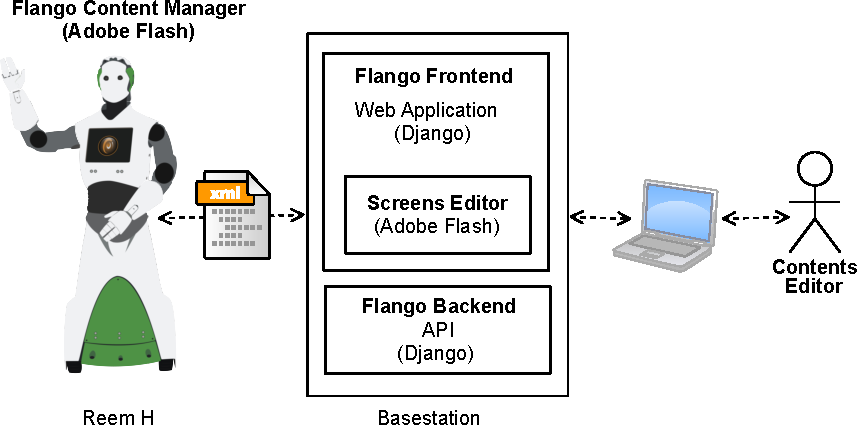
\includegraphics{figures/context-original.pdf}
    \caption{Current context}
    \label{fig:context-original}
\end{figure}

\begin{figure}[htb]
    \centering
    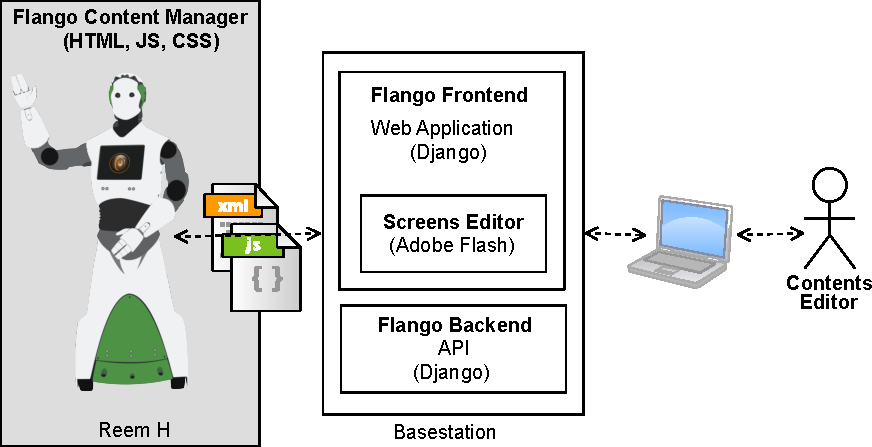
\includegraphics{figures/context-new.pdf}
    \caption{New context}
    \label{fig:context-new}
\end{figure}

\reem{H3} has about 600MB of specialised code.
The program that glues all software parts and serves as an interface to the hardware is \textbf{robotBehaviour}, developed with Qt.
A window in this program contains a QtWebKit widget, the embedded web browser that loads the contents for the touchscreen.
Contents are fetched from Basestation, a server that hosts Flango, a web application that lets users edit screens (with the \se), add media contents and synchronise them with robots (\ref{fig:context-original} on \pageref{fig:context-original}).
The \flangobe has an \ac{API} to serve the contents applications to the robots.
The project of this thesis is reengineering the Flango \cm , in the robot (\fref{fig:context-new}).

\FloatBarrier

\subsection{Interaction} 
\label{sec:interaction}
\begin{figure}[htb]
   \centering
   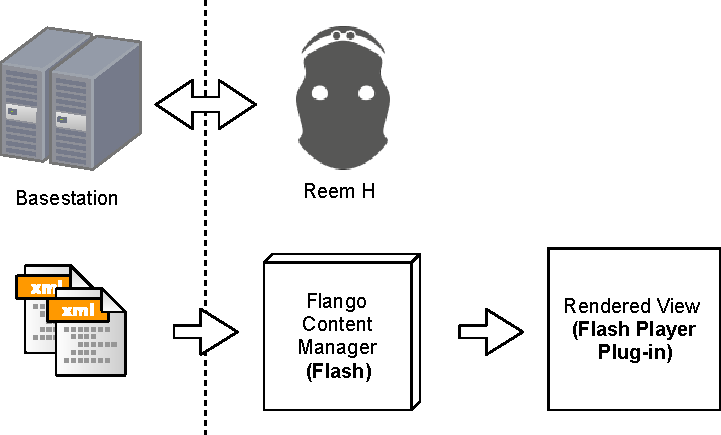
\includegraphics{figures/interaction-original.pdf}
   \caption{Current interaction}
    \label{fig:interaction-original}
\end{figure}

\begin{figure}[htb]
    \centering
    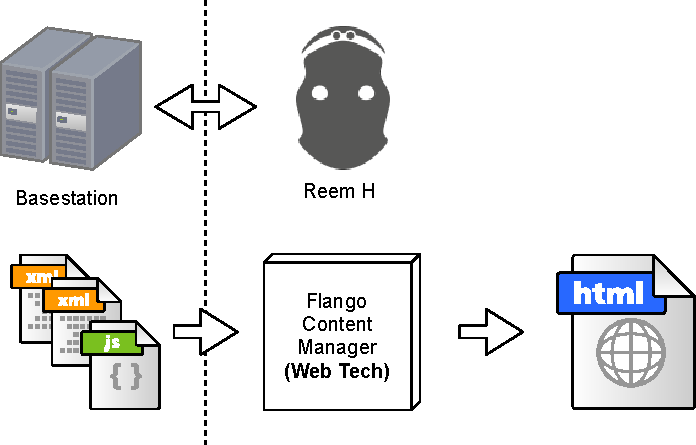
\includegraphics{figures/interaction-new.pdf}
    \caption{New interaction}
    \label{fig:interaction-new}
\end{figure}

%\begin{figure}[ht]
%    \begin{subfigure}[b]
%        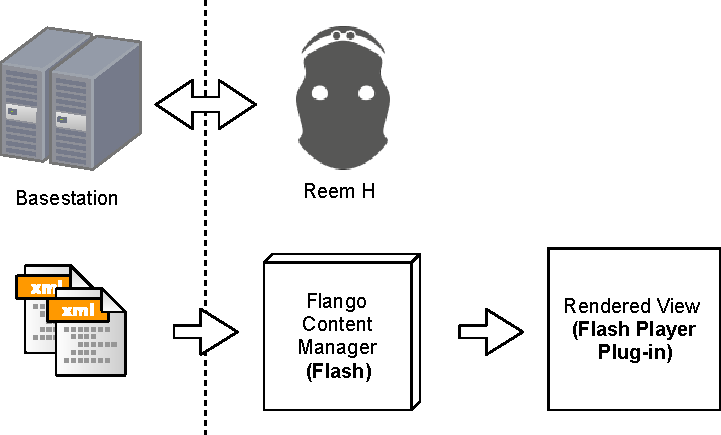
\includegraphics{figures/interaction-original.pdf}
%        \caption{Current interaction}
%        \label{subfig:interaction-original}
%    \end{subfigure}
%    
%    \hfill
%
%    \begin{subfigure}[b]
%        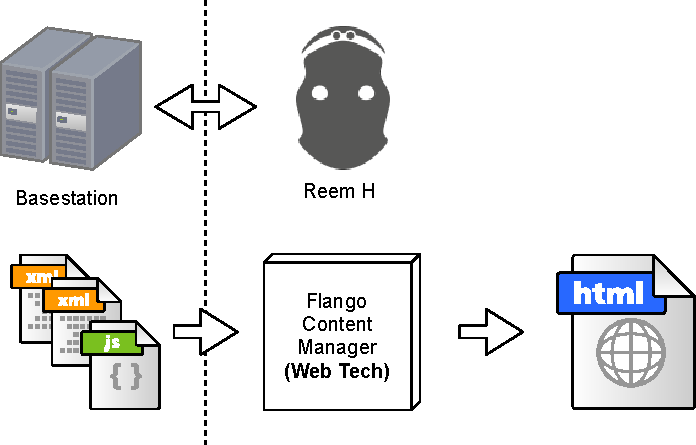
\includegraphics{figures/interaction-new.pdf}
%        \caption{New interaction}
%        \label{subfig:interaction-new}
%    \end{subfigure}
%    
%    \caption{dfgntymnrty}
%    \label{fig:smith}
%\end{figure}

The content manager's input is \ac{XML} code and the output is an \ac{HTML} single page application (\fref{fig:interaction-original} and \fref{fig:interaction-new}).
The general boot steps are:

\begin{enumerate}
    \item The robot boots
    \item robotBehaviour fetches generic settings (\ac{XML}) from Basestation
    \item The \cm uses the settings to decide which application to load, the language, the theme, etc), it requests application-specific settings and the application structure. After this, it requests the screens (the \ac{XML} files) to the \flangobe .
    \item Basestation serves all the screens
    \item The \cm renders the screens. If during this process it finds an "entity", it fetches the data from Basestation.
\end{enumerate}

\FloatBarrier

\subsection{Interoperability}
\label{sec:interoperability}
\begin{figure}[htb]
  \begin{minipage}{0.5\linewidth} 
      \centering
      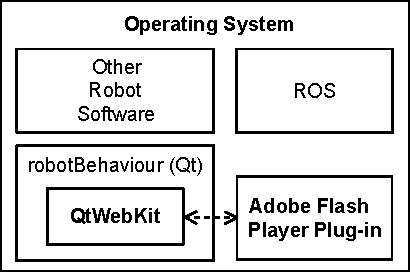
\includegraphics{figures/interoperability-original.pdf}
      \caption{Current interoperability \\ (in robot)}
      \label{fig:interoperability-original}
  \end{minipage}
  \hspace{0.5cm}
  \begin{minipage}{0.5\linewidth} 
      \centering
      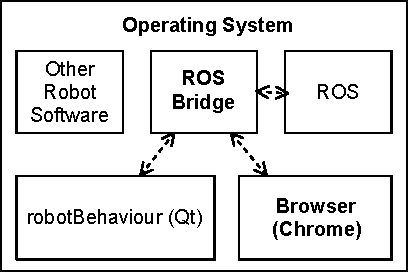
\includegraphics{figures/interoperability-new.pdf}
      \caption{New interoperability \\ (in robot)}
      \label{fig:interoperability-new}
  \end{minipage}
\end{figure}


Flango \cm interoperates with two systems: robotBehaviour and \flangobe (See figures \ref{fig:interoperability-original} and \ref{fig:interoperability-new} on \pageref{fig:interoperability-original}).

\paragraph{robotBehaviour} Flango \cm interoperates with the software of the robot through robotBehaviour, e.g. using text-to-speech capabilities or triggering a batch action (autopresentation, guide user to a certain place...).
Likewise, robotBehaviour uses an \ac{API} in Flango \cm, e.g. to restart a session or to input information gathered with the robot's hardware.
There is an interface defined for this to allow independent development in both ends.

The current system to exchange messages between the \flash container and robotBehaviour is based on JavaScript global functions.

To send a message to robotBehaviour:
\begin{enumerate}
    \item \cm (\flash) opens a new tab with a specific \ac{URL}: \texttt{flashCallback.html?\textless paramList\textgreater}
    \item robotBehaviour intercepts the call, prevents QtWebKit from opening a new tab and executes an action specified with the parameters
\end{enumerate}

To send a message from robotBehaviour:
\begin{enumerate}
    \item Calls a \ac{JS} function in the Flash website (\texttt{/static/frontend/index.html})
    \item The \ac{JS} function delegates to the Flash container
    \item The application facade of Flango Content Manager starts the required action
\end{enumerate}

The requirements state that the new software has to be implemented using web technology. 
Despite the fact that this specification should be technology agnostic, to integrate the new software better in the system, the use of \ac{ROS} Web Tools is suggested to exchange messages.
In any case, it is clear that there has to be an interface between robotBehaviour and the browser, as they run in separate processes (as opposed to sharing at least one parent process in the current implementation).

\paragraph{BaseStation (\flangobe \ac{API})} The \cm has to fetch data from Basestation in order to load the correct contents.
The \flangobe has an \ac{API} for this (\fref{tab:flango-api}):

\begin{table}[ht]
    \centering
    \begin{tabularx}{\linewidth}{| l | X |}
    \hline
    Root URL & Matching URLs \\
    \hline
    \multirow{2}{*}{\texttt{flango-api-0.1/robots}}
        & get\_robots \\ 
        & add\_robot \\
    \hline 
    
    \multirow{2}{*}{\texttt{flango-api-0.1/bl}} 
        & entity/(\textless entity\_name\textgreater).xml \\ 
        & add\_robot \\
    \hline
    
    \multirow{6}{*}{\texttt{flango-api-0.1/pal}} 
        & home \\
        & add \\
        & execute \\
        & status \\   
        & submit \\
        & history/(\textless page\textgreater) \\
    \hline
    
    \multirow{10}{2.5cm}{\texttt{flango-api-0.1/gui}  \texttt{flango-api-0.1/app}}
        & \textless app\_id\textgreater /config.\textless format\textgreater xml$|$json \\
        & \textless app\_id\textgreater /structure.\textless format\textgreater xml$|$json \\
        & \textless app\_id\textgreater /screen/(\textless screen\_id\textgreater.xml \\
        & \textless app\_id\textgreater /node/\textless node\_id\textgreater \\
        & application \\
        & node \\
        & screen \\
        & allScreens \\
        & getApps \\
        & upload\_app \\
    \hline
    
    \multirow{7}{*}{\texttt{flango-api-0.1/stats}}
        & robot/use/\textless robotID>/\textless duration\textgreater/<data\textgreater \\
        & robot/base \\
        & app/use/\textless robotID\textgreater/\textless duration\textgreater/<data\textgreater \\
        & app/top/\textless robotID\textgreater/\textless duration\textgreater/<data\textgreater \\
        & app/toptable/\textless page\textgreater \\
        & application/\textless screen\textgreater \\
        & <name> \\
    \hline
    \end{tabularx}
    \caption{Flango Backend API}
    \label{tab:flango-api}
\end{table}
Both current and new implementation use this.
However, the new implementation uses \ac{JSON} because it is more \ac{JS}-friendly: it has less overhead and it is easier to deserialise.


\section{Conceptual Model}
\begin{sidewaysfigure}[htb]   
    \centering
    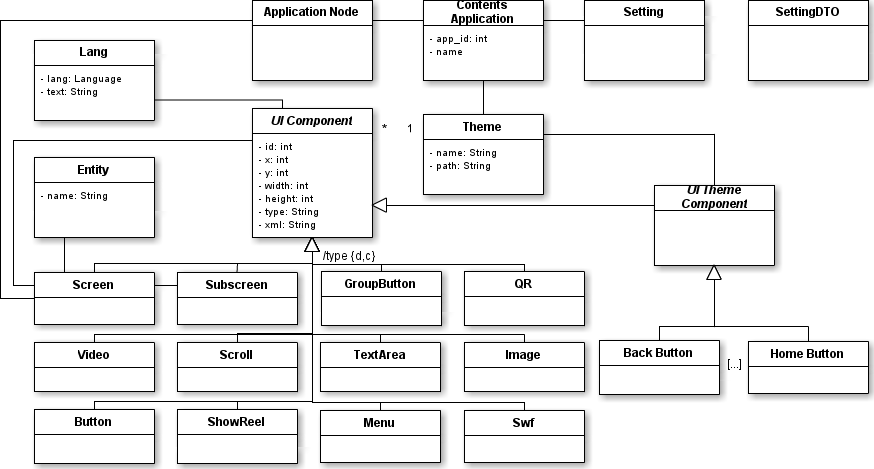
\includegraphics[width=\textwidth]{figures/specification-conceptual-model}
    \caption{Conceptual model}
    \label{fig:specification-conceptual-model}
\end{sidewaysfigure}

The new Flango \cm has to be compatible with the current implementation of the \se (\flangofe).
Otherwise, users would create contents applications with the \se that would look different when they are displayed in the robot.
To ensure compatibility, it is necessary a good understanding not only at system level, but at component level.
It is required, then, that the new implementation renders consistently all of the \ac{UI} components that the \se can create exactly like it does with the old version. 
Same applies to settings and use of "entities".

There are 7 classes: \textbf{ContentsApplication}, \textbf{ApplicationNode}, \textbf{Configuration}, \textbf{Theme}, \textbf{Screen}, \textbf{UI Components} and \textbf{Entity}.

\paragraph{ContentsApplication} A contents application with an internal identifier and a descriptive, human-friendly name.

\paragraph{ApplicationNode} An application has nodes that match the \ac{URI} with a screen.

\paragraph{Configuration} A contents application has a configuration object that can be mutated during the execution.
It represents the state of the application, the permissions, the paths to be used, etc.

\paragraph{Theme} Themes are the look and feel and default behaviour of \ac{UI} components.
The current implementation only has one (default) theme.
However, a contents application can have many themes available.
The active theme has to belong to the set of available themes. 
It encapsulates data that define it (e.g. the name, etc). FIXME etc is too short

\paragraph{Screen} A screen is the container for elements that the user can interact with.
Screens contain \ac{UI} Components and can be reused in different Application Node of the same Contents Application. FIXME: verify this

\paragraph{UI Components} A UI Component is an element of the \ac{UI}, for example a \texttt{Button} or an \texttt{Image}.
Users drag and drop them to a canvas in the Screens Editor to create the contents. 
All UI Components have an \ac{XML} code.
Because the domain of the problem and the classes are shared between the original and the new implementation, the model in \fref{fig:specification-conceptual-model} is created from the current implementation.
To support theming, there are two types of UI Components: basic (UI Component) and theme (UI Theme Component).
All UI Theme Components are eventually implemented with a basic UI Component.

\begin{lstlisting}[caption=Basic UI Components, label=uicomponents-list]
ButtonComponent.as
GroupButtonComponent.as
GroupComponent.as
ImageComponent.as
MenuComponent.as
QRComponent.as
ScreenComponent.as
ScrollComponent.as
ShowReelComponent.as
SubscreenComponent.as
SWFComponent.as
TextareaComponent.as
UIComponent.as
VideoComponent.as
\end{lstlisting}

\begin{lstlisting}[caption=Theme UI Components, label=uithemecomponents-list]
arabic_button
back_button
base_button
big_button
call_to_action_screen
camera_button
config_button
english_button
forward_button
home_button
info_button
korean_button
language_button
left_arrow_button
line
list_button
main_menu
next_button
reem_body_button
reem_button
right_arrow_button
smartphone_menu
synchronizing_screen
video_button
wide_button
\end{lstlisting}

\begin{lstlisting}[caption=Application State (Settings class), label=config-list]
api_endpoint:String
app_id:String
app_name:String
current_node:String
debug_level:String
debug_mode:Boolean
default_api_endpoint:String
def_lang:String
def_theme:String
enable_stats_bkp:Boolean
enable_stats:Boolean
history:Array
history_current:int
history_limit:int
home_node:String
initial_node:String
lang_list:Object
lang:String
log:String
media_path:String
performance_monitor:Boolean
perform_callbacks_bkp:Boolean
perform_callbacks:Boolean
redirects:Array
report_stats:Boolean
robot_id:String
scale_factor:Number
screensaver_node:String
screens:Object
screen_transitions:Boolean
security_level:int
session_fadeout:int
session_timeout:int
show_cursor:Boolean
static_api_endpoint:String
static_media_path:String
static_themes_path:String
structure:XML
theme_list:Object
themes_path:String
theme:String
themes:XMLList
zone:String

\end{lstlisting}

Listings \ref{uicomponents-list} and \ref{uithemecomponents-list} contain a comprehensive list of UI Components extracted from listing the necessary files in a package of the current implementation.
Notice that all files in \ref{uicomponents-list} have the corresponding class in the conceptual model if they have to be implemented.
The elements of \ref{uithemecomponents-list} are in fact folders but they can be considered classes in this specification as they are part of the domain of the problem.
However, some elements are not to be implemented because they are deprecated and some other components are to be implemented in future releases, but not in the software of this thesis.

\subparagraph{Excluded elements} UI Components: GroupButtonComponent, GroupComponent, ScrollComponent. UI Theme Components: call\_to\_action\_screen, main\_menu, smartphone\_menu, synchronizing\_screen.

\paragraph{Configuration} The state of the application is defined with a configuration object sent from the server.
A collection of the necessary attributes of the class that encapsulates the configuration is in \ref{uithemecomponents-list} and has been extracted from the current implementation as well.
\subparagraph{Excluded elements} Some Configuration have names tightly coupled to technology (e.g. history, history\_current, etc). 
The concept is included in the specification but not with this specific names to keep it technology agnostic.

\paragraph{Entity} Entities are classes that represent classes in the \se. 
FIXME LANGUAGE An example scenario: Alice is creating screens with the \se.
She rented the robot for a congress and wants to add information about job openings in her company.
She can define, with Flango Frontend, an entity named "Job" and use it in the screens editor to show the list of all instances of Job.
The implementation of Entities is incomplete and does not belong to the scope of this project.

\paragraph{Themes} A Contents Application can have themes.
There is a default theme that defines the look and feel and default actions on click an on load of all UI Theme Components.
All themes have the same UI Theme Components to guarantee that themes can be changed safely.
Basic UI Components look always the same way.

TODO explain XML here (NO. section ahead)? explain theming here (nothing to explain)? fallbacks ( belongs to behaviour model)? ambiguity (belongs to behaviour model r xml representation)?

Listing \fref{chap:specification-button-example-1} shows an example of the \ac{XML} definition of a Button UI Component.

\lstinputlisting[language=XML, caption={Basic UI Component Button XML}]{src/specification-button-example-1.xml}

DIAGRAM HERE

constraints?
\FloatBarrier

\section{Use Case Model}
This section describes the services of the system as sequences of events triggered by external actors.

\subsection{Actors}
The actors who use the system are:
\begin{itemize}
	\item robotBehaviour: the software that governs the \ac{GUI} of the touchscreen. It can load application contents, bring them to the front, sent them to the back, load other \ac{GUI} etc.
	\item Contents Application User: a person (or any other agent that can use a touchscreen) who interacts with the loaded contents application. Humans only interact directly with the output of this software (see \fref{sec:context}), which becomes the \ac{GUI}.
For example: the program renders a screen with one button whose action is to make Reem say "hi, my name is Reem".
The input is an \ac{XML} file, the output is a \ac{GUI} ready to be used.
Humans can now touch the button that sends events to robotBehaviour so, essentially, the \ac{GUI} of the program and not only the output is built as a function of the input.
When the \ac{GUI} is ready, a new actor (Contents Application User) and new use cases appear.
\end{itemize}


\subsection{System Use Cases}
\begin{figure}[htb]  
    \centering
    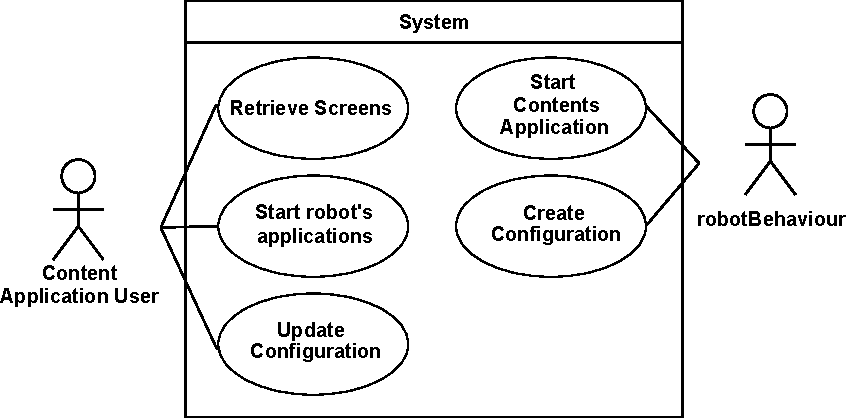
\includegraphics[width=\linewidth]{figures/specification-sucs}
    \caption{System Use Cases}
    \label{fig:specification-sucs}
\end{figure}

There is a number of use cases of the software determined by examining the current implementation at a program level.
The use cases that are implemented in this project are shown in \fref{fig:specification-sucs}.

A contents application user can see the rendered screens and update some parameters (e.g. change the language) or start applications in the robot (e.g. a Qt window with a map).
%Normally one would group use cases in "manage \ac{UC}" that include at least the \ac{CRUD} \ac{UC} FIXME plurals.
%This document does not group them because different actors
%For example: the user touches a button that makes Reem say a sentence aloud (notice that the application is sending a message to robotBehaviour).
The software system that controls the robot, robotBehaviour, can also trigger actions in the contents application (for example, it can start it).
Amongst others, it can manage the screensaver and sessions and some special settings (including: show the cursor, enable debug mode, enable start of robot's applications, contents application ID, etc). 
%Use cases Manage ScreenSaver and Manage Sessions do not belong to the scope of this project but are shown in the diagram to offer the big picture of the Flango Content Manager.

\begin{suc}
{title of the use case}
{a description}
{actors}
{preconditions}
{postconditions}
{main scenario
    \begin{enumerate}
        \item first step
        \item second step
    \end{enumerate}
}
{extensions}
\end{suc}

\begin{suc}
{Start Robot's Applications}
{A user can start robot's applications like face recognition, ball grasping, meet people, etc.}
{Content Application User}
{robotBehaviour is running}
{The chosen robot application starts}
{
    \begin{enumerate}
        \item The User chooses a robot's application and asks the system to start it
        \item The system starts the application
    \end{enumerate}
}
{None}
\end{suc}

\begin{suc}
{Start contents application}
{robotBehaviour wants to display the application on the touchscreen of the robot}
{robotBehaviour}
{
	\begin{enumerate}
        \item robotBehaviour is running
        \item The application has been synchronised with the robot (i.e. the robot has all the necessary parts to load it)
    \end{enumerate}
}
{
The initial screen of the contents application is shown
}
{
    \begin{enumerate}
        \item robotBehaviour determines the $app_id$ and asks the system to load the application with the given $app_id$ and initialisation parameters.
        \item include Manage Configuration
		\item the system loads the initial screen
    \end{enumerate}
}
{    
	\begin{itemize}
        \item The application can't be found
        \begin{enumerate}
        	\item The system shows a default screen
    	\end{enumerate}
    	\item The application contains errors
        \begin{enumerate}
        	\item The system degrades progressively the contents application
    	\end{enumerate}
    \end{itemize}    
}
\end{suc}


\begin{suc}
{Manage Configuration -- Create}
{The system fetches the configuration (on load) from the Backend. If it can't be found, it falls back to a default configuration. FIXME: no clear actor}
{Event on-load}
{
	\begin{enumerate}
        \item robotBehaviour is running
        \item The application has been synchronised with the robot
    \end{enumerate}}
{
The configuration object is created
}
{
    \begin{enumerate}
        \item robotBehaviour starts the Flango Content Manager
        \item The system requests the generic configuration to the Backend
		\item The Backend sends the generic configuration $c$
		\item The system requests the application-specific configuration for application $c.app_id$ or $auto$
		\item The Backend returns the application-specific configuration $sc$
		\item The system requests the application structure
		\item The Backend returns the application structure $as$
		\item The system reads the URL query string that overwrites parameters
		\item The system creates the configuration object
    \end{enumerate}
}
{    
	\begin{itemize}
        \item The generic configuration can't be found
        \begin{enumerate}
        	\item The system displays an error message
    	\end{enumerate}
    	\item The application specific configuration can't be found
        \begin{enumerate}
        	\item The system loads the default application and displays an error message
    	\end{enumerate}
    	\item The application structure can't be found
        \begin{enumerate}
        	\item The system displays an error message
    	\end{enumerate}
    \end{itemize}   
}
\end{suc}

\begin{suc}
{Manage Configuration -- Update}
{The contents application user changes a parameter in the configuration or an event related to update the configuration is received}
{Contents Application User, events}
{
	\begin{enumerate}
        \item robotBehaviour is running
        \item The application has been synchronised with the robot
        \item The configuration object is initalized
    \end{enumerate}
}
{
The configuration object is mutated
}
{
    \begin{enumerate}
        \item The user asks the system to retrieve the configuration object
        \item The system returns the configuration object
        \item The user changes a value and asks the system to store it (e.g. current language)
		\item The system updates the configuration object (FIXME and notifies the system?)
    \end{enumerate}
}
{     
}
\end{suc}

FIXME note: delete and retrieve are not exposed to the user. just for internal use.



\begin{suc}
{Retrieve Screen}
{The content application user navigates to a screen }
{Contents Application User}
{
	\begin{enumerate}
        \item robotBehaviour is running
        \item The application has been synchronised with the robot
        \item The application is loaded
    \end{enumerate}
}
{
The requested screen is shown
}
{
    \begin{enumerate}
		\item The user asks the system a list of screens (e.g. a screen with buttons)
        \item The system offers a list of screens to go
        \item The user chooses a destination
        \item The system shows the requested screen
    \end{enumerate}
}
{
    \begin{itemize}
	    \item The screen is unavailable
	    \begin{enumerate}
	    	\item The system shows an error
	    \end{enumerate}
    \end{itemize}
		
}
\end{suc}

\FloatBarrier

\section{Behaviour Model}
This thesis combines \ac{DbC} and \ac{TDD}, two techniques that are not mutually exclusive.
Basically, tests define the behaviour for specific cases and \ac{DbC} defines the general behaviour. 
Thus, there are no tests for edge cases or negative behaviours because contracts, and more specifically preconditions, protect the component.
In spite of the name, \ac{TDD} tests are executable specifications.
They become tests only after having implemented all the functionality being test-driven.
Before this, there is nothing to actually test and these artifacts are rather executable specifications, but not tests.
Tests (specifications) are written before the code and define the behaviour of components.

Additionally, they are used as documentation of the software but they are not sufficient to completely define the behaviour because they only assert properties by example instead of stating general properties (e.g. "it should return 5" vs "return value $1 \leq x \leq 10$"). The latter can be achieved using formal specifications, e.g. using Meyer's \ac{DbC} \cite{Baumeister:2004}.

In this thesis, tests are implemented with Jasmine and AngularJS but this chapter focuses on what the tests describe rather than how they are executed and controlled.

Combining the two techniques one can use the best parts of each to define the behaviour of the system.
With \ac{TDD}:
\begin{itemize}
    \item Build only what is required (Keep it simple and control the scope of the project)
    \item Drive design decisions from tests (i.e. from the specification)
\end{itemize}

\noindent With formal specifications (\ac{DbC}):
\begin{itemize}
    \item Higher code quality
    \item Less checks (preconditions)
    \item Drive design decisions from preconditions
\end{itemize}


%Larman: system sequence diagram + Meyer: contracts of system operations
%"System Sequence Diagrams:
%–
%Identify system events and system operations
%–
%Identify system events and system operations
%– Document sequence of interactions
%• Contracts:
%– Define the pre- and post-conditions for system
%operations "

%up to date documentation: a common problem is that docs are hardly ever updated

Contracts of operations define system behaviour and describe the outcome of executing system operations in terms of state changes to domain objects.
This section contains the sequence diagrams and contracts of the most relevant operations in the system.
However, the most complex part of this project is parsing and rendering the input \ac{XML} files.
Users do not interact directly with them: they do not execute operations that result in state changes to the domain object.
\fref{chap:design} explains this problem and the solution in detail.

\subsection{Sequence diagrams}
\begin{figure}[htb]
    \centering
    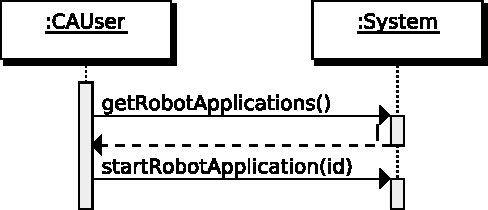
\includegraphics{figures/spec-seq-start-qtapp.pdf}
    \caption{System Sequence Diagram - Start Robot Applications}
    \label{fig:spec-start-qtapp}
\end{figure}

\begin{figure}[htb]
    \centering
    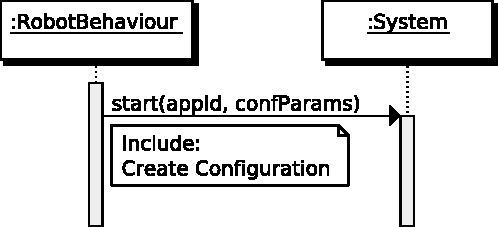
\includegraphics{figures/spec-seq-start-contents-app.pdf}
    \caption{System Sequence Diagram - Start Contents Applications}
    \label{fig:spec-start-ca}
\end{figure}

\begin{figure}[htb]
    \centering
    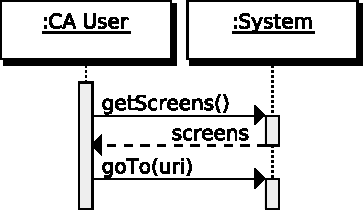
\includegraphics{figures/spec-seq-manage-screens-read.pdf}
    \caption{System Sequence Diagram - Manage Screens (Read)}
    \label{fig:spec-manage-screens-read}
\end{figure}

\begin{figure}[htb]
    \centering
    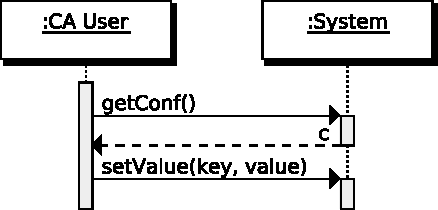
\includegraphics{figures/spec-seq-manage-conf-update.pdf}
    \caption{System Sequence Diagram - Manage Configuration (Update)}
    \label{fig:spec-manage-conf-create}
\end{figure}

\begin{figure}[htb]
    \centering
    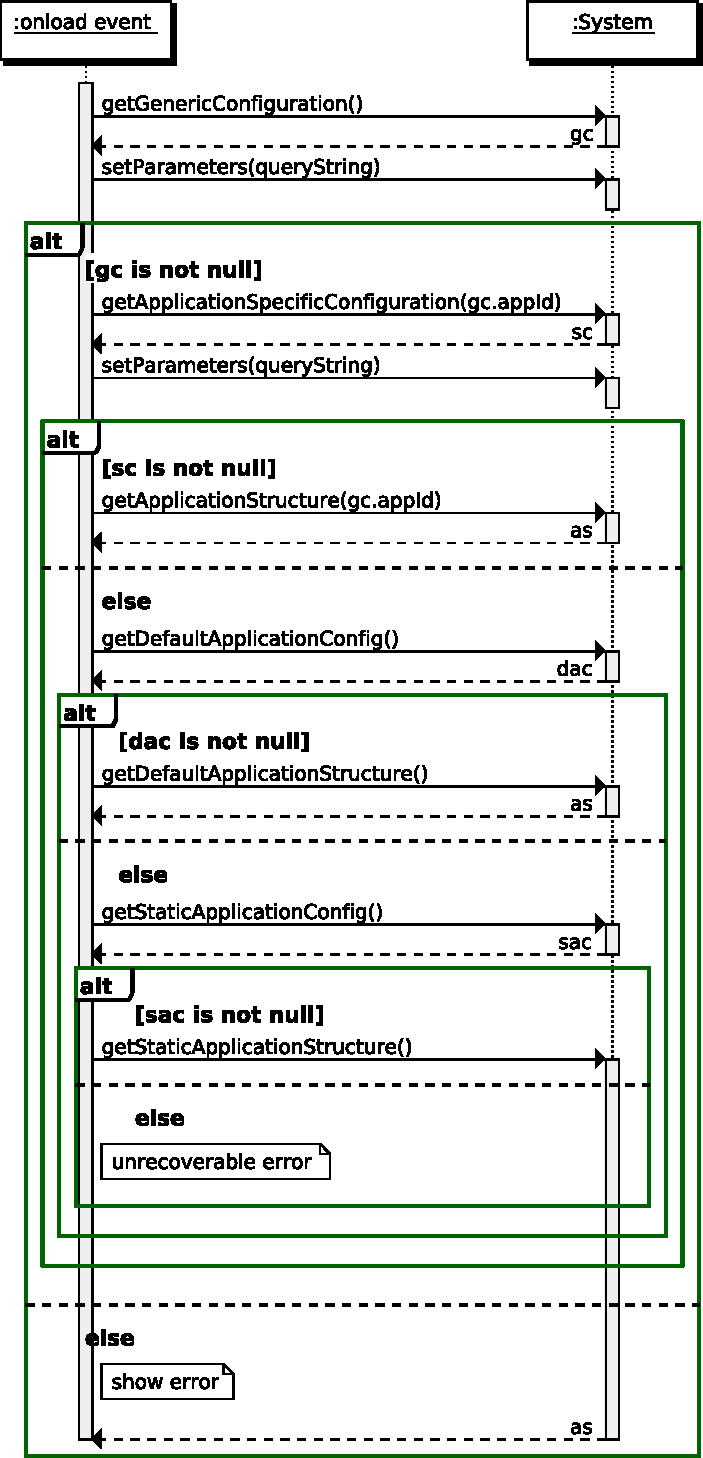
\includegraphics{figures/spec-seq-manage-conf-create.pdf}
    \caption{System Sequence Diagram - Manage Configuration (Create)}
    \label{fig:spec-manage-conf-create}
\end{figure}

\subsection{Contracts}
system operations

\begin{sopcontract}{nameofopaaa}
{description}
{preconditions go here}
{postconditions go here}
\end{sopcontract}

FIXME: robot behaviour ja no cal!!

\begin{sopcontract}{getRobotApplications()}
{FIXME: this is part of the contents of an XML file, like functions.xml. Maybe it should not be here. Retrieves a list of applications that can be launched from the Flango \cm , e.g. Qt applications like navigation or face recognition.}
{RobotBehaviour is running}
{A list \texttt{l} of robot applications was returned}
\end{sopcontract}

\begin{sopcontract}{startRobotApplication(id:String)}
{Starts the robot application with id \texttt{id}, e.g. 'face recognition'}
{\texttt{id} is a valid robot application identifier}
{A request to start the robot application with id \texttt{id} was sent}
\end{sopcontract}

\begin{sopcontract}{start(appId: Integer, confParams: HashMap)}
{Starts the contents  application with id \texttt{appId} and configuration parameters \texttt{confParam} that can overwrite the fetched configuration from the backend}
{\texttt{id} is a well-formatted contents application identifier}
{FIXME aaaa}
\end{sopcontract}

\begin{sopcontract}{getScreens(appId: Integer)}
{Obtains the screens of the contents application with id = \texttt{appId}}
{\texttt{id} is a well-formatted contents application identifier}
{A list of all screens of application contents with id = \texttt{appId} was returned}
\end{sopcontract}

\begin{sopcontract}{goTo(appId: Integer, uri: String)}
{Displays the desired screen}
{
\begin{enumerate}
    \item \texttt{id} is a well-formatted contents application identifier 
    \item \texttt{uri} is a well-formatted screen \ac{URI} in the contents application
\end{enumerate}
}
{\texttt{Conf.currentScreen} was set to \texttt{uri}}
\end{sopcontract}

\begin{sopcontract}{getConf(appId: Integer)}
{Obtains the local configuration object for the application \texttt{appId}. This object is stable during the execution of the program. It does not need to be fetched again from the Backend.}
{\texttt{id} is a well-formatted contents application identifier}
{The configuration \texttt{c} was returned}
\end{sopcontract}

\begin{sopcontract}{setValue(c: Conf, key, value)}
{Sets a field of the configuration object to the desired value.\\ e.g. \lstinline$setValue(c, 'currentLang', 'de')$}
{
\begin{enumerate}
    \item \texttt{key} is a valid field of the configuration object \texttt{c}
    \item \texttt{value} is a valid value for \lstinline$c[key]$
\end{enumerate}
}
{\lstinline$c[key]$ was set to \texttt{value}}
\end{sopcontract}

\subsection{Unit Tests}
FIXME NOTE: high level description of the tests. specification by example

\fref{fig:specification-conceptual-model} describes the real world and shows the relationship between elements that define the problem.
Actors do not interact with most of the classes shown and contracts and sequence diagrams are intented to describe the system as a unit that provides some service to actors.
One of the goals of this project is making it compatible with the current \ac{XML} that defines the contents applications.
To meet this goal, it should be clearly specified how \ac{XML} are parsed.
This project uses \ac{TDD} and has executable specifications for all parts of the system, including those (e.g. internal operations or parsing) that are not strictly eligible for other sections in this chapter.

Tests are organised in test-suites for components and each suite has several test cases.
This section focuses on the \ac{XML} description.

\Fref{chap:testing} has a full list and examples of other test suites that refer directly to components of the software (described in \fref{chap:design})
Tests challenge behaviour like reading text nodes in \ac{XML} tags, setting properties (i.e. mutating correctly an object in the system), reading order or inheritance of properties, fallback to default values and transformation to \ac{HTML} code.

An example of specifications by example:

Unit testing UI directive
\begin{enumerate}
	\item inline type property: should have type defined
	\item width, height, x, y, 
		\begin{enumerate}
			\item should have the class hide
			\item should set the property to 42 for the default (language-independent)
			\item should set the property to 40 for Catalan and 42 for French
			\item should set the property to 40 for Catalan, 42 for French and 20 for default
			\item should not set any property
			\item (inline) should set the property to 42 for the default (language-independent)
			\item should set the property to 42 for default (language-independent) of pal-container
			\item (inline) should set the property to 42 for default (language-independent) of pal-container 
		\end{enumerate}
\end{enumerate}

\textbf{A comprehensive list is available in \fref{chap:app-unittests}}.


\section{XML Representation}
explain syntax here?

at least the inheritance and themes. with code.
 % spec
\chapter{Design}
\label{chap:design}
This chapter describes the internal wiring of the application and the reasons that lead to this design.
It explains the programming languages, frameworks and most relevant libraries, 

\section{Overview}
Reverse engineering the current project involves 3 activities related to technology and implementation details: \textbf{code restructuring}, \textbf{data restructuring} and\textbf{ forward engineering}.
No modifications in the code of the old version of Flango \cm are scheduled: there is no code or data restructuring.
However, there are some adaptations to be done in the \flangobe (\ac{API}), \ac{XML} and robotBehaviour:

\paragraph{Changes in \flangobe} The \ac{API} is designed to return \ac{XML} in all cases.
Most of the time this is desirable (e.g. requests to get screens) but in cases where normal exchange of information is done between the two systems, \ac{JSON} is a better option for the new technology.
It is less verbose (minimise bandwidth) and has a straight-forward translation to JavaScript objects.

\paragraph{Changes in \ac{XML}} The \ac{XML} syntax is designed to work isolated.
The new version, however, can mix \ac{XML} with \ac{HTML} thanks to Angular.
This leads to two problems:
\begin{itemize}
\item Some tags of the \ac{XML} vocabulary conflict with \ac{HTML}. For instance, \texttt{caption}. Solution: add a namespace \texttt{fl} to all tags. Thus, in the new version a \\ \lstinline$<ui type="base-button"></ui>$  becomes\\ \lstinline$<fl:ui fl:type="base-button"></fl:ui>$ .
\end{itemize}

\paragraph{Changes in robotBehaviour} Current interoperation between Flango \cm and the robot is limited to robotBehaviour.
This communication is done with JavaScript callbacks and \acp{URL}.
To decouple the \cm as much as possible from the rest of the robot, the new system uses \ac{ROS} Topics and ROS Bridge

\subsection{Forward Engineering} A program that depends on a dead browser plug-in with performance issues is not sustainable.
A solution is completely  redesigning, recoding and retesting the program, even with a different technology that makes it more flexible, open to new developers and without performance problems.


\section{Technology}
angularJS (teach the browser new syntax), javascript, html5, Qt, QtBrowser and its limitations (JS engine vs chrome v8 or firefox's). tdd+jasmine

The project of this thesis, Flango \cm, is designed to work client side in a web browser.
The natural technology in this environment is JavaScript, HTML and CSS.
It uses the Google AngularJS framework with jQuery.
Angular \textit{teaches the browser new syntax}.
That is, instead of parsing the \ac{DOM} tree and building the \ac{GUI}, it defines the behaviour of new tags in \ac{HTML} documents that can be treated as regular \ac{HTML} nodes in the \ac{DOM}.
It interoperates with other systems built with a different technology: components in the robot use \ac{ROS} and the \flangobe has an \ac{API} (see sections \ref{sec:context}, \ref{sec:interaction} and \ref{sec:interoperability} on page \pageref{sec:context}).

\subsection{JavaScript}
THIS SUBSECTION  IS NOT WRITTEN.

some hints. functional. scopes.
language, jquery, qr, swf

Object Literal Notation, constructors, closures, var scope, concept of classes
notes:

First thing you need to know is that JavaScript uses prototype-based inheritance. This means there is no distinction between classes and instances as in other OO languages (like Java). There are just objects. One implication of that is that differentiating between class and object diagrams does not make sense.

Keep in mind that UML includes many types of diagrams, specifically a branch of behavior diagrams, including sequence and use case diagrams. Such diagrams specifically address your concern of modeling javascript as a behavior driven language.

It is quite possible that a javascript system is not using object-oriented design. In such a case, class diagrams would probably not be appropriate, as you pointed out. However, since javascript does support object-oriented design, it is possible for class diagrams to effectively depict a system using javascript. It really depends on how the javascript is being used.

JavaScript is an
object-based
language. Just as in C\#, you can create objects, call their
methods, pass them as parameters, and so on. You could see this clearly when working
with the DOM, where you manipulated the HTML document through the methods
and properties of the implicit
document
object. However, JavaScript isn't generally
considered a fully object-oriented language because it lacks support for some features
that you'd
fi
nd in "real" OOP languages, or simply implements them differently.

 What does "object-oriented programming" mean anyway? Basically, as the name
suggests, OOP puts objects at the centre of the programming model. The
object
is
probably the most important concept in the world of OOP—a self-contained entity
that has
state
and
behavior
, just like a real-world object. Each object is an instance of a
class
(also called
type
), which de
fi
nes the behavior that is shared by all its objects


******

description of the language and big uses
objects
functions
prototypal inheritance (vs classical model, new, etc)


\subsection{AngularJS}
The framework enforces a very strict separation of responsibilities: \ac{DOM} updates are abstracted away from model updates. 
Directives act as the layer that keeps the two parts loosely coupled.
On one hand, directives translate data into user interfaces and, on the other hand, directives translate user interactions back into \texttt{\$scope} behaviors. FIXME Reword this

\paragraph{Overview} AngularJS is a framework for dynamic web applications.
\ac{HTML} was created to declare static documents and needs libraries and frameworks to enable application development.
Angular lets developers use \ac{HTML} in the templates and extend the language syntax to express reusable components.
It \textit{teaches the browser new syntax} through a construct called Directive.
Features:
\begin{itemize}
    \item Tools to build \ac{CRUD} Applications: data-binding, basic templating directives, form validation, routing, deep-linking, reusable components, dependency injection.
    \item Tools to test: unit-testing, end-to-end testing, mocks.
\end{itemize}

Flango \cm reads \ac{XML} and renders it as \ac{HTML}.
There are two possible approaches: parsing the \ac{DOM} tree in the browser or teaching the browser new syntax.
This project uses the second (FIXME language: the latter?): instead of developing an algorithm to traverse the tree and render elements, it defines reusable components (AngularJS Directives) and includes the \ac{XML} files in the appropriate place in the \ac{DOM}. 
The browser already traverses the tree to render the page and there is no need to do it manually.
Normally a browser ignores an element that doesn't belong to the \ac{HTML} specification (e.g. \lstinline$<fl:ui fl:type="base-button"></fl:ui>$)
With AngularJS, the browser runs the behaviour defined in the reusable component.

\paragraph{Building Blocks} There are several key components in AngularJS to build the application.

\begin{itemize}
    \item \textbf{Controller}: a function that binds the view with the model. It typically assigns objects to the \$scope variable to expose them to the template.
    \item \textbf{Directive}: a construct to extend HTML with custom attributes and elements. It defines the template of the reusable component, the behaviour, the attributes, etc. For instance, the directive \texttt{flBaseButton} states that the node \lstinline$<fl:ui fl:type="base-button">$ in the \ac{DOM} tree should be transformed into a simple \texttt{button} using the theme template \texttt{baseButton.xml}. 
    \item \textbf{Service}: Singleton that encapsulates reusable business logic independent of views. For instance, a service to handle the configuration of the application. They can be injected in controllers, directives or other services.
    \item \textbf{Filter}: a function that formats the value of an expression for display to the user. For instance, a filter to display a Number with currency format.
    \item \textbf{Module}: These building blocks are grouped in Modules. They can have dependencies between them.
\end{itemize}

The framework provides all the necessary tools to use unit and end-to-end testing from the very beginning of the project.
Considering testing as equal in importance to application writing makes the code to be more robust, lowers the cost of maintenance and helps to have a better internal design.
\begin{itemize}
    \item \textbf{Jasmine} is a behaviour-driven development framework for testing JavaScript code. It does not depend on any other framework and does not require a \ac{DOM}. It provides a simple, self-descriptive (FIXME language!) syntax to write test suites.
    \item \textbf{Angular Mocks}: there are stub objects ready to load in tests (e.g. \texttt{\$httpBackend} mocks \ac{HTTP} calls)
    \item \textbf{Karma} is a test runner to automate the execution of the test suites. 
\end{itemize}
    
\paragraph{Compile-Link} To make directives possible Angular has a compiler.
In this context, compiling means attaching event listeners to the \ac{HTML} to make it interactive.
The compiler traverses the \ac{DOM} tree in two phases:
Firstly it looks for tags that have directives associated (e.g. \lstinline$<fl:ui fl:type="base-button">$ or even native \ac{HTML} elements \lstinline$<a>$).
Secondly it binds the model to the view.
The compiler allows developers to attach behaviour to any \ac{HTML} element or attribute and even create new HTML elements or attributes with custom behaviour.
Angular calls these behaviour extensions directives.

The order of execution is:

\lstinputlisting[language=xml, caption={Order of execution of directives}]{src/example-order-directives.xml}

\lstinputlisting[language=bash, caption={Result of execution of directives}]{src/result-order-directives.text}

The role of these functions is:
\begin{itemize}
\item \textbf{Directive Controller}: similar to regular controllers but accessible from other directives. 
\item \textbf{Compile}: finds new directives and runs their compile function. Modifications to the \ac{DOM} before applying the template can be done here.
\item \textbf{Link}: binds data to the view. Modifications to the final \ac{DOM} are safe to do here.
\end{itemize}

\paragraph{Directive} At a high level, directives are markers on a \ac{DOM} element (such as an attribute, element name, \ac{CSS} class or a comment) that tell Angular's \ac{HTML} compiler to attach a specified behaviour to it or even replace it with another element.
The \ac{HTML} compiler finds elements that match directives. 
For example, for \lstinline$<div ng-controller="myCtrl">$, the element \texttt{div} matches the directive \texttt{ngController}.
An example in Flango Content Manager: when the browser finds \lstinline$<fl:width>150</fl:width>$ in the \ac{DOM}, the element \texttt{width} matches the directive \texttt{flWidth}.
The \texttt{flWidth} directive is restricted to elements (it matches \lstinline$<fl:width>150</fl:width>$ but not \lstinline$<div fl:width>150</div>$ because it is an attribute), and it has a custom \texttt{link} function that performs some computation.

    
\subsection{HTML5}
maybe not useful. maybe just html

\subsection{SASS}
Writing plain \ac{CSS} can be tedious and error-prone.
SASS stands for Syntactically Awesome CSS and is a pre-processor with syntax advancements that add features to \ac{CSS}.
Sass is an extension of \ac{CSS}3, adding nested rules, variables, mixins, selector inheritance, and more.
It is then translated into well-formated, standard \ac{CSS} using the command line tool.
This makes reusing and extending \ac{CSS} easier.
SASS has two syntaxes. This project uses the newest one, known as \ac{SCSS} (Sassy CSS).

A key feature in this project is the \lstinline$@extend$ directive: it tells \ac{SASS} that one selector should inherit styles of another selector.
Example: the style \texttt{base-button} has a grey background. The style \texttt{button} sets the size of the element to $100 x 50 px$.
Because all \texttt{base-button}s are \texttt{button}s, the first should inherit the style from the second instead of replicating it, like one would do with \ac{OOD}.
With \ac{HTML} this would be written \lstinline$<div class="base-button button" />$.
With SASS one can write \lstinline$.base-button { @extend .button }$ and keep \ac{HTML} cleaner: \lstinline$<div class="base-button" />$

SASS variables and mixins make it easier to scaffold (FIXME LANGUAGE!) themes for Flango Content Manager and have consistency in the visual design (e.g. all themes can have palettes of the same size).

\subsection{Robot Web Tools}
Robot Web Tools is a collection of open-source modules and tools for building web-based robot applications.
It provides 3 core libraries to communicate with \ac{ROS} on the robot over rosbridge's WebSocket server: roslibjs, ros2js, and ros3djs.
This project uses roslibjs to subscribe and publish to Topics.

\section{Architecture}
context: comm with rob behaviour and rostopics (SOA).
MVC. client-side. JSON to talk to an API. xml files as angularjs partials, hacks to make it work (routes defined manually, one controller for all of them, dirty entities). scopes and their specific use here (compare to regular use). what about MVVM?

common patterns:
dependency injection and angularJS (and literature: fowler)

\subsection{Robot Operating System}
Flango \cm is a piece in the robot.
\ac{ROS} is a framework for robot software development that provides operating system-like functionality on a heterogeneous computer cluster. 
It was originally developed in 2007 as part of the Stanford AI Robot (STAIR) project with the goal of providing an architectural framework supporting modular, tool-based development for robotic software.
It has a loosely coupled architecture with nodes, messages, topics and services, similar to \ac{SOA} \cite{ROS:2008}.

Nodes are processes that perform computation, a "software module". 
Nodes communicate with each other by publishing/subscribing with two protocols:
\begin{itemize}
\item Topics: asynchronous. message passing (publish/subscribe). Typed by a \ac{ROS} Message
\item Services: synchronous. \ac{RPC} (pairs of request/response messages). Typed by a \ac{ROS} Service
\end{itemize}

Messages are strictly typed data structures . There are some available by default, like \texttt{std\_msgs/String} and other primitive types.
To find service in this peer-to-peer topology, there is a lookup mecanism: \emph{rosmaster} \fref{fig:design-ros-topics} and \fref{fig:design-ros-services}.

The robot has two parts: robotBehaviour and Stacks.
Part of the code of the robot (robotBehaviour) does not follow the \ac{ROS} workflow but still uses Topics to communicate with the Stacks, the part of the project that does use \ac{ROS}.
In Stacks there are Servers and ActionServers that provide Services.
Flango \cm is a component in this system that communicates with robotBehaviour using \ac{ROS} Topics and two types of messages.
It is not designed strictly as a service to handle synchronous requests but it is able to use Topics to have asynchronous requests and provide feedback, like ActionServers.
A typical use of a \ac{ROS} Topic is setting the language of the \cm or sending an action to robotBehaviour (e.g. shake hands, say a sentence).
robotBehaviour is not a \ac{ROS} service and therefore it can not handle request/responses like other components in the system.
Topics are the only way to communicate with it.

\begin{figure}[htb]
    \centering
    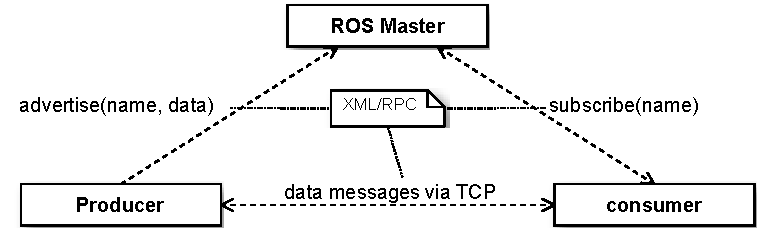
\includegraphics{figures/design/ros-architecture-topics.pdf}
    \caption{High-level view of the ROS Architecture (Topics)}
    \label{fig:design-ros-topics}
\end{figure}

\begin{figure}[htb]
    \centering
    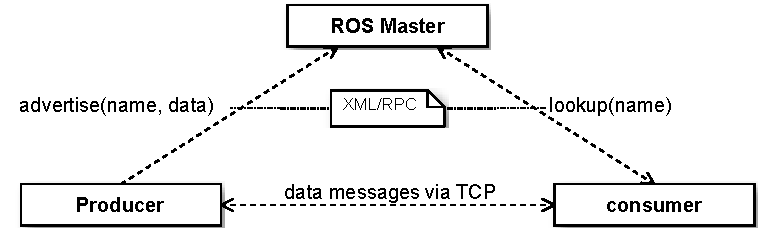
\includegraphics{figures/design/ros-architecture-services.pdf}
    \caption{High-level view of the ROS Architecture (Services)}
    \label{fig:design-ros-services}
\end{figure}

FIXME diagrams ROS-flango-robot-robotbehaviour etc go here? in specs  just include the description of what the system does.

ROS i SOA.
robotbehaviour
flango as a (bad) service.



\subsection{MVC}
\ac{MVC} is a decoupled architecture with a strong separation of responsibilities (\fref{fig:mvc-overview}).
\begin{itemize}
    \item \textbf{Model} (application state). Maintains application state and notifies dependent views and controllers when changes occur (with the observer pattern)
    \item \textbf{View} (output) queries the model to print [parts of] it, listens for changes in the model
    \item \textbf{Controller} (input) Listens for input and tells the model or the view to change accordingly
\end{itemize}

It is possible to have multiple views and controllers for the same model and they can be reused for other models.

Angular applications take the most of the framework when they are designed with a \ac{MVC} architecture.
A typical use case in a \ac{MVC} application might be:
\begin{itemize}
    \item Model: [orange, apple, pineapple, coconut]
    \item View: displays a list of 2 random pieces of fruit
    \item Controller: logic that decides to fetch two pieces of fruit
\end{itemize}

Flango \cm does not have a \ac{GUI} or a set of predefined and stable use cases.
This changes for every contents application.
The system only knows the use cases after loading the contents application.
There can not be controllers for application-specific use cases and the view is created dynamically from the model.

\begin{itemize}
    \item \textbf{Model}: screens definitions, entities, configuration... stored in the backend
    \item \textbf{View}: built dynamically from the model. The application loads screens as the user browses to \ac{URL}s and transforms them to \ac{HTML} so that they can be displayed in the browser.
    \item \textbf{Controller}: Typically, controllers in Angular manage the \texttt{\$scope} and expose behaviour to the View. This application has some generic (as opposed to application-specific) ones. For example: an instance of \texttt{ActionCtrl} for each button, a \texttt{ROSBridgeCtrl} to respond to requests from ROS Bridge, etc. Directives also have a special type of controllers: Directive Controllers are defined within the context of one directive but they can be injected into other directives to facilitate inter-directive communication. For example, a controller in the \texttt{flUi} directive manages its properties (\texttt{x}, \texttt{y}, \texttt{width}, \texttt{height}, \texttt{caption}...). \texttt{flWidth}, \texttt{flX}, and other directives use the controller in \texttt{flUi}.
\end{itemize}

Angular uses an \ac{MVC} pattern with two-way data binding \fref{fig:mvc-with-observer}: changes in the view are reflected to the model immediately and viceversa in order to use the model as a single source of truth.
Controllers use the \texttt{\$scope} to expose values and behaviour to the view: they update the object that is used in the view.
The \texttt{scope} is an object that refers to the application model.
Informally, it is the glue between the controller and the view.
FIXME: SURE? Controllers are completely separated from the view and unaware of it: they just expose values but do not manipulate the \ac{DOM} or read it in any way to make testing easier.

\begin{figure}[htb]
    \centering
    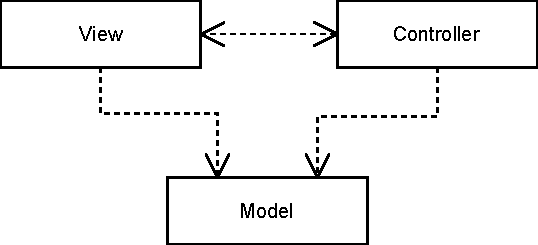
\includegraphics{figures/design-patterns-mvc-1.pdf}
    \caption{MVC overview}
    \label{fig:mvc-overview}
\end{figure}

\begin{figure}[htb]
    \centering
    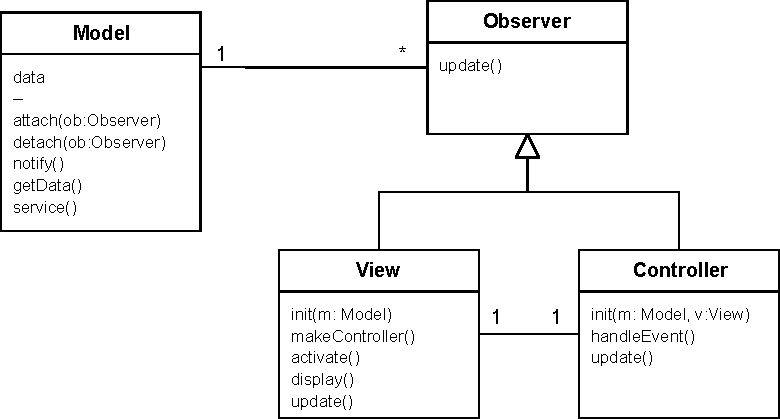
\includegraphics{figures/design-patterns-mvc-2.pdf}
    \caption{MVC with observer pattern}
    \label{fig:mvc-with-observer}
\end{figure}

\subsection{Common Patterns in the project}
DI, inversion of dependency, reveal, factory, async, fowler... hints of the remote façade and SOA¿?

This subsection is a high-level description of the most relevant software patterns in the project.

\paragraph{Constraints}
FIXME this section sucks 
%Flango Content Manager has  been designed taking into account the guidelines of \ac{GRASP} and the five basic principles of \ac{SOLID}.
The project follows object-oriented design adapted to the constraints induced by the technology and the requirements of the project.

FIXME improve this:
\begin{itemize}
    \item The \textbf{Angular Framework} is an approach to Web Components but components are not fully reusable. Moreover, most of the cl
    \item  Legacy \ac{XML}. The contents application uses \ac{XML} to define screens, templates, components, etc. The vocabulary and grammar of this \ac{XML} was designed having Adobe Flash and imperative programming in mind. While imperative programming is great for business logic, Angular prefers declarative programming for the view. 
%    \item This project is not a traditional \ac{CRUD} application. The model is a set of screens and 
\end{itemize}

 FIXME these are horrible paragraphs:
\paragraph{\ac{GRASP}} The patterns used in \ac{GRASP} are: Controller, Creator, Indirection, Information Expert, High Cohesion, Low Coupling, Polymorphism, Protected Variations, and Pure Fabrication. 
Angular enforces a strict separation of concerns between components and together with \ac{TDD} and unit testing, it helps keeping components loosely coupled.
The framework provides an easy way to create Controllers, non-user interface objects responsible for receiving and handling events.
They are mediators between the model and the view (indirection pattern). 
For example, $ActionCtrl$ for buttons receive events from the \ac{UI} and delegate the action to the corresponding class.
New elements of the framework, like Services or Directives, are created using a factory function.
FIXME However, the model are the screens and instead of creating an object from an \ac{XML} file the system just appends it to the \ac{DOM} and defines the behaviour in Directives, the software hardly ever has to create instances of objects explicitly.
FIXME should this be here?: The model is stable during the execution of the application. That is, new instances of classes of the model can not be created. 
New instances of classes are hardly ever created because the model is stable during the execution of the application. 
Changes are not made persistent. 
The application retrieves the model, renders it and lets the user interact with the contents in the touchscreen.

\paragraph{\ac{SOLID}} Five basic principles in software design are present in this project.
Classes have a single responsibility (e.g. Configuration for the \texttt{palSettings}, or managing properties of \ac{UI} elements with \texttt{palProperties}). 
FIXME: This principle works well with unit testing.


\paragraph{Dependency Injection and Service Locator} 
After applying the Creator Pattern (\ac{GRASP}) class \texttt{A} creates objects of dependant class \texttt{B}.
FIXME: sure? Managing dependencies correctly is a good way of applying other principles, like the Open-Closed.
One of the \ac{SOLID} principles, inversion of control, states that one should "Depend upon Abstractions. Do not depend upon concretions."
Dependency Injection is one of the implementations of this principle.

\cite{Fowler}

In general there are 3 ways an object can use another one:
\begin{enumerate}
	\item With a \texttt{new} operator (\texttt{A} creates \texttt{B})
	\item Using global variables (\texttt{A} uses a global \texttt{B})
	\item Pass in the dependency to where it is needed
\end{enumerate}

\textbf{Inversion of control} means that objects do not create other objects on which they rely to do their work.
They get the dependencies from an outside source (e.g. an \ac{XML} configuration file).
\textbf{Dependency Injection} means that this is done in a transparent way for the object.
The dependency is supplied to the software component.

\begin{figure}[htb]
    \centering
    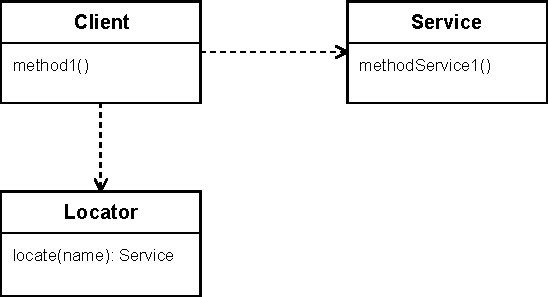
\includegraphics{figures/design-patterns-servicelocator.pdf}
    \caption{Service Locator}
    \label{fig:design-service-locator}
\end{figure}

The framework encourages the use of this pattern in all components. 
More specifically, the framework uses a Service Locator \fref{fig:design-service-locator} (called \texttt{injector}) to manage the responsibility of dependency creation.
Thus, services can be used in controllers and directives by their name.
The client class does not need to know the concrete implementation of the service. 
With this principle it is easy to mock classes for unit testing and change components in general.


\paragraph{Factory} Directives, controllers, services... are registered on modules. 
The \texttt{module.directive} \ac{API} registers them. 
It takes a normalised name and a factory function (\ref{fig:design-patterns-factory}) that returns an object with the fields that can be exposed to classes that use it.
For example, a Directive Definition Object or a Service.

\begin{figure}[htb]
    \centering
    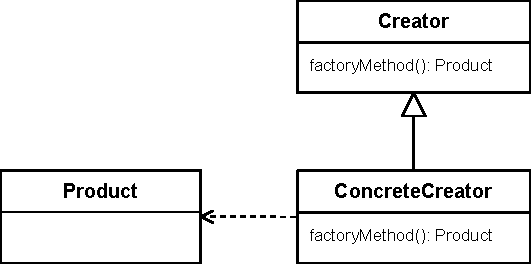
\includegraphics{figures/design-patterns-factory.pdf}
    \caption{Factory Method}
    \label{fig:design-patterns-factory0}
\end{figure}


\paragraph{Revealing Module} \cite{Osmani:2012} Modules typically help in having the units of code for a project separated.
JavaScript does not support the concept of classes but it does support special constructor functions that work with objects. 
The $new$ keyword used in a call to a constructor function makes JavaScript instantiate the new object with members defined by that function.
Modules are a way to emulate the concept of classes.
There are several options to implement them. 
This project uses object literal notation (CROSS REF JAVASCRIPT)
The module pattern encapsulates privacy, state and organisation using closures (CROSS REF JAVASCRIPT)
Only a public \ac{API} is returned, keeping everything else hidden within the closure private.
With the Revealing Module Pattern the code of the module is simplified: all variables and functions are defined in the private scope and returns an anonymous object with pointers to the private properties that should be revealed.
FIXME CROSS REF factory code example  + annotation "compare to writing the code of the function right there"

\paragraph{Remote Facade} FIXME: sure? do I have a remote facade in the app, in a controller? rosbridgectrl?

\paragraph{Command} 
Sometimes requests are issued to objects without knowing anything about the operation being requested or the receiver.
The command pattern is a behavioural design pattern in which an object is used to represent all the information needed to call a method at a later time. 
It lets objects make requests of unspecified application objects by turning the request itself into an object.
This object can be stored and passed around like other objects \cite{GoF:1995}.
Other names are \textbf{Transaction} or \textbf{Action Pattern}  

\fref{fig:design-command-general} shows the class diagram of this pattern in the context a traditional object-oriented programming language.
With JavaScript there are no abstract classes.
The approach that Osmani (\cite{Osmani:2012} proposes is having only concrete classes with a common \texttt{execute()} method.
\fref{sec:controllers} contains a description of the implementation in JavaScript of this pattern.

%design-command-1.js (and 2) are not used anymore

With a simple controller (\fref{fig:design-command-general}) one would call the methods in the object.
while this is correct, at the time the \ac{GUI} is built the \texttt{UI Component} does not know about the operations being requested.
For example, there is no way to define the behaviour for a \texttt{UI Component::Button} click handler.
Only the contents application knows it.
By adding an \texttt{execute} method to \texttt{ActionCtrl}, used in \texttt{UI Components} that accept the tag \texttt{onclick} and \texttt{action}, methods can be called without knowing them (\fref{fig:design-command-flango}).

\begin{figure}[htb]
    \centering
    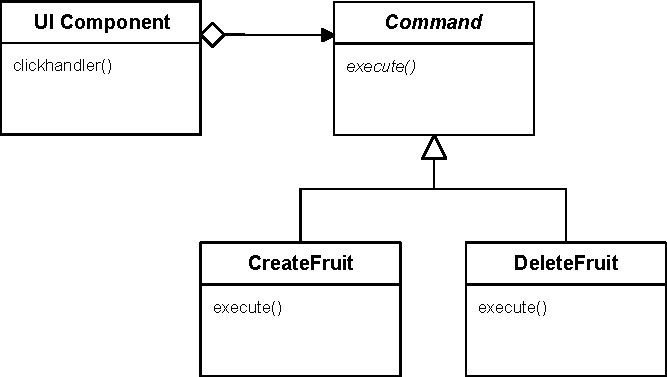
\includegraphics{figures/design-patterns-command-1.pdf}
    \caption{design patterns command 1}
    \label{fig:design-command-general}
\end{figure}

\begin{figure}[htb]
    \centering
    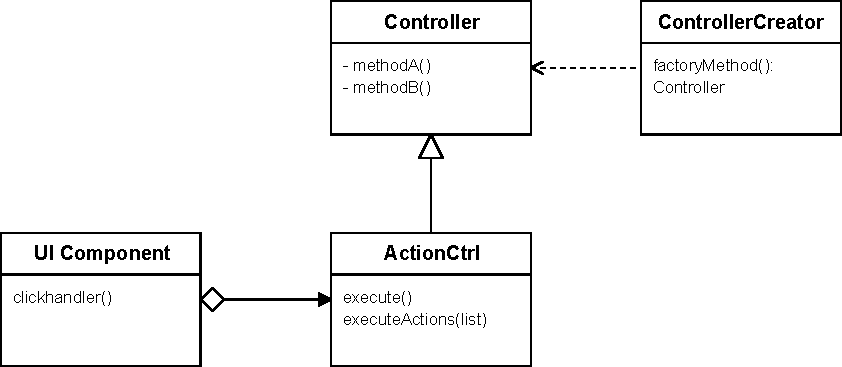
\includegraphics{figures/design-patterns-command-flango.pdf}
    \caption{design patterns command flango}
    \label{fig:design-command-flango}
\end{figure}

\subsection{Orientation to Web Components}
Web Components is a set of specifications that let web developers use \ac{HTML}, \ac{CSS} and JavaScript to build widgets that can be reused easily and reliably.
A web component consists of five pieces\cite{W3CComponents:2013}:
\begin{itemize}
    \item \textbf{Templates} define chunks of mark-up that are inert but can be activated for use later.
    \item \textbf{Decorators} apply templates based on CSS selectors to affect rich visual and behavioural changes to documents.
    \item \textbf{Custom Elements} let authors define their own elements, with new tag names and new script interfaces.
    \item \textbf{Shadow DOM}  encapsulates a DOM sub-tree for more reliable composition of user interface elements.
    \item \textbf{Imports} defines how templates, decorators and custom elements are packaged and loaded as a resource.
\end{itemize}

At the time of developing this project, the specification of web components is still a work in progress.
The technology, however, seems to fit in the needs of the project.
There are 2 well-known initiatives that implement an approach to web components: \textbf{Google Polymer} and \textbf{Google AngularJS}.

\paragraph{Polymer} Polymer is a framework that aims to use Web Components. 
It's based on Custom Elements, i.e. everything is a component.
With Polymer developers can compose and encapsulate bits of HTML that can be used in any other templating system or framework.
It uses \ac{HTML} and the \ac{DOM} \acp{API} to separate the view (\ac{DOM}) from the model. 
Updates to the model are reflected in the \ac{DOM} and user input in the view is immediately propagated to the model:: fast two-way data binding.

Polymer is in pre-alpha stage and can not be used in a stable project.
Angular, the framework of choice for this project, has features close to web components: it has declarative templates (in directives) that can be applied for elements, attributes, comments or classes (like Web Components decorators).
Directives are custom elements: behaviour can be placed in a directive controller, in a compile or in a link function.
Templates are usually \ac{HTML}, although it is not shadow \ac{DOM}.
Units of code can be grouped in modules, services, etc and be reused.

\FloatBarrier

\section{Static View}
the model, the view and the controllers. angualar modules, services, filters, controllers...
talk about the data model and \$rootScope ? talk about properties

un diagrama:
moduls, serveis, controladors, etc. 

This section contains a comprehensive description of the objects in the system and their relationships taking into account the technology that it uses: JavaScript and AngularJS client-side, Django in the backend, \ac{ROS} Topics to interoperate with the rest of the system.
There are two subsections: a class diagram and a packages diagram.

\subsection{Class Diagram}
JavaScript is an object-oriented language but it is not class-based.
It is prototype-based instead.
It can be used as a class-based language using constructors but this project does not need to do this: it does not create objects of any domain-specific class but, instead, uses the Angular constructs to instantiate services, controllers and directives, the building blocks of the application.
Most of boxes in these diagrams are not strictly classes but objects that are instantiated automatically by Angular.

% ********** CLASS DIAGRAM ********
\begin{figure}[htb]
    \centering
    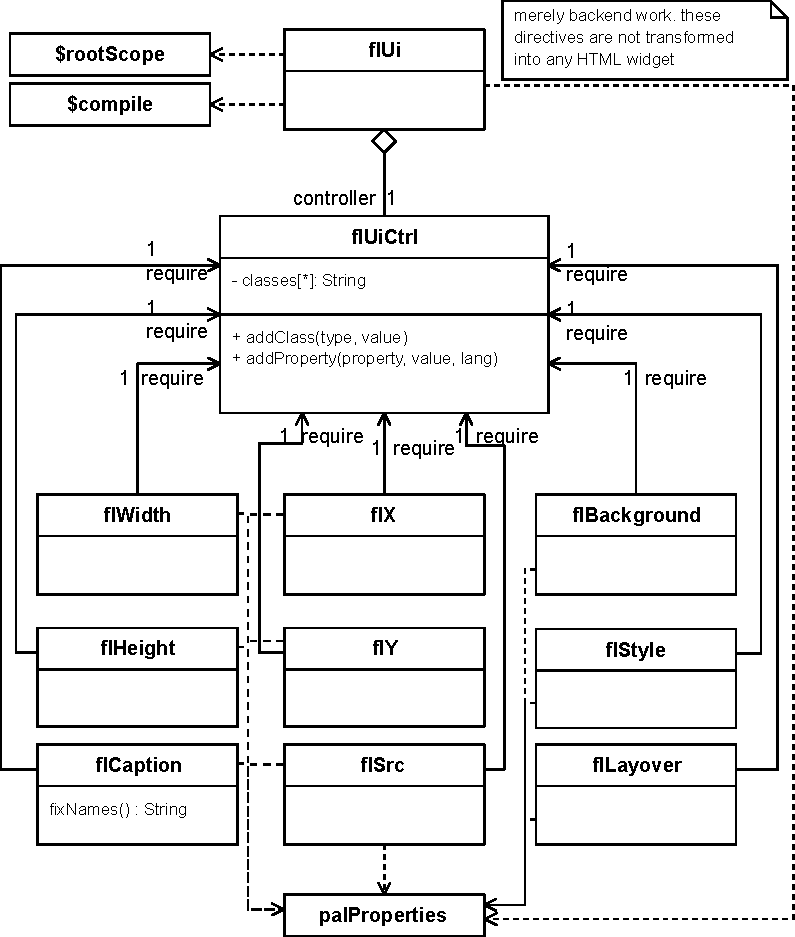
\includegraphics{figures/design-class-ui.pdf}
    \caption{Class Diagram -- UI}
    \label{fig:class-ui}
\end{figure}

\begin{sidewaysfigure}[htb]
    \centering
    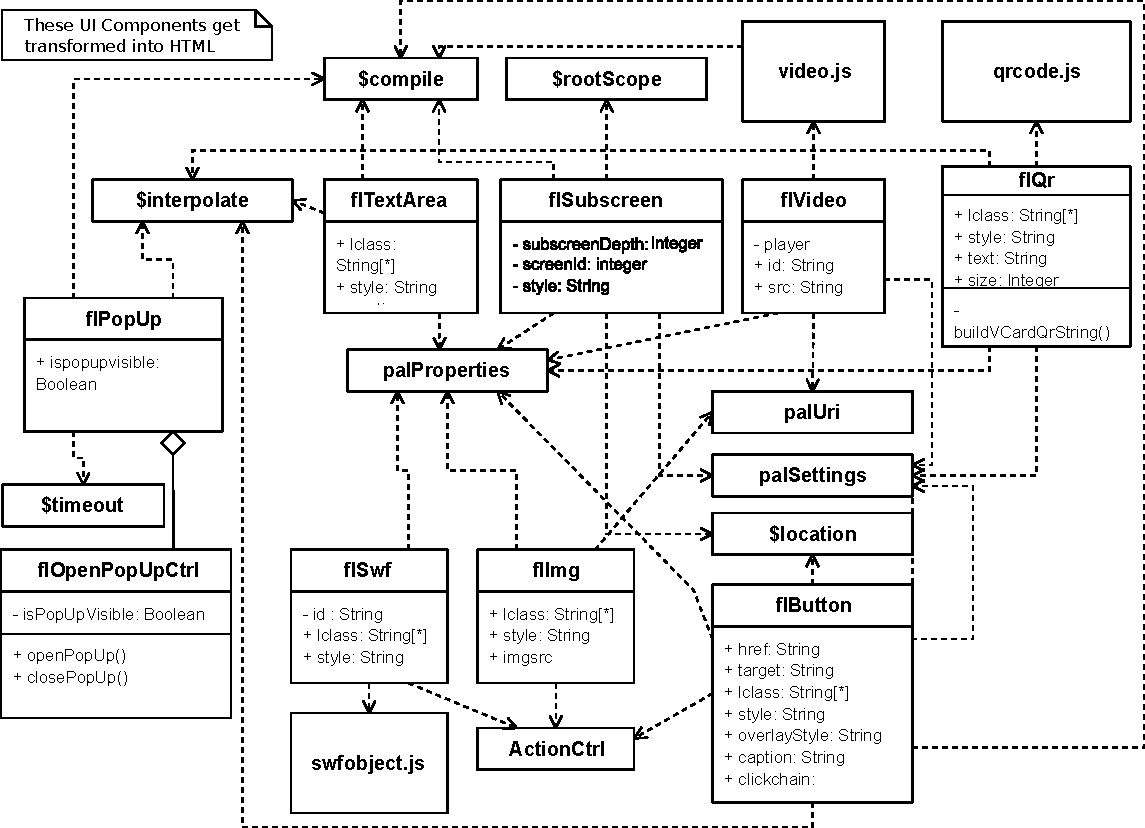
\includegraphics{figures/design-class-uicomponent.pdf}
    \caption{Class Diagram -- UI Component}
    \label{fig:class-uicomponent}
\end{sidewaysfigure}

\begin{sidewaysfigure}[htb]
    \centering
    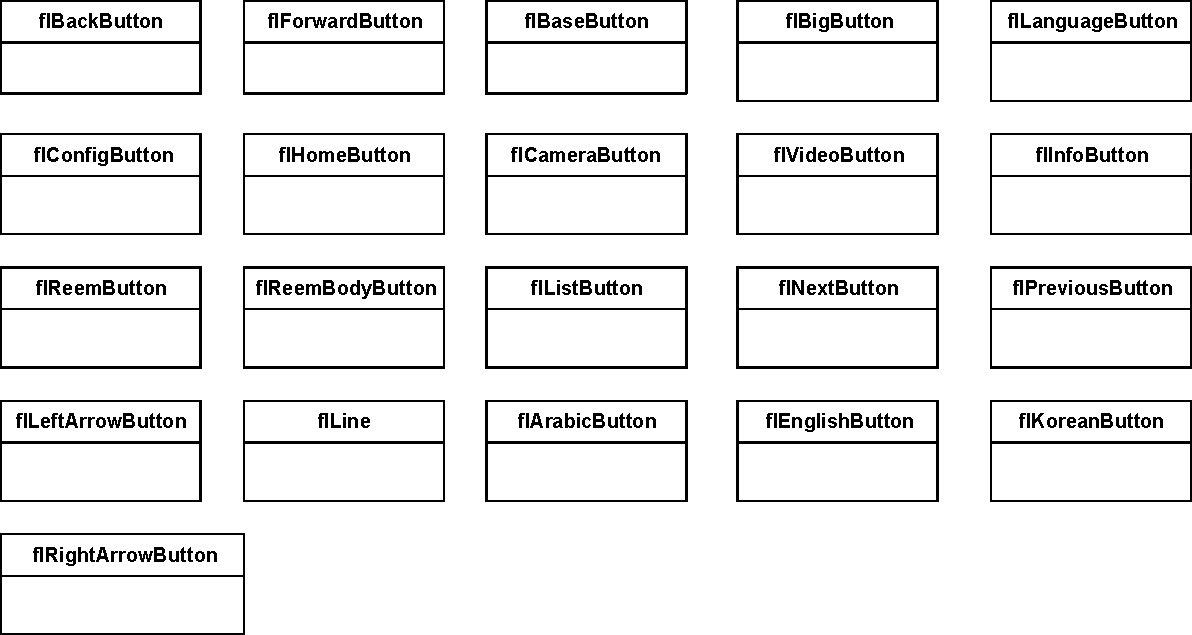
\includegraphics{figures/design-class-themecomponents.pdf}
    \caption{Class Diagram -- UI Theme Component}
    \label{fig:class-themecomponent}
\end{sidewaysfigure}

\begin{figure}[htb]
    \centering
    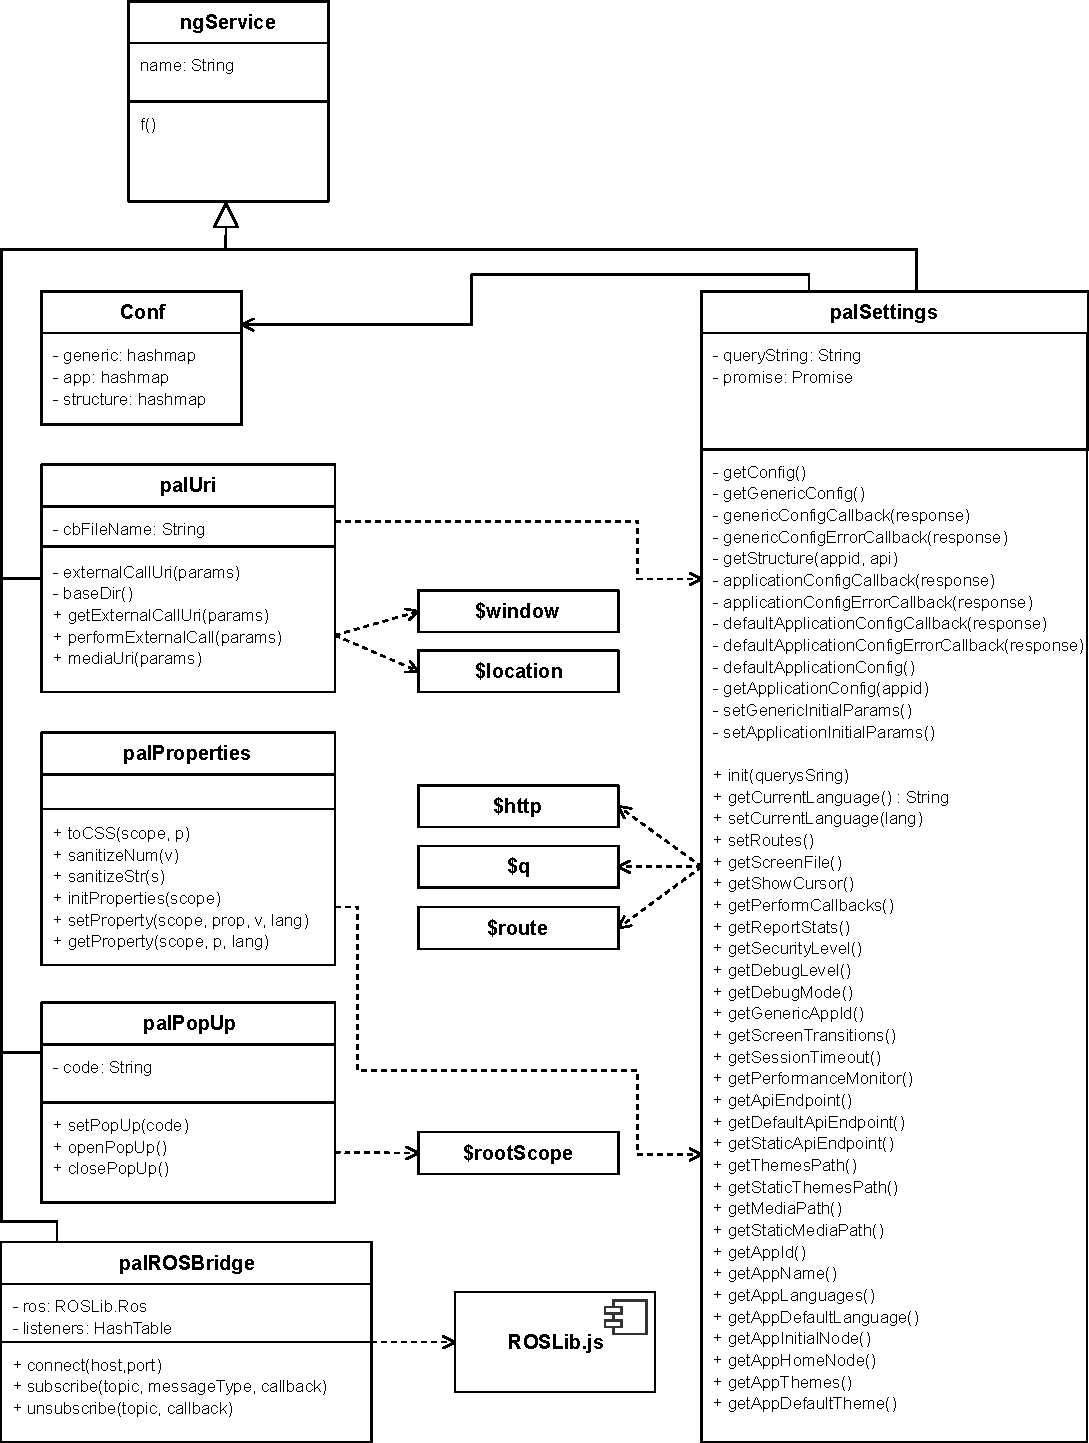
\includegraphics{figures/design-class-services.pdf}
    \caption{Class Diagram -- UI services}
    \label{fig:class-services}
\end{figure}

\begin{figure}[htb]
    \centering
    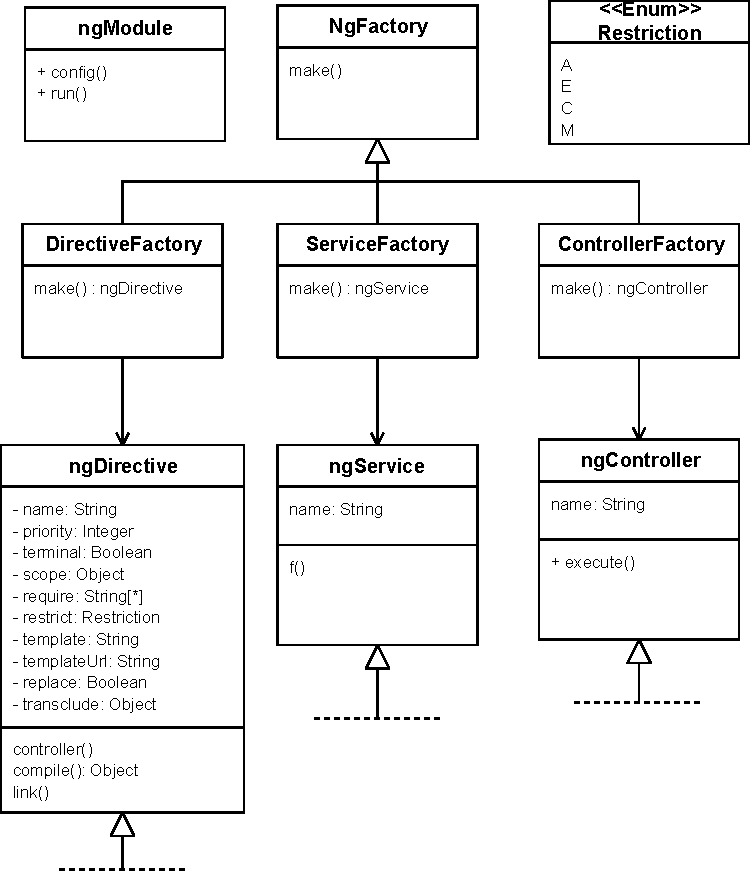
\includegraphics{figures/design-class-ngfactory.pdf}
    \caption{Class Diagram -- angular factory}
    \label{fig:class-ngfactory}
\end{figure}

\begin{figure}[htb]
    \centering
    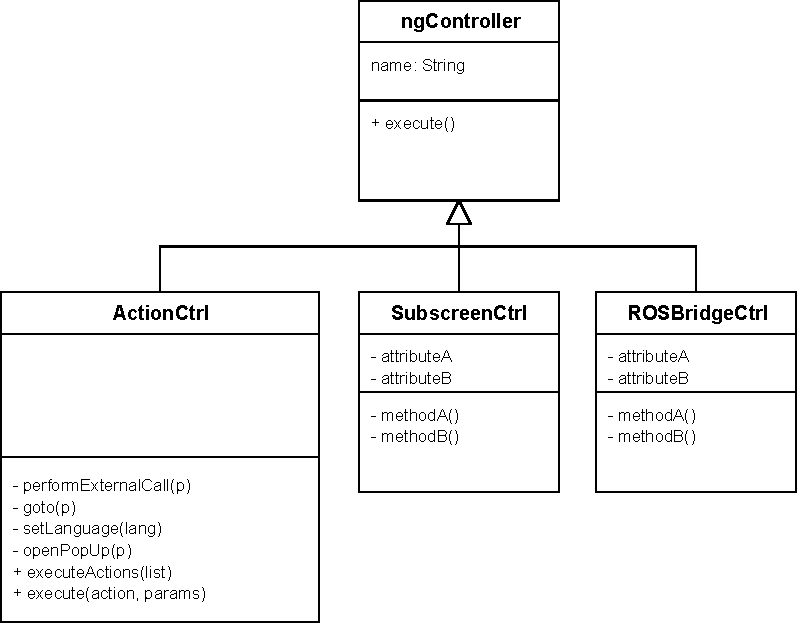
\includegraphics{figures/design-class-controllers.pdf}
    \caption{Class Diagram -- angular controllers}
    \label{fig:class-controllers}
\end{figure}

\begin{figure}[htb]
    \centering
    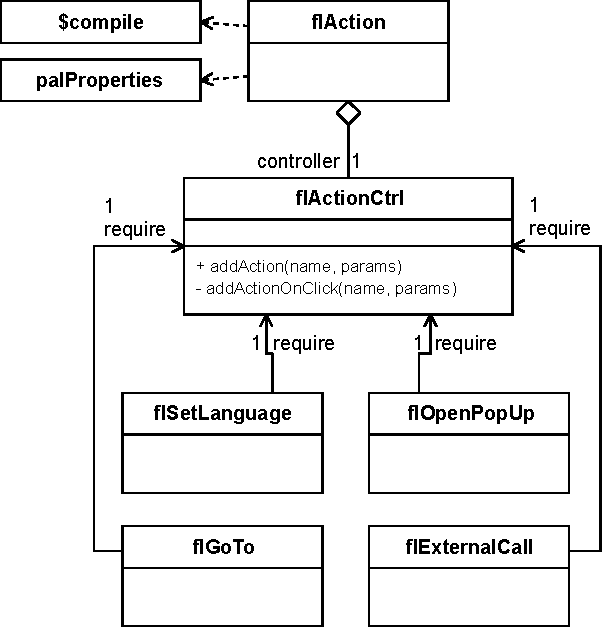
\includegraphics{figures/design-class-action.pdf}
    \caption{Class Diagram -- ui action}
    \label{fig:class-action}
\end{figure}


% ********** PACKAGE DIAGRAM ********
\FloatBarrier
\subsection{Packages Diagrams}

\begin{figure}[htb]
    \centering
    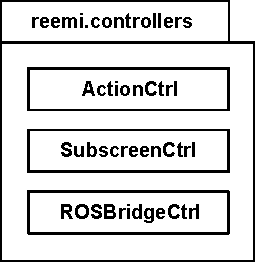
\includegraphics{figures/design-package-controllers.pdf}
    \caption{Packages Diagram -- controllers}
    \label{fig:pkg-controllers}
\end{figure}

\begin{figure}[htb]
    \centering
    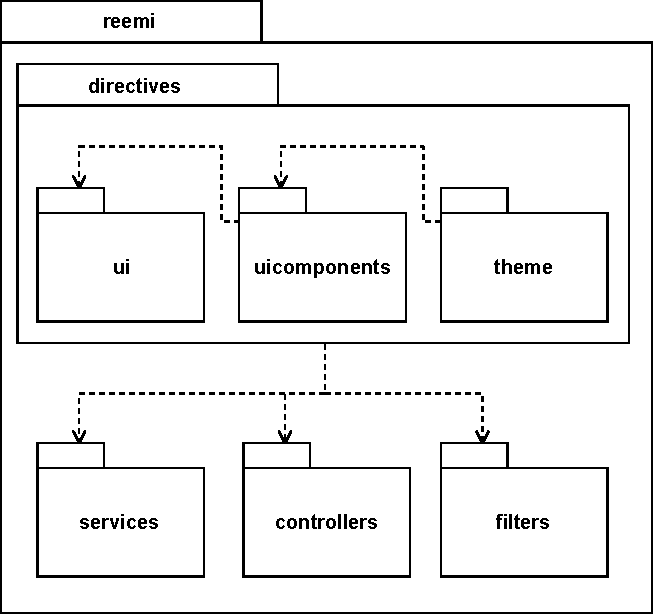
\includegraphics{figures/design-package-reemi.pdf}
    \caption{Packages Diagram -- application}
    \label{fig:pkg-reemi}
\end{figure}

\begin{figure}[htb]
    \centering
    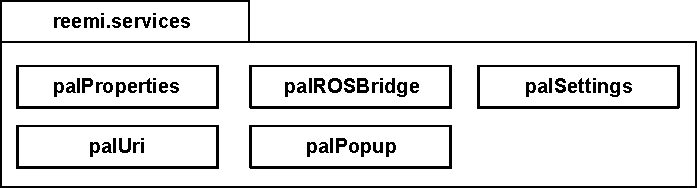
\includegraphics{figures/design-package-services.pdf}
    \caption{Packages Diagram -- services}
    \label{fig:pkg-services}
\end{figure}

\begin{figure}[htb]
    \centering
    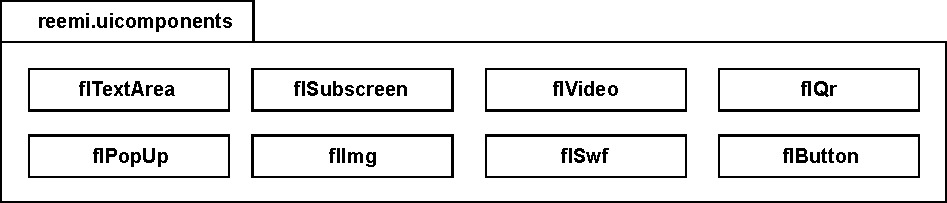
\includegraphics{figures/design-package-uicomponents.pdf}
    \caption{Packages Diagram -- UI components}
    \label{fig:pkg-uicomponents}
\end{figure}

\begin{figure}[htb]
    \centering
    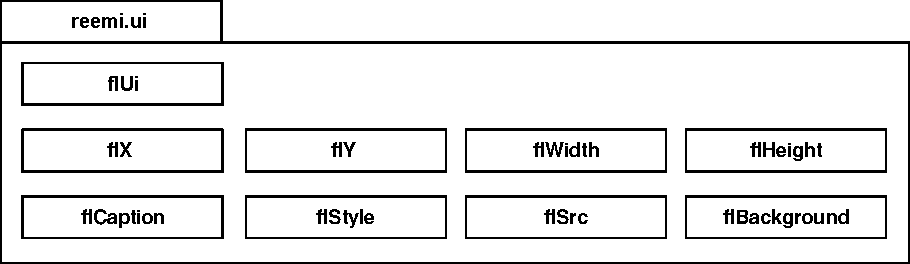
\includegraphics{figures/design-package-ui.pdf}
    \caption{Packages Diagram -- UI}
    \label{fig:pkg-ui}
\end{figure}

\begin{figure}[htb]
    \centering
    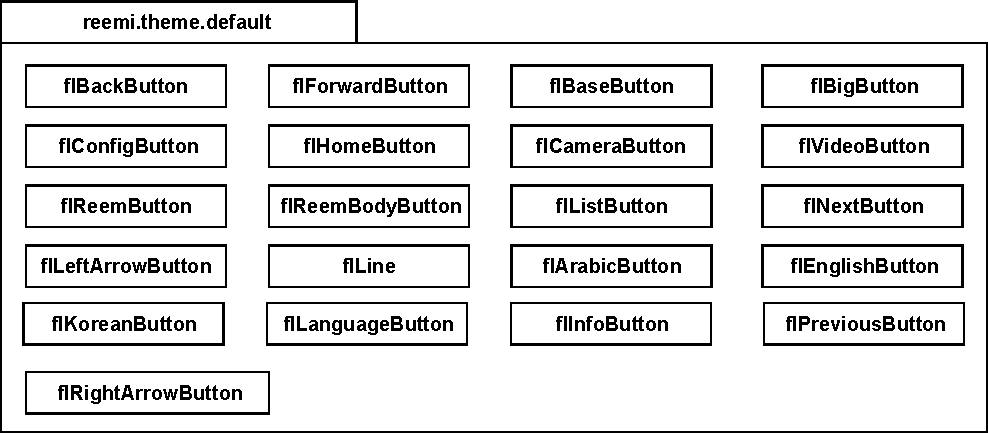
\includegraphics{figures/design-package-uithemecomponents.pdf}
    \caption{Packages Diagram -- UI theme components}
    \label{fig:pkg-themecomponents}
\end{figure}

\FloatBarrier

\section{Dynamic view}
the flow: user creates an application, [robot sync], my app reads it and generates HTML output.

specific flow of an app. bootstrap, the compile-link phase, push classes, push styles, get url params, etc.
examples of using the properties, generating the settings, fetching things from the server, rostopics...

show patterns!

This section contains a detailed description of the most relevant operations.
They are grouped in XXX categories: boot-strap and configuration, handling properties and transformation to \ac{HTML}, pop-ups, internal navigation and communication with ROS Bridge.
It always works the same way: writing the appropriate behaviour in directives (controller, compile and link functions) and injecting the required services following the flow that Angular needs.

\subsection{Overview}
compile-link-ctrl
seq diagram: detecting a directive, etc. general example with "book" "fruit" etc

\subsection{Boot-strap and Configuration}
FIXME Notes: description -- bootup (register modules, fetch config, querystring, goto init, subscribe)

Some key operations are done during the boot-strap process of Angular, like registering modules, setting dependencies and the default routes (e.g. \texttt{http:// ... /app/index.html\#/products-view/14/detail-view}.
The Flango \cm also fetches de configuration from the backend and builds the local object that represents it.
Figures \fref{fig:design-seqdia-bootstrap-1}, \fref{fig:design-seqdia-bootstrap-2} and \fref{fig:design-seqdia-bootstrap-3}, show the bootstrap of the program.

\begin{figure}[htb]
    \centering
    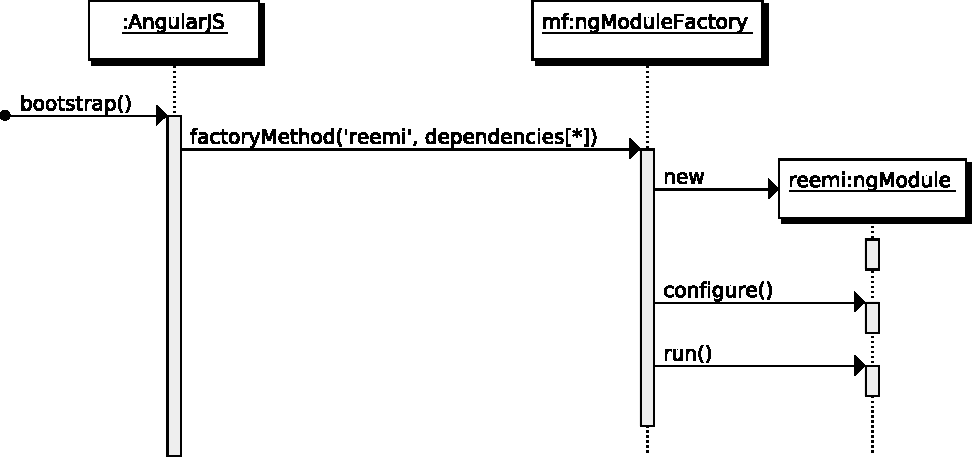
\includegraphics{figures/design/seqdia/bootstrap-1.pdf}
    \caption{Bootstrap 1}
    \label{fig:design-seqdia-bootstrap-1}
\end{figure}

\begin{figure}[htb]
    \centering
    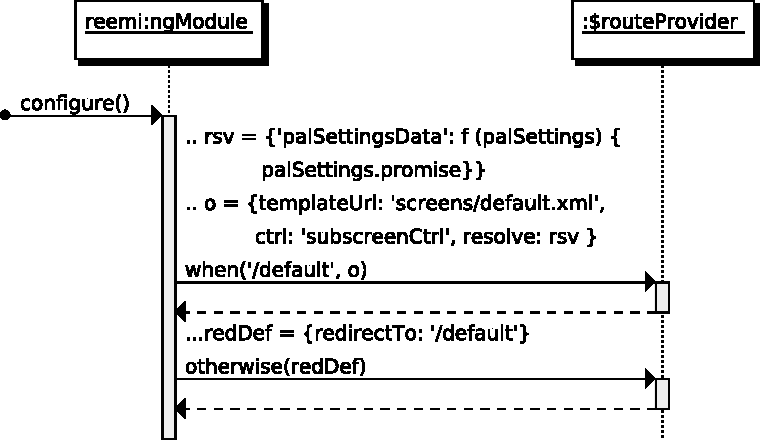
\includegraphics{figures/design/seqdia/bootstrap-2.pdf}
    \caption{Bootstrap 2}
    \label{fig:design-seqdia-bootstrap-2}
\end{figure}

\begin{figure}[htb]
    \centering
    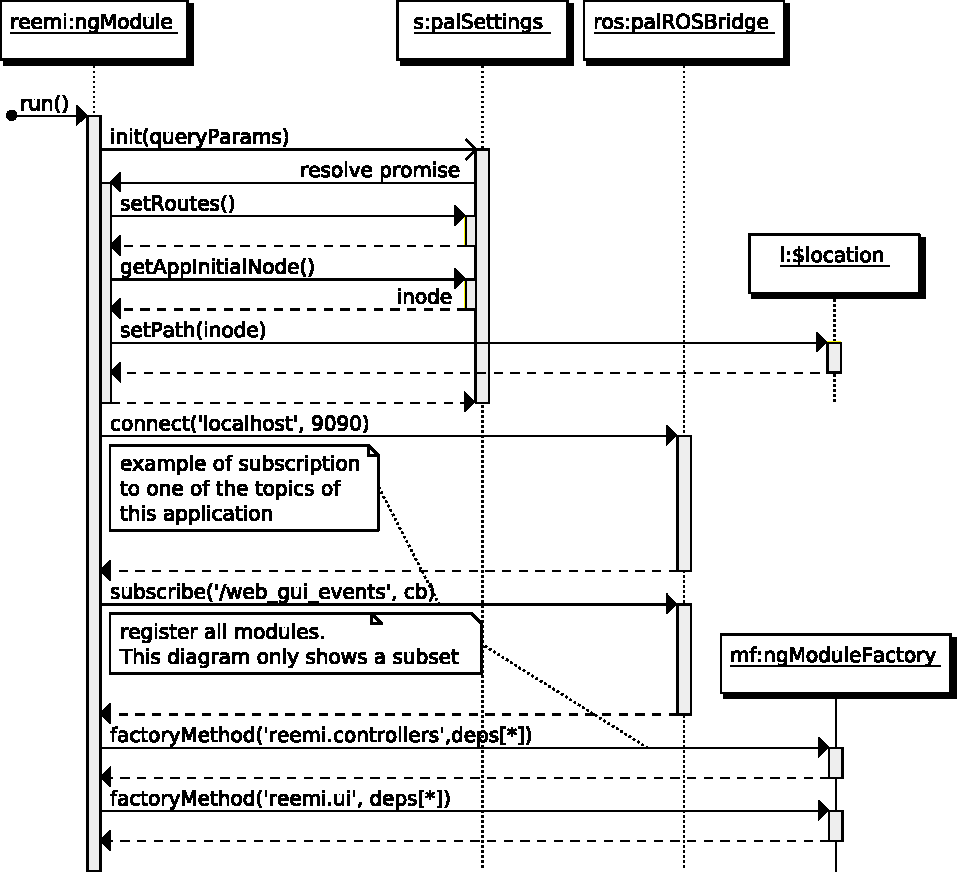
\includegraphics{figures/design/seqdia/bootstrap-3.pdf}
    \caption{Bootstrap 3}
    \label{fig:design-seqdia-bootstrap-3}
\end{figure}

The configuration is encapsulated in the \texttt{palSettings} angular service which, like all services in Angular, is a singleton.
This service is created with a factory: when a new instance of palSettings is to be created, it runs some code that prepares an object to return, the instance itself.
It is instantiated and initialised the first time it is called.
The configuration object is created during the bootstrap.
It calls \lstinline$palSettings.init(queryString)$ \fref{fig:design-seqdia-palSettings-init}.
This method fetches the configuration from the backend using an asynchronous call (\fref{fig:design-seqdia-palSettings-getConfig}) which, in turn, delegates to other internal operations.
To avoid errors, the system uses \emph{deferred promises}: the \texttt{init} method returns an object immediately and it receives a notification when all asynchronous calls have been completed, that is, when the configuration object is ready to be used in the application.

The configuration object has three parts: the generic configuration (paths, \ac{API} endpoint, etc) \fref{fig:design-seqdia-palSettings-getGenericConfig}, the application specific configuration {fig:design-seqdia-palSettings-getApplicationConfig} (available languages, available themes, default language, etc) and the structure \fref{fig:design-seqdia-palSettings-getStructure} (a graph that matches screens with \ac{URI}.
It degrades gradually: it first tries to fetch the real application, if it fails attempts to fetch the default application \fref{fig:design-seqdia-palSettings-defaultApplicationConfig}, if this is not possible, it obtains the static application shipped with the program (See \texttt{errorCallback} in \fref{fig:design-seqdia-palSettings-defaultApplicationConfig}).

\paragraph{Promises and deferred objects} Futures, promises and delays are constructs for synchronising in a programming language.
\textit{Promises} were introduced by Daniel P. Friedman and David Wise in 1977, \textit{futures} in 1977 by Henry Baker and Carl Hewitt.
The term promise was coined by Liskov and Shrira (\cite{Liskov:1988}) in 1988.

The three words are often used interchangeably although they have some differences:
\begin{itemize}
\item Future: read-only placeholder view of a variable
\item Promise: writeable, single assignment container that sets the value of the future.
\end{itemize}
Essentially, promises represent the result of a task that might have not been completed, something very common in JavaScript.
Asynchronous calls are normally handled with callbacks (FIXME see chapter 7 for impl).
However, when there are nested or concurrent asynchronous calls, like the case of fetching the configuration from the \flangobe , callbacks become hard to maintain.
A solution is defining a promise at the beginning and \emph{resolving} it when all calls are completed (or \emph{rejecting} it when a sufficient number of calls have failed).
This way functions can be decoupled and testing is easier. 

\begin{figure}[htb]
    \centering
    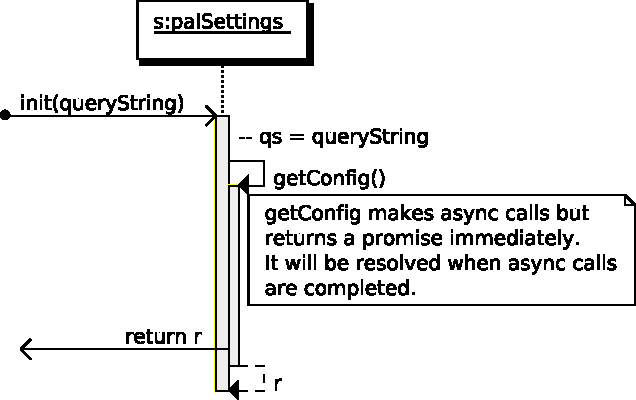
\includegraphics{figures/design/seqdia/palSettings-init.pdf}
    \caption{init()}
    \label{fig:design-seqdia-palSettings-init}
\end{figure}

\begin{figure}[htb]
    \centering
    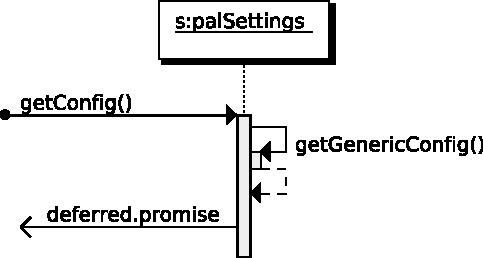
\includegraphics{figures/design/seqdia/palSettings-getConfig.pdf}
    \caption{getConfig()}
    \label{fig:design-seqdia-palSettings-getConfig}
\end{figure}

\begin{figure}[htb]
    \centering
    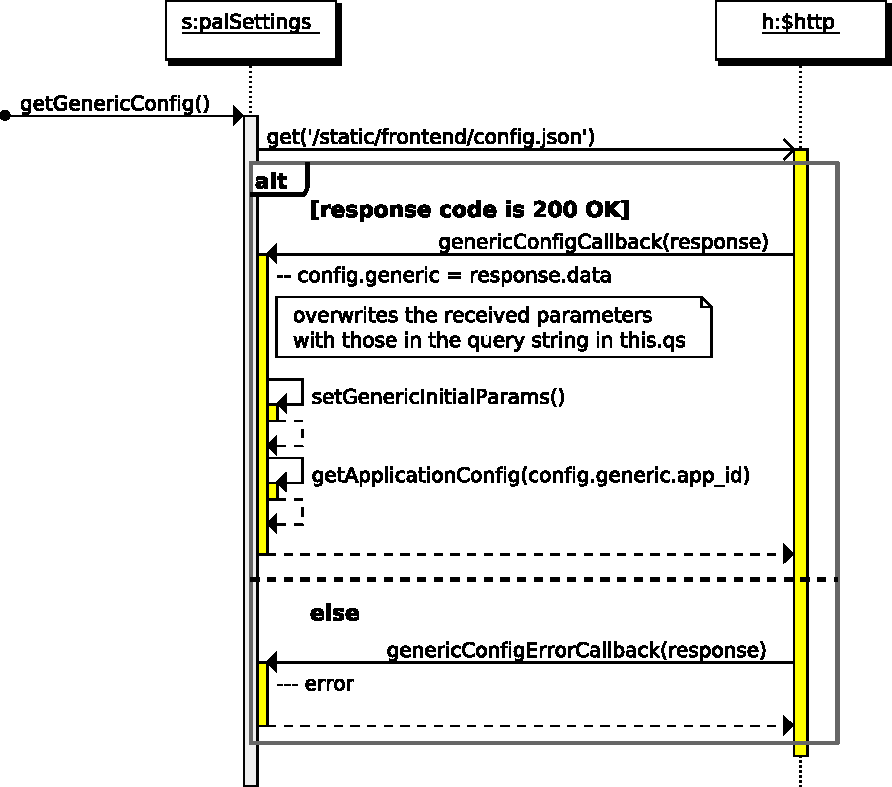
\includegraphics{figures/design/seqdia/palSettings-getGenericConfig.pdf}
    \caption{getGenericConfig()}
    \label{fig:design-seqdia-palSettings-getGenericConfig}
\end{figure}

\begin{figure}[htb]
    \centering
    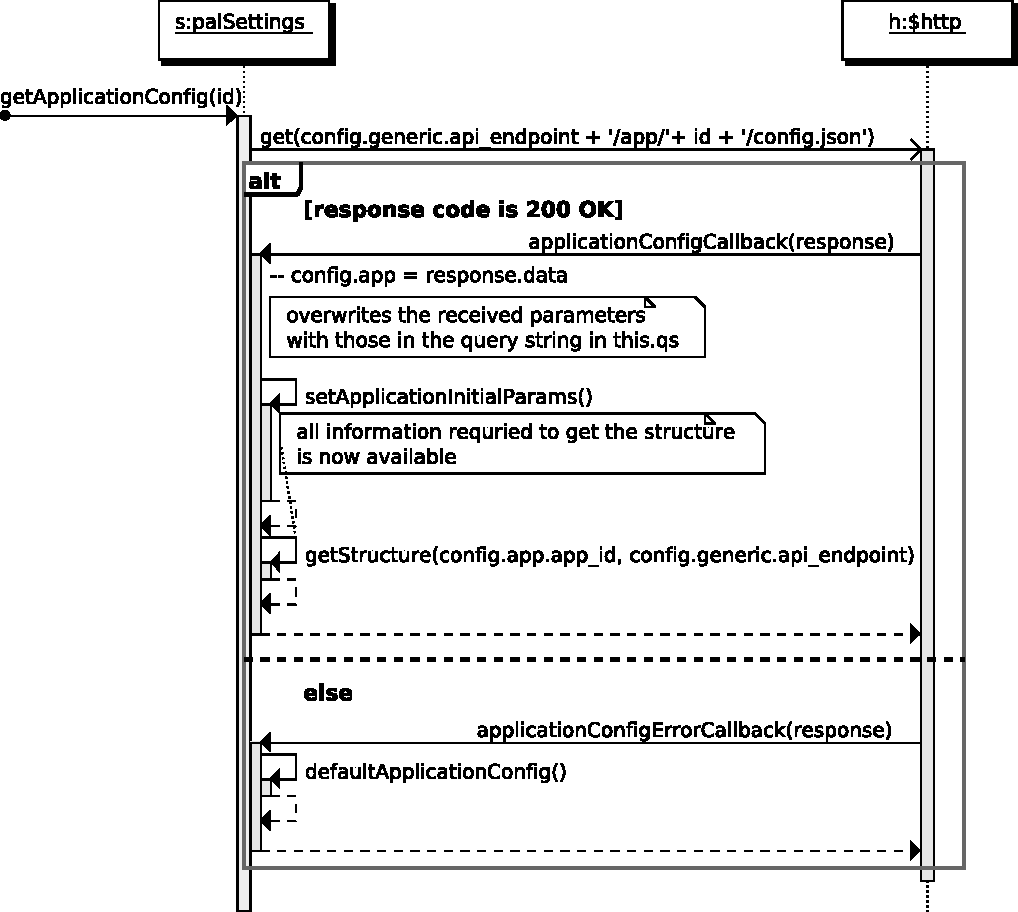
\includegraphics{figures/design/seqdia/palSettings-getApplicationConfig.pdf}
    \caption{getApplicationConfig()}
    \label{fig:design-seqdia-palSettings-getApplicationConfig}
\end{figure}


\begin{figure}[htb]
    \centering
    \includegraphics{figures/design/seqdia/palSettings-getStructure.pdf}
    \caption{getStructure()}
    \label{fig:design-seqdia-palSettings-getStructure}
\end{figure}

\begin{sidewaysfigure}[htb]
    \centering
    \includegraphics{figures/design/seqdia/palSettings-defaultApplicationConfig.pdf}
    \caption{defaultApplicationConfig()}
    \label{fig:design-seqdia-palSettings-defaultApplicationConfig}
\end{sidewaysfigure}

\FloatBarrier

\subsection{Properties management and transformation to \ac{HTML}}
descr with example (transform a  book into...)

interpretacio de tags. fl:ui type=.. --> fl {type} per separar

herència de ui components (un basebutton s'implementa amb...)

plantilles dels temes

Browsers can only parse \ac{HTML} nodes.
When the parser finds an \ac{XML} node, it prints the inner text node because \ac{HTML} also has text nodes.
With Angular \ac{XML} nodes can have behaviour: it teaches the browser new syntax.
For example, \lstinline$<fl:ui fl:base-button fl:x="100" fl:width="90"></ui>$ triggers the directive \lstinline$flBaseButton$, which encapsulates the behaviour to transform it to \ac{HTML}: \lstinline$<a href="..."><div>text</div></a>$.

To expose values to the view, Angular attaches an object \texttt{\$scope} to all directives  \fref{fig:design-properties-management}.
A scope can be \textbf{isolated}, \textbf{prototypically inherited} from the parent, or \textbf{shared} with other directives of the same type.
This project uses the scope to encapsulate the properties extracted or inferred from the \ac{XML} node.
Thus, any element \lstinline$<fl:ui>$ or concrete types \lstinline$base-button$, \lstinline$back-button$, etc has a \texttt{scope} object attached that contains all the necessary data to render an \ac{HTML} node.
Scopes are also watched to provide two-way data binding with controllers (see CROSS REF observer/mvc)

\begin{figure}[h]
    \centering
    \includegraphics{figures/design/properties-management.pdf}
    \caption{Scope object attached to a node}
    \label{fig:design-properties-management}
\end{figure}

\lstinputlisting[language=xml, caption={Original XML BaseButton}, label="design-real-xml-button"]{src/from-xml-to-html-1.xml}
\lstinputlisting[language=JavaScript, caption={Properties object}, label="design-scope-properties"]{src/from-xml-to-html-properties.js}

\begin{figure}
    \centering
    \includegraphics{figures/design/from-xml-to-html-3.pdf}
    \caption{Transformation from XML to HTML and styles management}
    \label{fig:design-xml-to-html-3}
\end{figure}


Directives can be \textbf{restricted} to \textbf{Element}, \textbf{Attribute}, \textbf{Class} or \textbf{coMment} \fref{fig:class-ngfactory}.
Flango \cm is designed to adapt to this syntax and to decouple and reuse elements as much as possible.
All UI Components have the tag \lstinline$<fl:ui>$ and an attribute \lstinline$fl:type$ that defines the concrete type.
Instead of having all behaviour in one directive \texttt{fl:ui} (restricted to Element), it uses \texttt{flUi} to rewrite the \ac{DOM}: \lstinline$<fl:ui fl:type="base-button"></ui>$ becomes \lstinline$<fl:ui base-button></ui>$, where \texttt{base-button} is an attribute of the element \texttt{fl:ui}.
There is a directive \texttt{flBaseButton} (restricted to Attribute) that encapsulates the behaviour of this tag.
Likewise, it initialises the properties object for this \texttt{ui} element and stores the type that will be later used as a value for the \texttt{class} attribute in the \ac{HTML} element.
The stylesheet of the theme defines the inheritance of styles: a base-button is implemented with a button and, therefore, inherits all properties of the class \texttt{button}.

Figure \fref{fig:design-xml-to-html-3} shows the implementation of the transformation the base button in the \ac{XML} screen (\ref{design-real-xml-button}) and the use of the properties object in the scope (\ref{fig:design-xml-to-html-3}).

The algorithm to decide the properties for an object and draw it with \ac{HTML} goes with the flow of the framework:
\begin{enumerate}
	\item With directive \texttt{flUi}: Create an attribute with the value of the \texttt{type} attribute \fref{fig:design-seqdia-ui-compile}. Initialise the properties object in the controller \fref{fig:design-seqdia-ui-controller} The framework compiles and links the rest of the code (e.g. the \texttt{link()} function in inner \texttt{width} tags to read values of inner tags (\fref{fig:design-seqdia-width-link}))
	\item With directive \texttt{flUi} link function (\fref{fig:design-seqdia-ui-link}), read in-line attributes. Because it reads everything recursively, this is the last function to run. Properties are only set if they have not been set yet: inner tags (more specific) have higher priority than in-line attributes. Recompile the directive to make angular find it. 
	\item With the new directive (e.g. \texttt{flBaseButton}), run component-specific behaviour. \texttt{flUi} does not have a \texttt{type} attribute anymore and is ignored. Specific behaviour can be transforming it using a template \fref{fig:design-seqdia-basebutton-link}. Recompile (e.g. the template might, and normally has, tags that can trigger angular directives).
	\item Eventually reach a base component and run component-specific behaviour, e.g. create \ac{HTML} nodes that can actually draw the UI Component.
\end{enumerate}

\begin{figure}[htb]
    \centering
    \includegraphics{figures/design/seqdia/ui-compile.pdf}
    \caption{flUi::compile}
    \label{fig:design-seqdia-ui-compile}
\end{figure}

\begin{figure}[htb]
    \centering
    \includegraphics{figures/design/seqdia/ui-controller.pdf}
    \caption{flUi::controller}
    \label{fig:design-seqdia-ui-controller}
\end{figure}

\begin{figure}[htb]
    \centering
    \includegraphics{figures/design/seqdia/width-link.pdf}
    \caption{flWidth::link}
    \label{fig:design-seqdia-width-link}
\end{figure}

\begin{figure}[htb]
    \centering
    \includegraphics{figures/design/seqdia/ui-link.pdf}
    \caption{flUi::link}
    \label{fig:design-seqdia-ui-link}
\end{figure}

\begin{figure}[htb]
    \centering
    \includegraphics{figures/design/seqdia/basebutton-link.pdf}
    \caption{flBaseButton::link}
    \label{fig:design-seqdia-basebutton-link}
\end{figure}

\lstinline$<fl:ui base-button></ui>$ eventually becomes \lstinline$<div class="base-button" style="..."><div class="caption">Hello World</caption></div>$. 
With this rewrite strategy the directive eventually outputs real \ac{HTML} that defines the structure of the UI Component and uses the style sheet.

All UI Components have an  \textbf{\ac{HTML} template} that defines their structure, a \textbf{\ac{CSS} class} that defines their style, \textbf{in-line \ac{CSS}} that defines their exclusive properties (e.g. position, size...) and they are binded to \textbf{\texttt{ActionCtrl}} to expose behaviour (e.g. on click).
\FloatBarrier

\paragraph{Inheritance and composition} UI Components can be composited: a \texttt{home-button} is implemented with a \texttt{base-button}, which in turn it is implemented with a \texttt{button}, that eventually becomes \ac{HTML}.
Each component can have defaults for properties.
For instance, if \texttt{base-button} has a \texttt{width} of 100px in the template, and a component that is implemented with \texttt{base-button} (e.g. \texttt{home-button}) does not define a different with, it sets \texttt{with} to 100 in the properties object.
This behaviour is achieved with the \texttt{compile} and \texttt{link} functions of directives.
Language-specific properties are decided the same way: it attempts to use current language properties, if they are not defined, it falls back to the default language.

\subsection{Actions execution}
Buttons and other UI Components, like images or QR Codes, respond to clicks.
\ac{XML} can define a list of actions to execute (e.g. set the language, open a popup, go to \ac{URI}...)
The controller ActionCtrl encapsulates the logic to process these commands.

\lstinputlisting[language=xml, caption={A list of actions}]{src/example-actions.xml}

\lstinputlisting[language=html, caption={Result button (snippet)}]{src/example-result-button.html}

To create the list of actions, when the component is clicked it runs \lstinline$executeActions()$, which has a list of actions to execute as a parameter using the command pattern.

\begin{figure}[htb]
    \centering
    \includegraphics{figures/design/seqdia/actionCtrl-executeActions.pdf}
    \caption{ActionCtrl::executeActions}
    \label{fig:design-seqdia-actionCtrl-executeActions}
\end{figure}

\begin{figure}[htb]
    \centering
    \includegraphics{figures/design/seqdia/actionCtrl-execute.pdf}
    \caption{ActionCtrl::execute}
    \label{fig:design-seqdia-actionCtrl-execute}
\end{figure}


\begin{figure}[htb]
    \centering
    \includegraphics{figures/design/seqdia/actionCtrl-goto.pdf}
    \caption{ActionCtrl::execute}
    \label{fig:design-seqdia-actionCtrl-goto}
\end{figure}

\FloatBarrier

\subsection{Pop-Ups}
description and use example

\subsection{Internal Navigation}
Angular has a navigation system based on the \acp{URL}.
The \$route service has a map that relates \acp{URL} with screens, \ac{HTML} files with directives.
On each location change, Angular looks up the destination \ac{URL} in the map to fetch the correct file.

Flango \cm composites screens with subscreens and decides the contents to show using the \ac{URL} \fref{fig:design-internal-navigation}.
e.g. the \ac{URL} \texttt{/main-view/animals-list} does not populate the subscreen \texttt{red-panda-details}

\begin{figure}[htb]
    \centering
    \includegraphics{figures/design/internal-navigation.pdf}
    \caption{Screens and subscreens for internal navigation}
    \label{fig:design-internal-navigation}
\end{figure}

The behaviour of subscreens is defined in the \texttt{subscreen} directive (\fref{fig:design-seqdia-subscreen-compile}).

Only after properties of the UI Component Subscreen have been set (and the corresponding \ac{HTML} element created), Angular includes the file of the subscreen.

\begin{sidewaysfigure}[htb]
    \centering
    \includegraphics{figures/design/seqdia/subscreen-compile.pdf}
    \caption{Subscreen::compile}
    \label{fig:design-seqdia-subscreen-compile}
\end{sidewaysfigure}

\FloatBarrier

\subsection{External Calls}
motivation, rosbridge

\subsection{Responding to requests from the robot}
service, topic, rosbridge, etc

\begin{figure}[htb]
    \centering
    \includegraphics{figures/design/seqdia/ROSBridgeCtrl-creation.pdf}
    \caption{ROSBridgeCtrl::instantiation and subscription to topic}
    \label{fig:design-seqdia-ROSBridgeCtrl-creation}
\end{figure}

\begin{sidewaysfigure}[htb]
    \centering
    \includegraphics{figures/design/seqdia/ROSBridgeCtrl-callback.pdf}
    \caption{ROSBridgeCtrl::Example callback function}
    \label{fig:design-seqdia-ROSBridgeCtrl-callback}
\end{sidewaysfigure}

\FloatBarrier

\section{Physical view}
This section presents a series of diagrams to illustrate the physical layout of the project: the nodes involved, the components in each node, and a clear separation of the Flango \cm and the environment.
The application is assembled in a Debian package and deployed to Basestation and the robot.
The control scripts of this package perform tasks like copying the files to the correct place (e.g. the public html folder of the web server), initialise data in the backend, etc.
The diagrams in this section show the system after the installation.

% ****** deployment *******
\begin{figure}[htb]
    \centering
    \includegraphics{figures/design-deployment-basestation.pdf}
    \caption{Deployment Diagram -- basestation}
    \label{fig:deploy-basestation}
\end{figure}

\begin{sidewaysfigure}[htb]
    \centering
    \includegraphics{figures/design-deployment-browser.pdf}
    \caption{Deployment Diagram -- browser}
    \label{fig:deploy-browser}
\end{sidewaysfigure}

\begin{figure}[htb]
    \centering
    \includegraphics{figures/design-deployment-mediacomputer.pdf}
    \caption{Deployment Diagram -- media computer}
    \label{fig:deploy-media}
\end{figure}

\begin{figure}[htb]
    \centering
    \includegraphics{figures/design-deployment-reem.pdf}
    \caption{Deployment Diagram -- reem}
    \label{fig:deploy-reem}
\end{figure}

\begin{figure}[htb]
    \centering
    \includegraphics{figures/design-deployment-webserver.pdf}
    \caption{Deployment Diagram -- webserver}
    \label{fig:deploy-webserver}
\end{figure}

\FloatBarrier

FIXME MAYBE ADD NETWORK DIAGRAM? VPN, ENCRIPTION? it's qutie simple % design
\chapter{Implementation}
\label{chap:implementation}
This chapter describes the environment to develop and run Flango \cm and the implementation of the key features.

\section{Development environment set-up}
Flango \cm belongs to a bigger project.
The development environment is adapted to this situation to ensure a correct integration.
Moreover, the project uses tools to run unit tests, generate code, etc.

\subsection{Integration}
The files of Flango \cm live in the server as part of the \flangobe .
The backend is developed with Django and requires a set of Python libraries that might not be available in the system.
To overcome this situation, Flango is developed in a virtual environment and files are made available to clients with the built-in web server in Django, although Basestation uses Apache2 and the robot Lighttpd.
All the code is in a subversion repository.

\begin{lstlisting}[caption=lalala, label=virtual-env]
$ mkvirtualenv local-flango
$ workon local-flango
$ pip install --upgrade -r requirements.txt
\end{lstlisting}

Virtual environments have pre and postactivate scripts to alter the default behaviour.
Flango needs to modify environment variables to make \texttt{local-flango} live in the local copy of the repository, use a database, set aliases, etc.

After the virtual environment is ready, it is easier to change between branches.
Django is one of the packages available in the virtual environment and has a built-in web server to develop that runs on port 8000.

\begin{lstlisting}[caption=Django web server, label=virtual-env-server]
~/contentMgmtBranches/trunk/backend$ django runserver
Validating models...

modeltranslation: Registered 0 models for translation () [pid: 5286].
0 errors found
Django version 1.4.3, using settings 'flango.settings'
Development server is running at http://127.0.0.1:8000/
Quit the server with CONTROL-C.

"GET /static/flangoh/flangoh/app/index.html HTTP/1.1" 200 2317
\end{lstlisting}

The file structure of the whole project is shown in listing \ref{impl-flango-files-layout}.
Folders \texttt{build}, \texttt{packaging} and \texttt{conf} contain scripts to build Debian packages to deploy the software on the robot and basestation.
\texttt{src} contains the \flangobe , which includes the \flangofe (and the \se).
The project of this thesis, Flango \cm is in the \texttt{static} folder (\ref{impl-flango-static-files-layout}), that contains files served without any processing server-side.

\begin{lstlisting}[columns=fixed,caption=Flango files layout, label=impl-flango-files-layout]
~/contentMgmtBranches/trunk/backend$ ls
build  conf  packaging  requirements.txt  scripts
src    static
\end{lstlisting}

The browser can open any file in the \texttt{static} folder.
Alternating between the new and the old version only requires to load \texttt{frontend/index.html} (\flash) or \texttt{flangoh/flangoh/app/index.html} (AngularJS).

\begin{lstlisting}[columns=fixed,language=bash,caption=Flango static files layout, label=impl-flango-static-files-layout]
~/contentMgmtBranches/trunk/backend/static$ ls
admin       fonts     lib
css         frontend  media
exports     img       vpnUsersStatus.xml
flango-gui  imports   vpnUsers.xml
flangoh     js        
\end{lstlisting}

The development computer also has a working copy of the code for the robot and Basestation to run simulations and test the new \cm  without using robot time, a scarce resource.

There are 3 run levels (each with a matching executable file):
\begin{enumerate}
\item \textbf{htmlDialog}. A basic Qt dialog with a QtWebKit widget.
\item \textbf{guiServer}. A version with more features enabled, like the sound server , navigation, etc.
\item \textbf{stateMachine}. The complete suite with a testing state machine, Qt, sound server, etc.
\end{enumerate}

An \ac{XML} file (\texttt{robot/sources/etc/reemh3/robot.xml}) defines the \ac{URL} to load.
Listing \ref{impl-robot-xml} shows a part of the configuration file.
In this case, the robot (or the simulation) loads the old version, an \ac{HTML} file in \texttt{http://localhost/static/frontend/index.html} that only contains a full-screen \flash object, the Flango \cm .
\begin{lstlisting}[language=xml,caption=Robot configuration file, label=impl-robot-xml]
<controller type="Gui" implementation="" debug="1">
    <guiController>
    <theme>barcelona</theme>
    <timeout>45</timeout>
    <fullHtml>1</fullHtml><!--  full screen  -->
    <views>
        ...
        <view
            task="welcome" 
            args="http://localhost/static/frontend/index.html" 
            title="" 
            runMeetPeople="1"  
            activateASR="root/pal/reem-functions" />
...    
\end{lstlisting}

\begin{lstlisting}[language=bash,caption=Run robot simulation, label=impl-robot-run-simulation]
$ nohup roscore &
cd $PAL_ROBOT_DIR/local
$ output/bin/htmlDialog "http://localhost/..."
$ output/bin/guiServer --silent --noNavigation [--basestationFlash]
$ ../sources/bin/testStateMachine.sh --noNavigation
\end{lstlisting}

\ref{impl-robot-run-simulation} shows how these binaries are run.

The first version of the new Flango \cm could run in any of these three levels.
However, the final version runs in Google Chrome in the robot and there is no need to use this simulation.
In this case, interoperability is tested with \ac{ROS} topics in localhost and Google Chrome.

\subsection{Tools}
The development of this project uses a number of tools to automate tasks and control de quality of the code to build a robust product.

\paragraph{\ac{IDE}} WebStorm is an \ac{IDE} based on IntelliJ IDEA designed to develop \acp{RIA}.
It provides integration with major frameworks, supports files with multiple languages (e.g. HTML with embedded \ac{CSS} or JavaScript), provides tools for refactoring and on-the-fly code analysis (e.g. with JSHint/JSLint)

\paragraph{Karma Runner and Jasmine} Angular mixes very well with \ac{TDD}. 
It provides a framework (Jasmine) to write unit tests and a tool to automate them: Karma.
Tests can be executed in the background every time the code changes to make them fail early.
They run in a new instance of a browser and can be integrated in the \ac{IDE} to debug easily.
Additionally, it can be integrated with continuous integration systems, like Jenkins (used for the rest of the software in the robot).

\paragraph{Browsers and debugging} The first part of the project used a browser with \textbf{QtWebkit} both in karma and to launch the application.
There was one installation of Qt 4.8 and one of Qt 5.0.x, as Qt 5 was still experimental in the robot and had better support for \ac{CSS3} and \ac{HTML5}.
After this first stage, it was required to use a full browser: \textbf{Chrome} with Batarang and \textbf{Firefox} with Firebug.
\textbf{Batarang} is an extension for Chrome developed by the Angular Team to display the scope of elements, dependencies, etc.
\textbf{Firebug} is a widely-used extension for Firefox to debug web applications, modify \ac{HTML}, \ac{CSS} or \ac{JS} on the fly, set breakpoints, or even profiling.

\paragraph{SASS} \ac{SASS} is a scripting language that is interpreted into \ac{CSS}.
It has variables, mixins, inheritance, logical nesting blocks, arithmetic operations and functions among other features, and the code can be separated in several files that are compiled into a single \ac{CSS}.
It has two syntaxes: the original, and \ac{SCSS}, the newer one used in this project.
Listing \ref{sass-example} shows logical nesting and inheritance.

\lstinputlisting[label=sass-example,language=SASS, caption={SASS code example}]{src/sass-example.css}

\paragraph{Connection with robots} Robots are essentially two Linux boxes with \ac{ssh} enabled.
\reem{H3} has two computers, one in the torso (\texttt{media}) where Flango lives \ref{impl-ssh}, one in the lower half (\texttt{control}).

\begin{lstlisting}[columns=fixed,language=bash,caption=Connection with robots, label=impl-ssh]
$ ssh pal@reemh3-1m
Welcome to Ubuntu 12.04.1 LTS 
 (GNU/Linux 3.2.0-29-generic-pae i686)
...

pal@reemh3-1m:~$ ls /mnt_flash/srv/contents
admin       fonts      media
css         frontend   vpnUsersStatus.xml     
exports     img        vpnUsers.xml
flango.db   imports    
flango-gui  js         
flangoh     lib
\end{lstlisting}

\subsection{Flango and Robot Branches}
The Flango project (Backend, Frontend and \cm) have to be compatible with the robot software.

\section{Directives and modules}
Modules encapsulate directives.
Namespacing in JavaScript can be misleading (e.g. services should have unique names application-wide, even if they are in separate modules and a client only uses one of them).
To enforce isolation of components, this project puts all modules in separate closures \ref{impl-modules-closure}.

\begin{lstlisting}[language=JavaScript, caption=Closures to isolate modules, label=impl-modules-closure]
(function () {
    "use strict";
    /* Directives */
    var uicomponentsModule = angular.module('reemi.uicomponents');
    
    uicomponentsModule.directive('name1', function(...) {...});
    uicomponentsModule.directive('name2', function(...) {...});s
}());
\end{lstlisting}

Directives are the core of Flango \cm .
A simple directive that only does background logic (reading the \texttt{height} tag) is shown in \ref{impl-directive-height-example}.
It is restricted to elements (i.e. \lstinline$<fl:height>100</fl:height>$ triggers it but \lstinline$<fl:ui fl:height="100">$ does not)
\texttt{palProperties} is a service \textbf{injected} in directive.

\begin{lstlisting}[language=JavaScript,caption=flHeight Directive, label=impl-directive-height-example]
uiModule.directive('flHeight', function (palProperties) {
return {
        restrict: 'E',
        require: '^?flUi',
        link: function (scope, element, attrs, uiCtrl) {
           /* part of the behaviour */
        }
    };
});
\end{lstlisting}


\section{Services}
Angular Services can be declared with the \texttt{service()} constructor, with a \texttt{factory()} or, for complex scenarios, with a \texttt{provider()}.

\begin{lstlisting}[language=JavaScript,caption=Examples of services definition, label=impl-services-definition]
    palPropertiesModule.service('palProperties', function (palSettings) {});
    palSettingsModule.factory('palSettings', function ($http, $q...) {});
\end{lstlisting}

\lstinputlisting[label=impl-factory-reveal, language=javascript, caption={Example of Factory and Reveal Module Pattern}]{src/design-di-factory.js}


\texttt{service()} \ref{impl-services-definition-service} returns an object, whereas \texttt{factory()} first creates it and then returns the instance \ref{impl-services-definition-factory} and \ref{impl-factory-reveal}

\begin{lstlisting}[language=JavaScript,caption=Examples of services definition (service()), label=impl-services-definition-service]
palPropertiesModule.service('palProperties', function (...) {
    this.toCSS = function (scope, p) { ... };
    this.getProperty = function (scope, property, lang) { ... };
});
\end{lstlisting}

\begin{lstlisting}[language=JavaScript,caption=Examples of services definition (factory()), label=impl-services-definition-factory]
palSettingsModule.factory('palSettings', function (...) {
     var config, qs;
     var deferred = $q.defer();
     
     config = {generic: {}, app: {}, structure: {}, routes: {}};
     
     var getConfig = function () {...};
     var getGenericConfig = function () {...};
     ...
     
     return {
        'init': init,
        ...
     };
});
\end{lstlisting}

\section{Controllers}
Controllers are key parts of any \ac{CRUD} application.
However, because Flango \cm does not know about the objects of the specific domain  of the contents application before running it, the only controllers that exist are those that receive events from the rendered \ac{GUI}, e.g. \texttt{ActionCtrl} (listing \ref{impl-action-ctrl}).
\paragraph{Command Pattern} This controller implements the \textbf{command pattern} (\cite{Osmani:2012}) and uses JavaScript's methods \texttt{call} and \texttt{apply} to call a method by its name and passing in arguments.

\lstinputlisting[label=impl-action-ctrl,language=JavaScript, caption={ActionCtrl implementation}]{src/impl-controllers.js}


\section{Dependency Injection in JavaScript}
An instance of type \texttt{A} can create instances of type \texttt{B} (or use global variables). 
Both options couple classes \texttt{A} and \texttt{B} (e.g. hard-coded dependencies in \ref{impl-hardcoded-deps}).

\lstinputlisting[label=impl-hardcoded-deps, language=javascript, caption={Hard-coded dependencies}]{src/design-di-1.js}

\lstinputlisting[label=impl-nonhardcoded-deps,language=javascript, caption={Passing on the reference (without service locator)}]{src/design-di-handling-dependency-to-component.js}

However, in listing \ref{impl-nonhardcoded-deps} \texttt{MasterGreater} is not concerned with locating the \texttt{greeter} dependency, it is simply handed the \texttt{greeter} at runtime.
This is desirable, but it puts the responsibility of getting hold of the dependency on the code that constructs \texttt{MasterGreater}.

Angular applies the \emph{Inversion of Control} principle intensively and has a service locator to find services and other dependencies.
Injectable components are created with a factory and are made available using a global injector.
They can be injected just by using their name.

A particular implementation of this principle is in the wrapper for roslibjs: the service \texttt{palROSBridge} in the application is made injectable and provides callbacks to allow a decoupled design. FIXME LANGUAGE.

\lstinputlisting[language=javascript, caption={Injecting services in a controller}]{src/design-di-injection.js}

They can be obtained manually with the \texttt{\$injector}

\lstinputlisting[language=javascript, caption={Manual injection (e.g. in a test)}]{src/design-di-manual-injection.js}

Another example of inversion of control is implemented in \fref{sec:integration-with-ROS}.

\paragraph{A note about optimisation} To improve JavaScript performance and reduce network usage, the code can be minified before deployment.
This process reduces names of symbols, removes spaces, etc.
Dependency injection depends on the name of components. 
Angular provides a protection for minification: annotations.
\begin{lstlisting}[caption=Annotations to protect injection, language=javascript, label=impl-injection-annotation]
moduleA.run(['palSettings', '$location', '$rootScope', 'palROSBridge', 
    function (palSettings, $location, $rootScope, palROSBridge) {...} 
]);

\end{lstlisting}
Components can be injected as shown in listing \ref{impl-injection-annotation}.
The names are values of an array which, obviously, are not altered.

\section{Promises and deferred objects}
Remote calls in JavaScript are executed asynchronously.
The program in listing \ref{impl-async} generates the output shown in listing \ref{impl-async-out}.

\lstinputlisting[label=impl-async,language=javascript, caption={JavaScript Asynchronous calls}]{src/impl-async.js}
\lstinputlisting[label=impl-async-out,language=javascript, caption={JavaScript Asynchronous calls (output)}]{src/impl-async-out.js}

Asynchronous calls are normally handled with callbacks following the \ac{CPS}: control is passed explicitly in the form of continuation.

\lstinputlisting[label=impl-promises-call,language=javascript, caption={JavaScript async calls}]{src/impl-promises-call.js}

\lstinputlisting[label=impl-promises-1,language=javascript, caption={JavaScript Callbacks}]{src/impl-promises-1.js}

Listing \ref{impl-promises-1} (called as in listing \ref{impl-promises-call}) shows a first approach\footnote{This is a simplification that might not cover all cases} to callbacks \texttt{\$http.get()} takes two parameters, the \texttt{success} and the \texttt{error} functions. 
They are executed after \texttt{\$http.get} has computed the return value, which is passed to the callbacks.
However, when there are nested or concurrent asynchronous calls, like the case of fetching the configuration from the \flangobe , callbacks become hard to maintain and readability of the code is dramatically affected.

\lstinputlisting[label=impl-promises-2,language=javascript, caption={JavaScript Callbacks (separate declaration)}]{src/impl-promises-2.js}

A better approach consists on extracting the body of the callback functions and use only pointers to these functions (see listing \ref{impl-promises-2}).
This still does not resolve the problem of concurrency: the result of \texttt{a()} is not complete until \texttt{b()} and \texttt{c()} have completed (e.g. if the returned value of each function had to be aggregated into a \lstinline$var result = {a: [], b: []}$. 

\lstinputlisting[label=impl-promises-3,language=javascript, caption={Angular Promises}]{src/impl-promises-3.js}

Listing \ref{impl-promises-3} shows a real example from this project: a successful retrieval of the configuration parts for the application.
Angular's \texttt{\$q} service is an implementation of promises/deferred based on Kris Kowal's Q\footnote{\url{https://github.com/kriskowal/q}}.
A promise is \emph{resolved} only after all data has been fetched correctly from the \flangobe .
Promises can also be \emph{rejected} if necessary.
The code shows how control is passed: 
\begin{eqnarray}
init \rightarrow getConfig \rightarrow getGenericConfig \rightarrow getApplicationConfig \rightarrow getStructure \nonumber
\end{eqnarray}
The latest two operations could run concurrently but if \texttt{getApplicationConfig} failed, \texttt{getStructure} would have to be called again with \texttt{appId = "default"}

This promise is used to block the loading of the application contents until the palSettings service is correctly initialised.
Settings include security parameters like \texttt{perform\_callbacks} or \texttt{security\_level}, routes, \ac{URI} of the home screen, default language... that must not be undefined to guarantee a consistent boot strap of the application.

\paragraph{A note about security} Web or distributed systems normally have two levels of security: one client side, one server side.
Validation client-side simply helps filter or reduce the amount of remote calls (e.g. if the data of a form is not well-formatted, it should not be sent to the server because the client node already knows that it will fail).
Because JavaScript code client-side can be easily altered, the server side must not trust any input.
However, in this project safe input is assumed even server side because the code runs in a controlled embedded system and the \ac{UI} blocks access to the code.
Thus, if users modify the code client-side, changes do not affect any other user in the system either directly (e.g. a user gaining admin privileges) or indirectly (a user retrieving sensitive data).
Only engineers in the company have the ability to alter client-side code.
For example: an application runs with \lstinline$security_level = 1$ (user) because it should not be allowed to move the arms or make Reem say sentences aloud.
If client-side code is altered and \lstinline$security_level$ is set to \lstinline$2$ (admin), it will send the command to Qt (or publish it to a \ac{ROS} Topic, depending on the version of this project) and arms will move.
robotBehaviour assumes safe input from Flango \cm because the code can not be altered except by engineers in the company.


\section{Prototypical inheritance}
TODO


\section{Transformation to \ac{HTML}}
The \texttt{flUi} directive makes decoupling and reusing directives possible \ref{impl-directive-ui}.
It removes the type attribute (\texttt{fl:type="base-button"} and creates an attribute with that value (\texttt{base-button}), which can trigger directives (\texttt{flBaseButton}) \ref{impl-directive-basebutton}.
Dependencies are \textbf{injected} by using their name in the parameters of the function.
The \texttt{controller} can be called from inner directives (e.g. flHeight in listing \ref{impl-ros-create-message}, the \texttt{compile} function manipulates the \ac{DOM} before it is replaced with anything and the \texttt{link} function reads in-line attributes (\texttt{flX}, \texttt{flY}...) in the last place, as the link function of inner elements is executed first.
Finally, it adds a class to a vector that is used to set \ac{CSS} style to the \ac{HTML} element.

\lstinputlisting[label=impl-directive-ui, language=JavaScript, caption={Summary of the flUi directive}]{src/impl-directive-ui.js}

After compiling, Angular finds a new directive (e.g.  \lstinline$<fl:ui fl:base-button ...>$ (\texttt{fl:ui} only runs functions if there is a \texttt{type} attribute, which was removed, and \texttt{flBaseButton} does have code to run).
flBaseButton (listing \ref{impl-directive-basebutton}) is a directive in the themes module.
It only links to a file that contains the template \ref{impl-directive-basebutton-template}.
It is merely a \texttt{button} (a basic UI Component) with certain style set with the \ac{CSS} class \texttt{fl-base-button}.

\lstinputlisting[label=impl-directive-basebutton,language=JavaScript, caption={flBaseButton directive}]{src/impl-directive-basebutton.js}
\lstinputlisting[label=impl-directive-basebutton-template,language=xml, caption={flBasebutton directive template}]{src/impl-directive-basebutton-template.xml}

After this template is compiled, Angular finds another directive, \texttt{flButton} \ref{impl-directive-button}, which has the logic to create an \ac{HTML} node for the actual button displayed on the screen.

\lstinputlisting[label=impl-directive-button,language=JavaScript, caption={flButton directive}]{src/impl-directive-button.js}

At the end of the day, a button is rendered in the browser using a link and \texttt{div}s with the \ac{CSS} class \texttt{fl-base-button}.
This style "includes" the style of a basic \texttt{button}.
Exclusive properties (like the position or size) are transformed to \ac{CSS} and added as in-line style in the element.

The result is a button like the one in the old version, one of the goals of the project.


\section{Integration with ROS}
\label{sec:integration-with-ROS}
Flango \cm is built as a component in \ac{ROS} that can interoperate with the rest of the system using \ac{ROS} topics.
Listing \ref{impl-ros-create-message} and \ref{impl-flango-ros-message} show the creation of a message for a ROS Topic in the software of the robot.

\begin{lstlisting}[caption=Creation of a ROS Message, label=impl-ros-create-message]
$ roscd pal_msgs
~/svn/stacks/pal_msgs$ roscreate-pkg pal_rb_flango_msgs
Created package directory pal_rb_flango_msgs
Created package file pal_rb_flango_msgs/Makefile
Created package file pal_rb_flango_msgs/manifest.xml
Created package file pal_rb_flango_msgs/CMakeLists.txt
Created package file pal_rb_flango_msgs/mainpage.dox

Please edit pal_rb_flango_msgs/manifest.xml and mainpage.dox 
to finish creating your package

~/svn/stacks/pal_msgs$ mkdir pal_rb_flango_msgs/msg

~/svn/stacks/pal_msgs$ vim pal_rb_flango_msgs/msg/rbFlango.msg
# Edit CMake

~/svn/stacks/pal_msgs/pal_rb_flango_msgs$ diff \
  CMakeLists.txt.orig CMakeLists.txt
20c20
< #rosbuild_genmsg()
---
> rosbuild_genmsg()

~/svn/stacks/pal_msgs/pal_rb_flango_msgs$ ls
CMakeLists.txt  CMakeLists.txt.orig  mainpage.dox  Makefile  
manifest.xml    msg

~/svn/stacks/pal_msgs/pal_rb_flango_msgs$ rosmake
[ rosmake ] rosmake starting...                                                                                                                                                                                     
[ rosmake ] No package specified.  Building ['pal_rb_flango_msgs']                                                                                                                                                  
[ rosmake ] Packages requested are: ['pal_rb_flango_msgs']                                                                                                                                                          
[ rosmake ] Logging to directory ~/.ros/rosmake/rosmake_output-2013...
[ rosmake ] Expanded args ['pal_rb_flango_msgs'] to:
['pal_rb_flango_msgs']                                                                                                                                         
[rosmake-0] Starting >>> pal_rb_flango_msgs [ make ]                                                                                                                                                                
[rosmake-0] Finished <<< pal_rb_flango_msgs [PASS] [ 6.49 seconds ]                                                                                                                                                 
[ rosmake ] Results:                                                                                                                                                                                                
[ rosmake ] Built 1 packages with 0 failures.                                                                                                                                                                       
[ rosmake ] Summary output to directory                                                                                                                                                                             
[ rosmake ] ~/.ros/rosmake/rosmake_output-20131125-202327                                                                                                                                         
~/svn/stacks/pal_msgs/pal_rb_flango_msgs$ 
\end{lstlisting}

\begin{lstlisting}[caption=Message type from robotBehaviour to Flango CM (rbFlango.msg), label=impl-flango-ros-message]
# message used by rb_flango
string           name
# Expected contents:
#   goTo
#   setLanguage
string           arg

\end{lstlisting}

After compiling the new message becomes available to the system.
ROS Bridge provides a \ac{JSON} interface to \ac{ROS}. Listing \ref{impl-flango-ros-rosbridge} shows it running on port 9090

\begin{lstlisting}[caption=ROS Bridge running, label=impl-flango-ros-rosbridge]
~$ nohup roscore &

~$ rosrun rosbridge_server rosbridge.py 
[INFO] [WallTime: 1385407762] Rosbridge server started on port 9090
[INFO] [WallTime: 1385408718] Client connected.  1 clients total.
[INFO] [WallTime: 1385408718] [Client 0] Subscribed to /web_gui_events

\end{lstlisting}

Flango \cm uses two topics: one for listening and one for publishing with different types of messages for convenience in the integration with robotBehaviour.
It is feasible with only one topic.
Topics are created the first time one publishes to them.
The example of listing \ref{impl-flango-ros-topic-pub} shows how a message is published.

\begin{lstlisting}[caption=Publishing to a topic, label=impl-flango-ros-topic-pub]
$ rostopic pub /web_gui_event pal_rb_flango_msgs/rbFlango 
"name: 'setLanguage' arg: 'de'" 
publishing and latching message. Press ctrl-C to terminate
\end{lstlisting}

\begin{lstlisting}[caption=Listening to a topic, label=impl-flango-ros-topic-echo]
~$ rostopic echo /web_gui_event
name: setLanguage
arg: de
---
\end{lstlisting}

When Flango \cm loads in the browser, a connection is established with the ROS Bridge server using web sockets.
\begin{lstlisting}[caption=Listening to a topic (Browser Console), label=impl-flango-ros-topic-browser]
subscribing /web_gui_event pal_rb_flango_msgs/rbFlango
controller got web_gui_event Object { name="setLanguage", arg="en"}
\end{lstlisting}

Flango \cm uses \texttt{roslibjs} to connect with ROS Bridge.
This library uses its own events system and needs to be wrapped in a service to work in the framework.

Essentially, roslibjs has 3 methods: \texttt{connect(host, port)}, \texttt{subscribe(name, messageType, callback)} (and \texttt{unsubscribe(name, callback)}) and \texttt{publish(name, message)}.

\begin{lstlisting}[caption=ROSLibJS connect method, label=impl-flango-ros-roslib-connect]
ros = new ROSLIB.Ros({
    url : 'ws://hostname:port'
});
\end{lstlisting}

Clients can subscribe to topics providing the name of the topic and the name of the type.
\texttt{ROSLIB.Topic} returns a listener that can wait for events.

\begin{lstlisting}[caption=ROSLibJS subscribe method, label=impl-flango-ros-roslib-subscribe]
var listener = new ROSLIB.Topic({
    ros : ros,
    name : '/topic_name',
    messageType : 'std_msgs/String'
});

listener.subscribe(function(message) { /* callback */ } );
\end{lstlisting}

\paragraph{Inversion of control} palROSBridge service interfaces to ROSLib.
Services can be injected and add logic specific for Flango \cm .
To make the subscribe callback available to the client instance, one of the parameters of palROSLib::subscribe() is a function:

\begin{lstlisting}[language=JavaScript, caption=palROSLib subscribe method, label=impl-flango-ros-palroslib-subscribe]
var listeners = {};
var subscribe = function (name, messageType, callback) {
    listeners[name] = new ROSLIB.Topic({...});
    
    listeners[name].subscribe(function(message) {
        callback(message);
    });
};
\end{lstlisting}

\paragraph{Reveal Pattern} This pattern allows for a clearer way of writing JavaScript modules.
Private methods are in a private closure and only a few are exposed in the returned object as a public \ac{API} with pointers to the internal operation.

\begin{lstlisting}[language=JavaScript, caption=Reveal Pattern in palROSBridge, label=impl-flango-ros-palroslib-reveal]
palROSBridgeModule.factory('palROSBridge', function () {
    /* init logic*/
    var ros, listeners = {};
    var connect = function(host, port) {...};

    // ROSLIB.Topic.subscribe creates a list of subscribers.
    // this is just delegating the task
    var subscribe = function (name, messageType, callback) {...};

    var unsubscribe = function (name, callback) {...};

    // Reveal methods as a public API
    var service = {
        'connect': connect,
        'subscribe': subscribe,
        'unsubscribe': unsubscribe
   };
   
   return service;
});
\end{lstlisting}


FIXME ADD PUBLISH METHOD
 % implementation
\appendix
%\chapter{Tables}

\begin{table}
\caption{Armadillos}
\label{arm:table}
\begin{center}
\begin{tabular}{||l|l||}\hline
Armadillos & are \\\hline
our	   & friends \\\hline
\end{tabular}
\end{center}
\end{table}

\clearpage
\newpage

%\chapter{Figures}

\vspace*{-3in}

\begin{figure}
\vspace{2.4in}
\caption{Armadillo slaying lawyer.}
\label{arm:fig1}
\end{figure}
\clearpage
\newpage

\begin{figure}
\vspace{2.4in}
\caption{Armadillo eradicating national debt.}
\label{arm:fig2}
\end{figure}
\clearpage
\newpage

%% This defines the bibliography file (main.bib) and the bibliography style.
%% If you want to create a bibliography file by hand, change the contents of
%% this file to a `thebibliography' environment.  For more information 
%% see section 4.3 of the LaTeX manual.
\begin{singlespace}
\bibliography{main}
\bibliographystyle{plain}
\end{singlespace}

\end{document}

